%!TEX root = ../thesis.tex
%*******************************************************************************
%****************************** Third Chapter **********************************
%*******************************************************************************
\chapter{Discrete model} \label{ch:3}

% **************************** Define Graphics Path **************************
\ifpdf
    \graphicspath{{Chapter3/Figs/Raster/}{Chapter3/Figs/PDF/}{Chapter3/Figs/}}
\else
    \graphicspath{{Chapter3/Figs/Vector/}{Chapter3/Figs/}}
\fi

Models of organisms and population dynamics must be designed by either describing potentially many discrete units\footnote{in this case, cells} with continuous functions or dealing with the analytical complexity of discretisation. Even with the continuous description of \textit{C. flexa} described previously, numerical solutions to the shape equations would require discretisation of a surface. Here, I pursue a simplified, discrete description of \textit{C. flexa} sheets. As in \cref{ch:2}, I proceed by formulating an energy function based on the coordinate vectors of cells and vary it with respect to the coordinates. This procedure results in expressions for the forces on the coordinates, which can be forward integrated in time to study the dynamics and steady state geometries of \textit{C. flexa} sheets.

In addition to avoiding the complexity of describing surface curvatures $H, K$ in a discrete program, I find the force equations are relatively quite tractable. Expressing the gradient of the energy as summations over collars belonging to each cell or cell-cell interactions makes it possible to neatly arrange the force calculations as tensor index contractions or, even more simply, matrix multiplications. Of course, describing choanoflagellate sheets as discrete systems also remains faithful to real sheets, and this approach remains applicable over colonies of all cell counts. 

\section{Discrete sheet description}

The most natural framework to describe a interactions between a set of discrete points is graph theory. Since colonies of \textit{C. flexa} form sheets with two distinct sides and there is no evidence to suggest that \textit{Choanoeca} acts otherwise \citep{brunet2019,leadbeater1983}, we are welcome to treat the network of interactions between cells as a plane graph $G$. With cells $C = \{\alpha\}_{\alpha\in C}$ making up vertices and cell-cell interactions via collars $E = \{(\alpha, \beta)\}_{(\alpha,\beta)\in E}$ making up edges in $G$, we describe which cells impart forces on each other.

However, we understand from the studies into \textit{Choanoeca} that cells interact through their collars \citep{ellis1930,leadbeater1983,brunet2019}. Guided by sheet-tangential imaging \mynote{reference a figure with \citet{leadbeater1983} 6A and \citet{brunet2019} 5B}, we see that another natural planar graph $G^*$ is that with edges along interfaces between cells' collars. \footnote{Until noted otherwise, I treat the several collars interacting between two cells as a continuous line of interaction with infinitesimal collars spanning the cells' interface. The implications of this choice are discussed later.} In this description, vertices mark the points at which the interface between a pair of cells $(\alpha, \beta)\in E$ ends. For a cell $\alpha\in C$ whose collar microvilli are all in contact with those of other cells, the vertices in $G^*$ corresponding to cell $\alpha$ are points where $\alpha$ interacts with two or more cells simultaneously.

As each edge in $G^*$ transects an edge $(\alpha, \beta)$ between cells $\alpha, \beta$ in $G$, we identify $G^*$ as the dual graph of $G$ \footnote{As $G$ is finite, all vertices in $G^*$ as described above which indicate two cells' interactions ending at the edge of a colony sheet would be merged into a single vertex $v_*$ in the dual graph of $G$. Consequently $G^*$ is not exactly the dual graph of $G$. We address this later when defining sheet edges numerically by replacing each edge $(v, v^*)$ in $G^*$ with the edge $(v, v')$ for new vertices $v'$ and removing $v_*$ from $G^*$ and deleting all edges incident on $v_*$.} (\cref{subfig:duals1}). Consequently, we have that either $G$ or $G^*$ is sufficient to specify the topology of the other provided the coordinates of vertices (\cref{subfig:duals2}). 

\mynote{todo: include here discussion of which descriptions to use. Why do we choose the more complex model with both collar vertices and cell positions? }

\subsection{Numerically specifying initial conditions}

For sheets whose graph of cell-cell connections $G$ can be drawn on a plane with edges as straight lines, it is simplest to define the initial spatial graph $G$ as lying in the $xy$-plane with cell coordinates $\{\bm{r}_\alpha\}_{\alpha\in C}$ and to use Voronoi tessellation to generate collar vertices in $G^*$. Voronoi tessellation allows for generalisation beyond regular lattices, though it does not facilitate graph topologies that cannot be drawn in a plane as described above. 

To build more complex graphs $G$ that are nevertheless planar, we can either use subsets of common polyhedra (e.g. subdivided icosahedron) or triangulate points that lie along a surface. In the latter case, I found sufficient flexibility in randomly sampling a specified number of points uniformly distributed on a sphere below some latitude, then calculating the generalised Voronoi tessellation with respect to the metric on the sphere as described in \citet{caroli2010}.
\mynote{add a figure showing the various initial conditions}

We build introduce vertices from $G^*$ where two cells' collar microvilli diverge to build a larger graph $\mathfrak{G}$ consisting of cell-cell interaction edges $(\alpha, \beta)$ from $G$ and cell-collar edges $(\alpha, \rho)$ between cells $\alpha$ and collar edges $\rho \in \alpha$. Here, $\rho \in \alpha$ denotes a collar vertex $\rho$ from $G^*$ connecting to cell $\alpha$ via the cell's microvilli. With cell positions $\bm{r}_\alpha$ already specified and cell-cell interactions given from $G$, collar vertex positions $\bm{r}_\rho$ of collar vertices connecting to three cells are initially set as the centroid of the three cells plus the normal vector of the triangle they form. The orientation of the normal vector is set to be consistent across the sheet, such that all collar vertices are positioned on the same side of the sheet, as all cells in \textit{C. flexa} colonies face the same direction.\footnote{Since I use Voronoi triangulation to collar vertices, at most three cells interact at any collar vertex. This is a consequence of the dual of Voronoi tesselation being Delaunay triangulation.}

As Voronoi diagrams for finitely many cells include ridges that extend out to infinity, and the spherical Voronoi algorithm on points below a given latitude on the sphere produces ridge vertices above that latitude, collar vertices at the boundary of the sheet must be added manually. I call these collar vertices at the edges as \textit{boundary collars}. Before choosing to add these vertices, we must first consider how collar interactions at the boundary affect sheet energy.

\nomenclature[boundary]{boundary cells}{cells with free collar microvilli}

\begin{figure}[htbp]
    \centering
    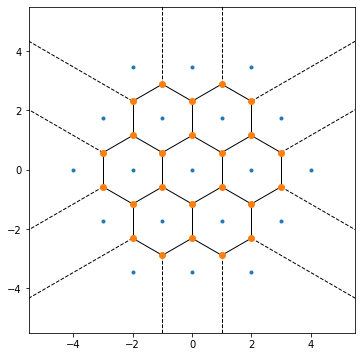
\includegraphics[width=0.5\textwidth]{voronoi.png}
    \caption{Voronoi tesselation of initial cell placement. Cell bodies shown in blue points, collar boundaries shown in black lines with collar boundary end points shown in orange. Notably, the regions corresponding to boundary cells extend out to infinity. We need to add all boundary collar vertices along the infinite dashed lines.}
    \label{fig:voronoi}
\end{figure}

\subsubsection{Boundary collar vertices} \label{subsubsec:bdary_verts}

We ask whether boundary collar vertices contribute to the energy. For boundary cells $\alpha, \beta$, suppose the line of physical interactions between the two cells' microvilli spans from point $\bm{r}_\rho$  and ends at point $\bm{r}_\sigma$. We with to know how the angle between the planes given by points $\rho, \alpha, \sigma$ and $\rho, \beta, \sigma$ changes with the position of boundary collar vertex $\sigma$. 

Suppose for the time being that the collar length is fixed at $\ell$, so the possible values for $\bm{r}_\sigma$ are constrained. We simplify the problem by reparameterising our coordinates such that $\bm{r}_\alpha = (-1, 0, 0)$, $\bm{r}_\rho = (0, r, 0)$, and $\bm{r}_\beta = (1, 0, 0)$, where $r = \sqrt{\ell^2 - 1}$. Here, $\ell$ is a dimensionless ratio of the collar length to half the cell-cell distance. We readily see that $\bm{r}_\sigma = (x, y, z)$ is constrained to take values in the circle defined by $r^2 = y^2 + z^2, x=0$. 

Parameterising the positions of $\bm{r}_\sigma(\theta) = (0, r\cos\theta, r\sin\theta)$ by angle $\theta$ with the second axis, we find the normals for planes $\rho, \alpha, \sigma$ and $\rho, \beta, \sigma$ as 

\begin{align*}
	\bh{n}_{\rho\alpha\sigma} &= (\bm{r}_\sigma - \bm{r}_\alpha) \times (\bm{r}_\rho - \bm{r}_\alpha) \\
	&= \frac{(-r^2 \sin\theta, r\sin\theta, r - r\cos\theta)}{r^4\sin^2\theta + 2r^2(1-\cos\theta)} \\
	\bh{n}_{\rho\beta\sigma} &= (\bm{r}_{\rho} - \bm{r}_\beta) \times (\bm{r}_\sigma - \bm{r}_\beta)\\
	&= \frac{(r^2 \sin\theta, r\sin\theta, r\cos\theta - r)}{r^4\sin^2\theta + 2r^2(1-\cos\theta)}.
\end{align*}

\noindent After simplifying, the angle between these two normal vectors is 

\begin{align}
	\bh{n}_{\rho\alpha\sigma} \cdot \bh{n}_{\rho\beta\sigma} &= 1 - \frac{2}{1 + \frac{1}{2r^2} \left( 1 + \tan^2 \frac{\theta}{2}\right)}. \label{eq:changing_angle}
\end{align}

It is clear that the position of the boundary collar interaction at $\bm{r}_\sigma$ changes the angle between these two planes, given by the arccosine of \cref{eq:changing_angle}. In the simplified sheet structure defined in the combined cell-collar graph $\mathfrak{G}$, this results in a change in energy based on the position of $\bm{r}_\sigma$. Consequently, as the notation indicates, boundary collar vertices are introduced to $\mathfrak{G}$ connecting between each pair of boundary cells.

\subsubsection{Adding boundary collar vertices}

Defining initial positions for boundary collar vertices becomes challenging when sheets are not planar, though a reasonable placement is sufficient since the positions will be changed later. For sheets in the $xy$-plane generated by 2-dimensional Voronoi tesselation (\cref{fig:voronoi}), ridges extending out to infinity are removed and replaced with collar vertices at finite distance. The position of a boundary collar vertex $\sigma$ between cells $\alpha, \beta$ is calculated as follows. 
First, a unit vector $\bh{n}$ perpendicular to the ridge between cell positions $\bm{r}_\alpha, \bm{r}_\beta$ is determined. 
For sheets in the $xy$-plane, $\bh{n}=\hat{z}$. Otherwise, $\bh{n}$ is simply aligned with the average of the normal vectors $\bh{n}_\alpha, \bh{n}_\beta$.
Then, the boundary collar vertex position $\bm{r}_\sigma$ is positioned at the reflection of $\bm{r}_\rho$ over the plane given by points $\bm{r}_\alpha, \bm{r}_\beta, \bm{r}_\alpha + \bh{n}$, where $\rho$ is the existing collar vertex shared by $\alpha$ and $\beta$.
Notably, this process results in a boundary collar position $\bm{r}_\sigma$ farther from the center of the sheet than $\bm{r}_\rho$ and equidistant to $\bm{r}_\alpha, \bm{r}_\beta$ as $\bm{r}_\rho$. 

This process produced reasonable boundary collar vertex positions to initialise sheet dynamics simulations (\cref{fig:layout_init}). For initial collar positions not too far from cells, collars did not overlap or cross over each other. Some initial graphs $\mathfrak{G}$ are shown projected onto the $xy$-plane, though the collars are offset in $z$ (\cref{subfig:layout_init_planar}) or the entire sheet is not necessarily lying in the $xy$-plane (\cref{subfig:layout_init_curved}).

\mynote{add to figure \ref{fig:layout_init}}

\begin{figure}[hbtp]
    \centering
    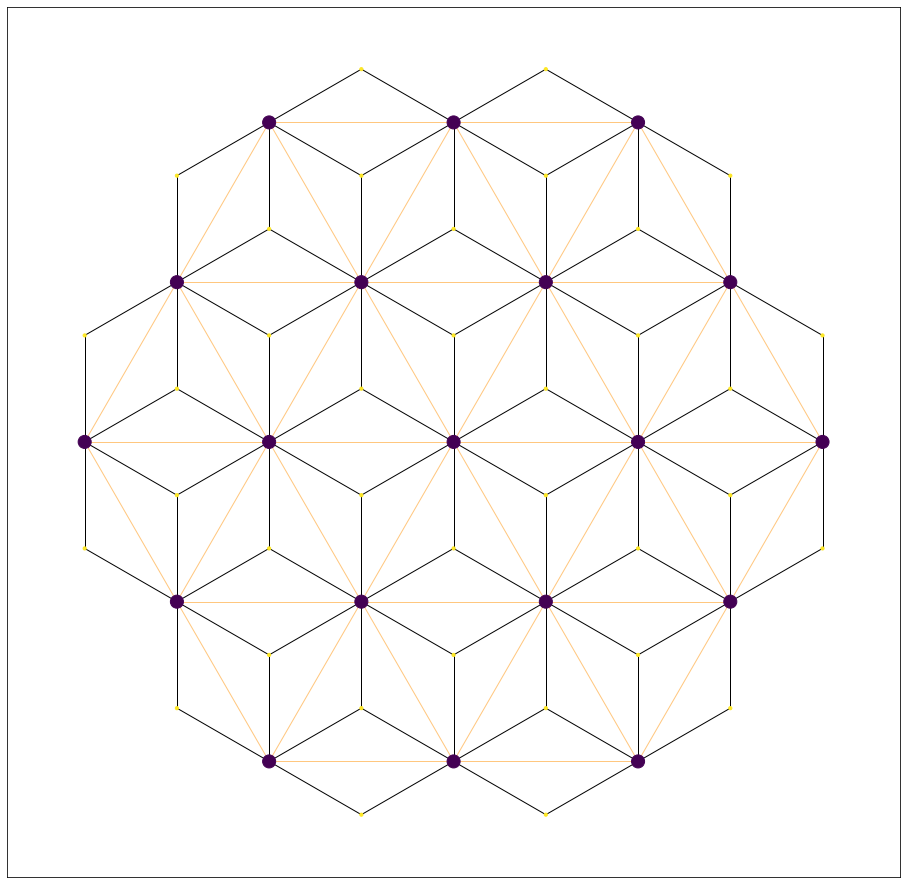
\includegraphics[width=0.8\textwidth]{layout_init.png}
    \caption{Initial layout for the flexa sheet. Cell bodies are shown in large purple points and collar boundary vertices are shown in small yellow points. Black edges connect cells to collar boundary vertices, and orange edges show cell-cell neighbor relations (though these orange edges are not physically present). The physical interactions are mediated through the black edges.}
    \label{fig:layout_init}
\end{figure}

\section{Sheet energy}

In developing the simplified, discrete model for \textit{C. flexa} as a spatial graph, I aim to distill the complex physics of collar-collar interactions into a minimum number of sufficient energy terms to capture the sheet bending that we observe experimentally. In what follows, I treat edges $(\alpha, \rho)$ between a cell $\alpha$ and collar vertex $\rho$ as straight line collar microvilli and cell pairs, flanking collar pairs $(\alpha, \beta: \rho, \sigma)$ as lines of interactions between the planes given by points $\rho, \alpha, \sigma$ and $\rho, \beta, \sigma$. 

Consequently, as detailed in the continuous model description of \cref{ch:2}, I build an energy function $\e$ that penalises deviations for angles $\phi$ and $\psi$, which describe angles between ($\phi$) collar microvilli and cell normal vectors $\bh{n}_\alpha$ and ($\psi$) plane normals $\bh{n}_{\rho\alpha\sigma}, \bh{n}_{\rho\beta\sigma}$.

\subsection{Cell-collar angle energy}
\subsubsection{Cell normal definition}
For a physical \textit{C. flexa} cell $\alpha$ with fixed position $\bm{r}_\alpha$ and fixed collar positions $\{\bm{r}_\rho\}_{\rho\in\alpha}$, we realise that the cell still has freedom in its rotation which we expect will contribute substantially to its energy. 
In other words, there should be an optimal rotation for the cell to minimise its mechanical energy. 
Since we treat \textit{C. flexa} cells as rotationally symmetric above the apicobasal axis, it suffices in our description to assign to each cell $\alpha$ in the graph $\mathfrak{G}$ a unit vector $\bh{n}_\alpha$ 

For simplicity, each vector $\bh{n}_\alpha$ is initially defined as the unit vector in the direction of $\sum_{\rho\in\alpha} \vec{\alpha\rho}$, where $\vec{\alpha\rho} = \bm{r}_\rho - \bm{r}_\alpha$.

\subsubsection{Energy $\e_\phi$}

Defining an energy term on the angle $\phi$ between a cell $\alpha$'s collars and the apicobasal axis $\bh{n}_\alpha$ is established on descriptions of \textit{Choanoeca} in the literature. 
\citet{brunet2019} describes the change in this angle as the result of exposure to light in \textit{C. flexa}.
Similarly, \citet{ellis1930} characterises the variation in $\phi$ observed in individual cells of \textit{C. perplexa}.

Consequently, we consider an energy term $\e_\phi(\{\bm{r}_\alpha, \bh{n}_\alpha\}, \{\bm{r}_\rho\})$ which penalises devation from a common equilibrium basal collar angle $\phi_0$:

\begin{align}
	\e_\phi(\{\bm{r}_\alpha, \bh{n}_\alpha\}, \{\bm{r}_\rho\}) &= \sum_{(\alpha, \rho)} \left(\phi_{(\alpha, \rho)} - \phi_0 \right)^2. \label{eq:e_phi}
\end{align}

The sum indicates summation over all cell-collar pairs $(\alpha, \rho)$ in the sheet $\mathfrak{G}$. The angle $\phi_{(\alpha, \rho)}$ is calculated entirely based on the cell normal vector $\bh{n}_\alpha$ and unit vector $\hat{\alpha\rho}$ pointing in the direction of $\bh{r}_\rho - \bh{r}_\alpha$:

\mynote{make this equation numbered and number other substantial equations}

\begin{align*}
	\phi_{(\alpha, \rho)} &= \arccos \left(\bh{n}_\alpha \cdot \hat{\alpha\rho} \right) = \arccos \left(\bh{n}_\alpha \cdot \frac{\hat{\alpha\rho}}{\left| \hat{\alpha\rho}\right|} \right).
\end{align*}

\subsubsection{Optimal cell normal vectors}

No other energy terms will depend on the cell normal vectors $\{ \bh{n}_\alpha \}$, so we ask now what the optimal normal vector for a cell is. Suppose a cell is at position $\bm{r}_\alpha$ with collar vertices at $\bm{r}_\rho$ for $\rho \in \alpha$. We can determine how the cell orients in order to minimise the collar energy with respect to $\bh{n}_\alpha$. 

For fixed $\alpha$, the cell orientation vector $\bh{n}_\alpha$ is constrained to have unit length. Hence, we solve the constrained optimisation of $\e_\phi$ by solving the Lagrange multiplier problem with multiplier $\lambda$

\begin{align}
    0 &= \frac{\partial \left[ \e_\phi \lambda\left( \left| \bh{n}_\alpha\right|^2 - 1\right) \right] }{\partial \bh{n}_\alpha} \label{eq:phi_lagrange1} \\
    0 &= \frac{\partial \left[ \e_\phi + \lambda\left( \left| \hat{\bm{n}}_\alpha\right|^2 - 1\right)\right] }{\partial \lambda}. \label{eq:phi_lagrange2}
\end{align}

Using the constraint (solution to \cref{eq:phi_lagrange2}) $| \bh{n}_\alpha |^2 = 1$, we solve 

\begin{align*} 
    \lambda \bh{n}_\alpha &= 2 \sum_{\rho\in\alpha} \left[ \arccos\left(\hat{\alpha\rho} \cdot \bh{n}_\alpha \right) - \phi_0 \right] \frac{-1}{\sqrt{1 - \left(\hat{\alpha\rho} \cdot \bh{n}_\alpha \right)^2 }} \hat{\alpha\rho} \\
    \lambda &= 2 \left| \sum_{\rho\in\alpha} \left[ \arccos\left(\hat{\alpha\rho} \cdot \hat{n}_\alpha \right) - \phi_0 \right] \frac{1}{\sqrt{1 - \left(\hat{\alpha\rho} \cdot \hat{n}_\alpha \right)^2 }} \hat{\alpha\rho} \right|.  
\end{align*}

\noindent Then the optimal normal vector solves the transcendental equation 

\begin{align}
    \bh{n}_\alpha &= \frac{\sum_{\rho\in\alpha} \left[ \arccos\left(\hat{\alpha\rho} \cdot \bh{n}_\alpha \right) - \phi_0 \right] \frac{-1}{\sqrt{1 - \left(\hat{\alpha\rho} \cdot \bh{n}_\alpha \right)^2 }} \hat{\alpha\rho} }{\sum_{\rho\in\alpha} \left[ \arccos\left(\hat{\alpha\rho} \cdot \bh{n}_\alpha \right) - \phi_0 \right] \frac{1}{\sqrt{1 - \left(\hat{\alpha\rho} \cdot \bh{n}_\alpha \right)^2 }} \hat{\alpha\rho}} \label{eq:optimal_n}
\end{align}

Clearly the cell normal vectors must be computed numerically whenever a cell is interacting with several other cells simultaneously in complicated geometries. 
We can choose to either approximate the normal vectors with a physically reasonable approximation or treat the normal vectors as free arguments to the energy function to be optimised.
I discuss both options below. 

\subsubsection{Approximating cell normal vectors}

There are several options for approximating a cell normal vector $\bh{n}_\alpha$ based on positions $\bm{r}_\alpha$ and $\{ \bm{r}_\rho\}_{\rho\in\alpha}$. The simplest option we might be able to think of is to let $\bh{n}_\alpha$ be the unit vector in the direction $\sum_{\rho\in\alpha}\hat{\alpha\rho}$. 
This approach has the benefit that collar vertices farther from $\bm{r}_\alpha$ are weighted more in the cell normal vector, agreeing with the intuition that a more distant collar interaction demands more cell rotation to accommodate it. 
However, we find that this approach results in unreasonable cell normal vectors for boundary cells as defined in $\mathfrak{G}$ since boundary cells do not have a full ring of boundary collar vertices. 
For this approach to work, $\mathfrak{G}$ would need to include several more collar vertices which do not describe interactions between cells and add unnecessary complexity.
In application, I found that the boundary cell effect of this choice of $\bh{n}_\alpha(\bm{r}_\alpha, \{\bm{r}_\rho\}_{\rho\in\alpha})$ substantially affected boundary collar vertex positions after energy equilibration and the overall energy landscape as a function of equilibrium angles $\phi_0, \psi_0$. 

When initialising a flat sheet, the above averaging approach also does not agree with intuition, since it results in boundary cell normal vectors that do not point in the same direction as normal vectors for cells not on the sheet boundary (\cref{fig:layout_init}). Instead, when a sheet lies flat in the $xy$-plane, it is expected that all vectors $\bh{n}_\alpha$ point in the $+\hat{z}$ direction provided that collars are above cells in $\bm{z}$. 
A viable alternative is to define $\bh{n}_\alpha$ by taking a plane approximation to cell $\alpha$'s collar vertices. 
The normal vector to this plane oriented away from the cell defines a normal vector that agrees with intution and supports calculating normals for a non-coplanar set of collar vertices.

The plane approximation approach is easiest achieved using ordinary least squares. 
Briefly, we approximate $\hat{r}_{\rho 3} = (r_{\rho 1}, r_{\rho 2}) \cdot (\beta_1, \beta_2) + \beta_0$ and minimise the sum of squared residuals $\sum_{\rho\in\alpha} (\hat{r}_{\rho 3} - r_{\rho 3})^2$ with respect to $\beta_0, \beta_1, \beta_2$. 
The normal vector of the plane approximation is then $(\beta_1, \beta_2, -1)$ up to normalisation and multiplication by $-1$.\footnote{The notation here is chosen to be consistent with that typically used in ordinary least squares, hence the hatted values indicate an approximation rather than vector normalisation as I use otherwise.} 

\subsection{Cell-cell junction angle $\psi$ energy} \label{subsec:e_psi}

As in \cref{ch:2}, we aim to produce sheet curvature with the angle $\psi$ that two cells' collars make at their interface. As in \cref{subsubsec:bdary_verts}, we calculate the angle between planes defined by two cells $\alpha, \beta$ and their mutual flanking collar vertices $\rho, \sigma$ with

\begin{align}
	\psi_{(\alpha, \beta: \rho, \sigma)} &= \frac{\pi}{2} - \frac{1}{2}\arccos \left(\bh{n}_{\rho\alpha\sigma} \cdot \bh{n}_{\rho\beta\sigma} \right) \label{eq:psi}
\end{align}

The normal vectors $\bh{n}_{\rho\alpha\sigma}$ for a plane given by points $\rho, \alpha, \sigma$ must have a systematically defined orientation, as they can point in either direction $\pm (\bm{r}_\rho - \bm{r}_\alpha) \times (\bm{r}_\sigma - \bm{r}_\alpha)$. 
In the geometry used to define $\psi$ in \cref{eq:psi}, the collar-cell-collar normal vectors are assumed to be pointing in the direction of the cells' flagella. 
With the simplifying assumption that the cell normal always points in the inside of the collar, we have that the collar-cell-collar normals must take orientation to align with their corresponding cell normals. 
Consequently, we let $\bh{n}_{\rho\alpha\sigma}' = \vec{\alpha\rho} \times \vec{\alpha\sigma}$ and set $\bh{n}_{\rho\alpha\sigma} = \sgn (\bh{n}_{\rho\alpha\sigma}' \cdot \bh{n}_\alpha) \bh{n}_{\rho\alpha\sigma}'$.\footnote{Here $\sgn$ is the sign operator.}

Defining $\bh{n}_{\rho\alpha\sigma}$ in this way makes it dependent on the cell normal vectors $\bh{n}_\alpha$. 
However, when minimising the energy, I work to develop methods such that $\sgn (\bh{n}_{\rho\alpha\sigma} \cdot \bh{n}_\alpha)$ remains constant. 
This corresponds to ensuring that no collar vertices cross through each other (corresponding to microvilli crossing over each other) and that the cell normal vectors remain pointing inside the collars.
Hence, I effectively treat the effect of $\bh{n}_\alpha$ on a collar-cell-collar normal vector $\bh{n}_{\rho\alpha\sigma}$ to be constant.

With a common equilibrium collar-collar interface angle $\psi_0$ (as all cells are assumed equal in their mechanical properties), we express the energy $\e_\psi$ 

\begin{align}
	\e_\psi &= k_\psi \sum_{(\alpha, \beta: \rho, \sigma)} (\psi_{(\alpha, \beta: \rho, \sigma)} - \psi_0)^2. \label{eq:e_psi}
\end{align}

\subsection{Collar length}

To provide sufficient flexibility to sheets through collar microvilli, I introduce an energy term $\e_{\text{sp}}$ defined by 

\begin{align}
	\e_{\text{sp}} &= k_{\text{sp}} \sum_{(\alpha, \rho)} \left| \vec{\alpha\rho} - \ell_{0\alpha\rho} \right|^2, \label{eq:e_sp}
\end{align}

\noindent where $\ell_{0\alpha\rho}$ is an equilibrium length for edge $(\alpha, \rho)$. The sum indicates summation over all cell, collar pairs $(\alpha, \rho)$ in the sheet $\mathfrak{G}$.

All cells are assumed to take identical properties, so all values $\ell_{0\alpha\rho}$ are set to a constant $\ell_0$ unless indicated otherwise. When done so, we find that $\ell_0$ is the only length defined in the problem.

When interested in sheets with constrained collar length, we may either take a numerical approach or exploit the above energy term by setting $k_{\text{sp}}$ to a large value. The former is discussed in \cref{subsec:numerical}.


\section{Minimising sheet energy}

\mynote{resume from here}

We now have an energy $\e\{ \bm{r}_v \}_{v \in \mathfrak{G}} = \e_\phi + \e_\psi$ which is parameterised over the cell and collar boundary vertex positions. Notably, we treat the topology of the network as fixed, so the indices of the summations for $\e_\phi$ and $\e_\psi$ are unchanged even as we minimise energy.

\subsubsection{Flat sheet as a solution} \label{subsubsec:flat}

Notice that we have a pair $(\phi_0, \psi_0)$ that gives $\e = \e_\phi + \e_\psi = 0$. Since the $\phi$ and $\psi$ energies are nonnegative, the flat sheet is a stable minimum. 

\subsubsection{Constant collar length constraint}

For now, we are numerically constraining the cell-collar lengths at $\ell$, their initial lengths (which are constant for all cells). If we want to use the generalisability of our model to use an random initial cell distribution and generate the irregular boundaries with Voronoi tesselation, we will have to relax this condition and add a collar length spring energy to $\e$. The constant collar length constraint only applies to sheets generated by regular lattices when laid flat on a plane.


The constraint is defined by a vector function $f((c, b)) = |\bm{r}_c - \bm{r}_b| - \ell = 0$ for all cell-collar edges $(c, b)$. If $n_{\text{collars}}$ is the number of cell-collar edges in $\{\text{cell-collar edges }(c,b) \}$, then $f$ defines a $n_{\text{collars}}$-vector function. 

My optimisation routine requires that we calculate a Jacobian matrix for the vector constraint function. This gets ugly if we use $f$ as written above, but it is fortunately equivalent to set the constraint $f'((c, b)) = |\bm{r}_c - \bm{r}_b|^2 - \ell^2 = 0$. It is an interesting problem to take the gradient of $\bm{f'}$ with respect to all of the coordinates, but I won't include it here. It's implemented in my code.

\subsubsection{Solving sheet shape}

Numerical optimisation: sensitivity issues and initial conditions

Derive the gradient

Describe how to compute the gradient in an efficient way

\subsection{Graph topology}
For hexagonal lattice start, we 

Call back to section \ref{sec:c_1d}

\section{Energy gradient descent}

Due to the instability of the numerical optimisation routine used above, I moved to minimising the total energy $\e$ explicitly using gradient descent. 
The goal in taking this approach is to explicitly calculate the gradients $\partial \e / \partial \bm{r}_\gamma$ of the energy with respect to all coordinate vectors $\bm{r}_\gamma$ and incrementally take small steps in the reverse direction. 

Although gradient descent in several contexts is criticised for being slow and by nature prone to be trapped in local minima, in the context of modeling \textit{C. flexa} sheets it is preferable to a black box optimisation routine. Calculating the gradient analytically amounts to calculating the forces on all coordinates, and taking incremental steps in the direction of the negative gradient amounts to forward integrating Newton's laws $F_\gamma = - \partial\e/\partial\bm{r}_\gamma$. 
Consequently, we gain access to the dynamics induced by the simplified model that I describe above. 
Moreover, the susceptibility of this approach to be trapped in local minima is ideal not only from an energetic perspective, but also from a numerical one: by taking incremental steps in a direction known to decrease the energy, any increases indicate a flaw and \mynote{and what??}

In contrast to a numerical optimisation routine, gradient descent requires substantial explicit calculation. Moreover, the algorithm requires tuning in the step size and relative decrease in energy tolerance at which to decide the algorithm has terminated. 

\subsection{Deriving the gradient}

The linearity of the gradient permits us to take the gradient term-by-term in \cref{eq:energy_disc}. For an energy function $\e(\{ \bm{r}_\gamma\})$ with cell normal vectors $\bh{n}_\alpha$ approximated in terms of each cell's collar vertices, we find that the gradient $\partial \e_\phi / \partial \bm{r}_\gamma$ is given by 

\begin{align}
	phi eq \label{eq:grad_phi}
\end{align}

\mynote{describe how this can be simplified as a matrix mult problem}

As discussed in \ref{subsec:e_psi}, an angle $\psi_{(\alpha, \beta: \rho, \sigma)}$ for a cell-cell interface depends in a piecewise constant way on the cells' normal vectors. While the angles are consequentially only piecewise differentiable, gradient descent makes reasonable the assumption that there will not be any discontinuities in $\e_\psi$ for sufficiently small steps in the direction of the negative gradient. The below expression for $\partial \e_\psi / \partial \bm{r}_\gamma$ assumes that the sign of $\bh{n}_\alpha \cdot (\vec{\alpha\rho}\times \vec{\alpha\sigma})$ remains constant.

\begin{align}
	psi eq \label{eq:grad_psi}
\end{align}

The gradient $\partial \e_{\text{sp}} / \partial \bm{r}_\gamma$ is given by the linear spring force 

\begin{align}
	spring eq \label{eq:grad_sp}
\end{align}

\subsection{Forward integration}

Integrating the gradient given by equations \cref{eq:grad_phi,eq:grad_psi,eq:grad_sp} produces the dynamics of sheet bending as in \cref{fig:dynamics}. 
\mynote{discuss the equilibrium states}

\begin{align}
	\bm{r}_\gamma(t+\Delta t) &= \bm{r}_\gamma (t) - \Delta t \frac{\partial \e}{\partial \bm{r}_\gamma}. \label{eq:grad_desc_r}
\end{align}

When treating the normal vectors $\bh{n}_\alpha$ as free variables, we must solve modify our force equilibration algorithm to maintain the constraint that $| \bh{n}_\alpha |^2 = 1$. 
An intuitive option is to step in the direction of the negative gradient and normalise the intermediate vectors at each step:

\begin{align}
	\bm{n}_\alpha(t+\Delta t) &= \bh{n}_\alpha(t) - \Delta t \frac{\partial \e}{\partial \bh{n}_\alpha} \label{eq:grad_desc_n1}\\
	\bh{n}_\alpha(t+\Delta t) &= \frac{\bm{n}_\alpha(t+\Delta t)}{\bm{n}_\alpha(t+\Delta t)}. \label{eq:grad_desc_n2}
\end{align}

Equivalently, since for a sufficiently small step size the nearest point on the constraint set $|\bh{n}_\alpha|^2=1$ to $\bm{n}_\alpha(t+\Delta t)$ is unique, we may re-express \cref{eq:grad_desc_n2} with $\bh{n}_\alpha(t + \Delta t) = \arg \min_{|\bh{n}_\alpha|^2 = 1} |\bh{n}_\alpha - \bm{n}_\alpha(t+\Delta t)|$.
Expressed in this way, we see that the update for $\bh{n}_\alpha$ expressed in \cref{eq:grad_desc_n1,eq:grad_desc_n2} is exactly the projected gradient descent algorithm and we expect it to converge \citep{eicke1992}.
Since the normal component of $\partial \e / \partial \bh{n}_\alpha$ to the constraint set $|bh{n}_\alpha|^2 = 1$ at step $t$ does not affect $\bh{n}_\alpha(t + \Delta t)$, we can interpret \cref{eq:grad_desc_n1,eq:grad_desc_n2} as taking a step in the direction of the tangent space to the constraint set that reduces $\e$ the most.

\mynote{discuss the dynamics}

\begin{figure}
	\caption{todo}
	\label{fig:dynamics}
\end{figure}

While the forward integration works well for small sheets with simple graph topologies, I found that some equilbrium angles $\phi_0, \psi_0$ caused the sheet to strain to such an extreme that collar vertices would cross through each other. 
The resulting increase in energy comes from the discontinuous sign function in the definition of $\psi$ (\cref{eq:psi}), and collar vertices cross over each other due to too large of a step size $\Delta t$. 
While adaptively decreasing the step size is a viable option, it would substantially slow the equilibration algorithm.  
Instead, I introduced an additional term to the energy $\e_\varphi$ based on the angles $\varphi_{\rho\alpha\sigma}$ formed by each cell $\alpha$ and its adjacent pairs of collar vertices $\rho,\sigma$ when projected onto the plane defined by the cell normal $\bh{n}_\alpha$ (\cref{fig:varphi}):

\begin{align}
	\e_\varphi &= k_\varphi \sum_{(\alpha,\beta:\rho\sigma)} \left(\varphi_{\rho\alpha\sigma} - \varphi_{0\rho\alpha\sigma} \right)^2, \label{eq:e_varphi}
\end{align}

\noindent where $\varphi_{0\rho\alpha\sigma}$ is an equilibrium projected collar-cell-collar angle for each triple. 
Each angle $\varphi_{0\rho\alpha\sigma}$ is set to the actual value that is evaluated at the initial sheet geometry.
Unless specified otherwise, the constant $k_\varphi$ is set to $0.01k_\phi$.

\begin{figure}
	\centering 
	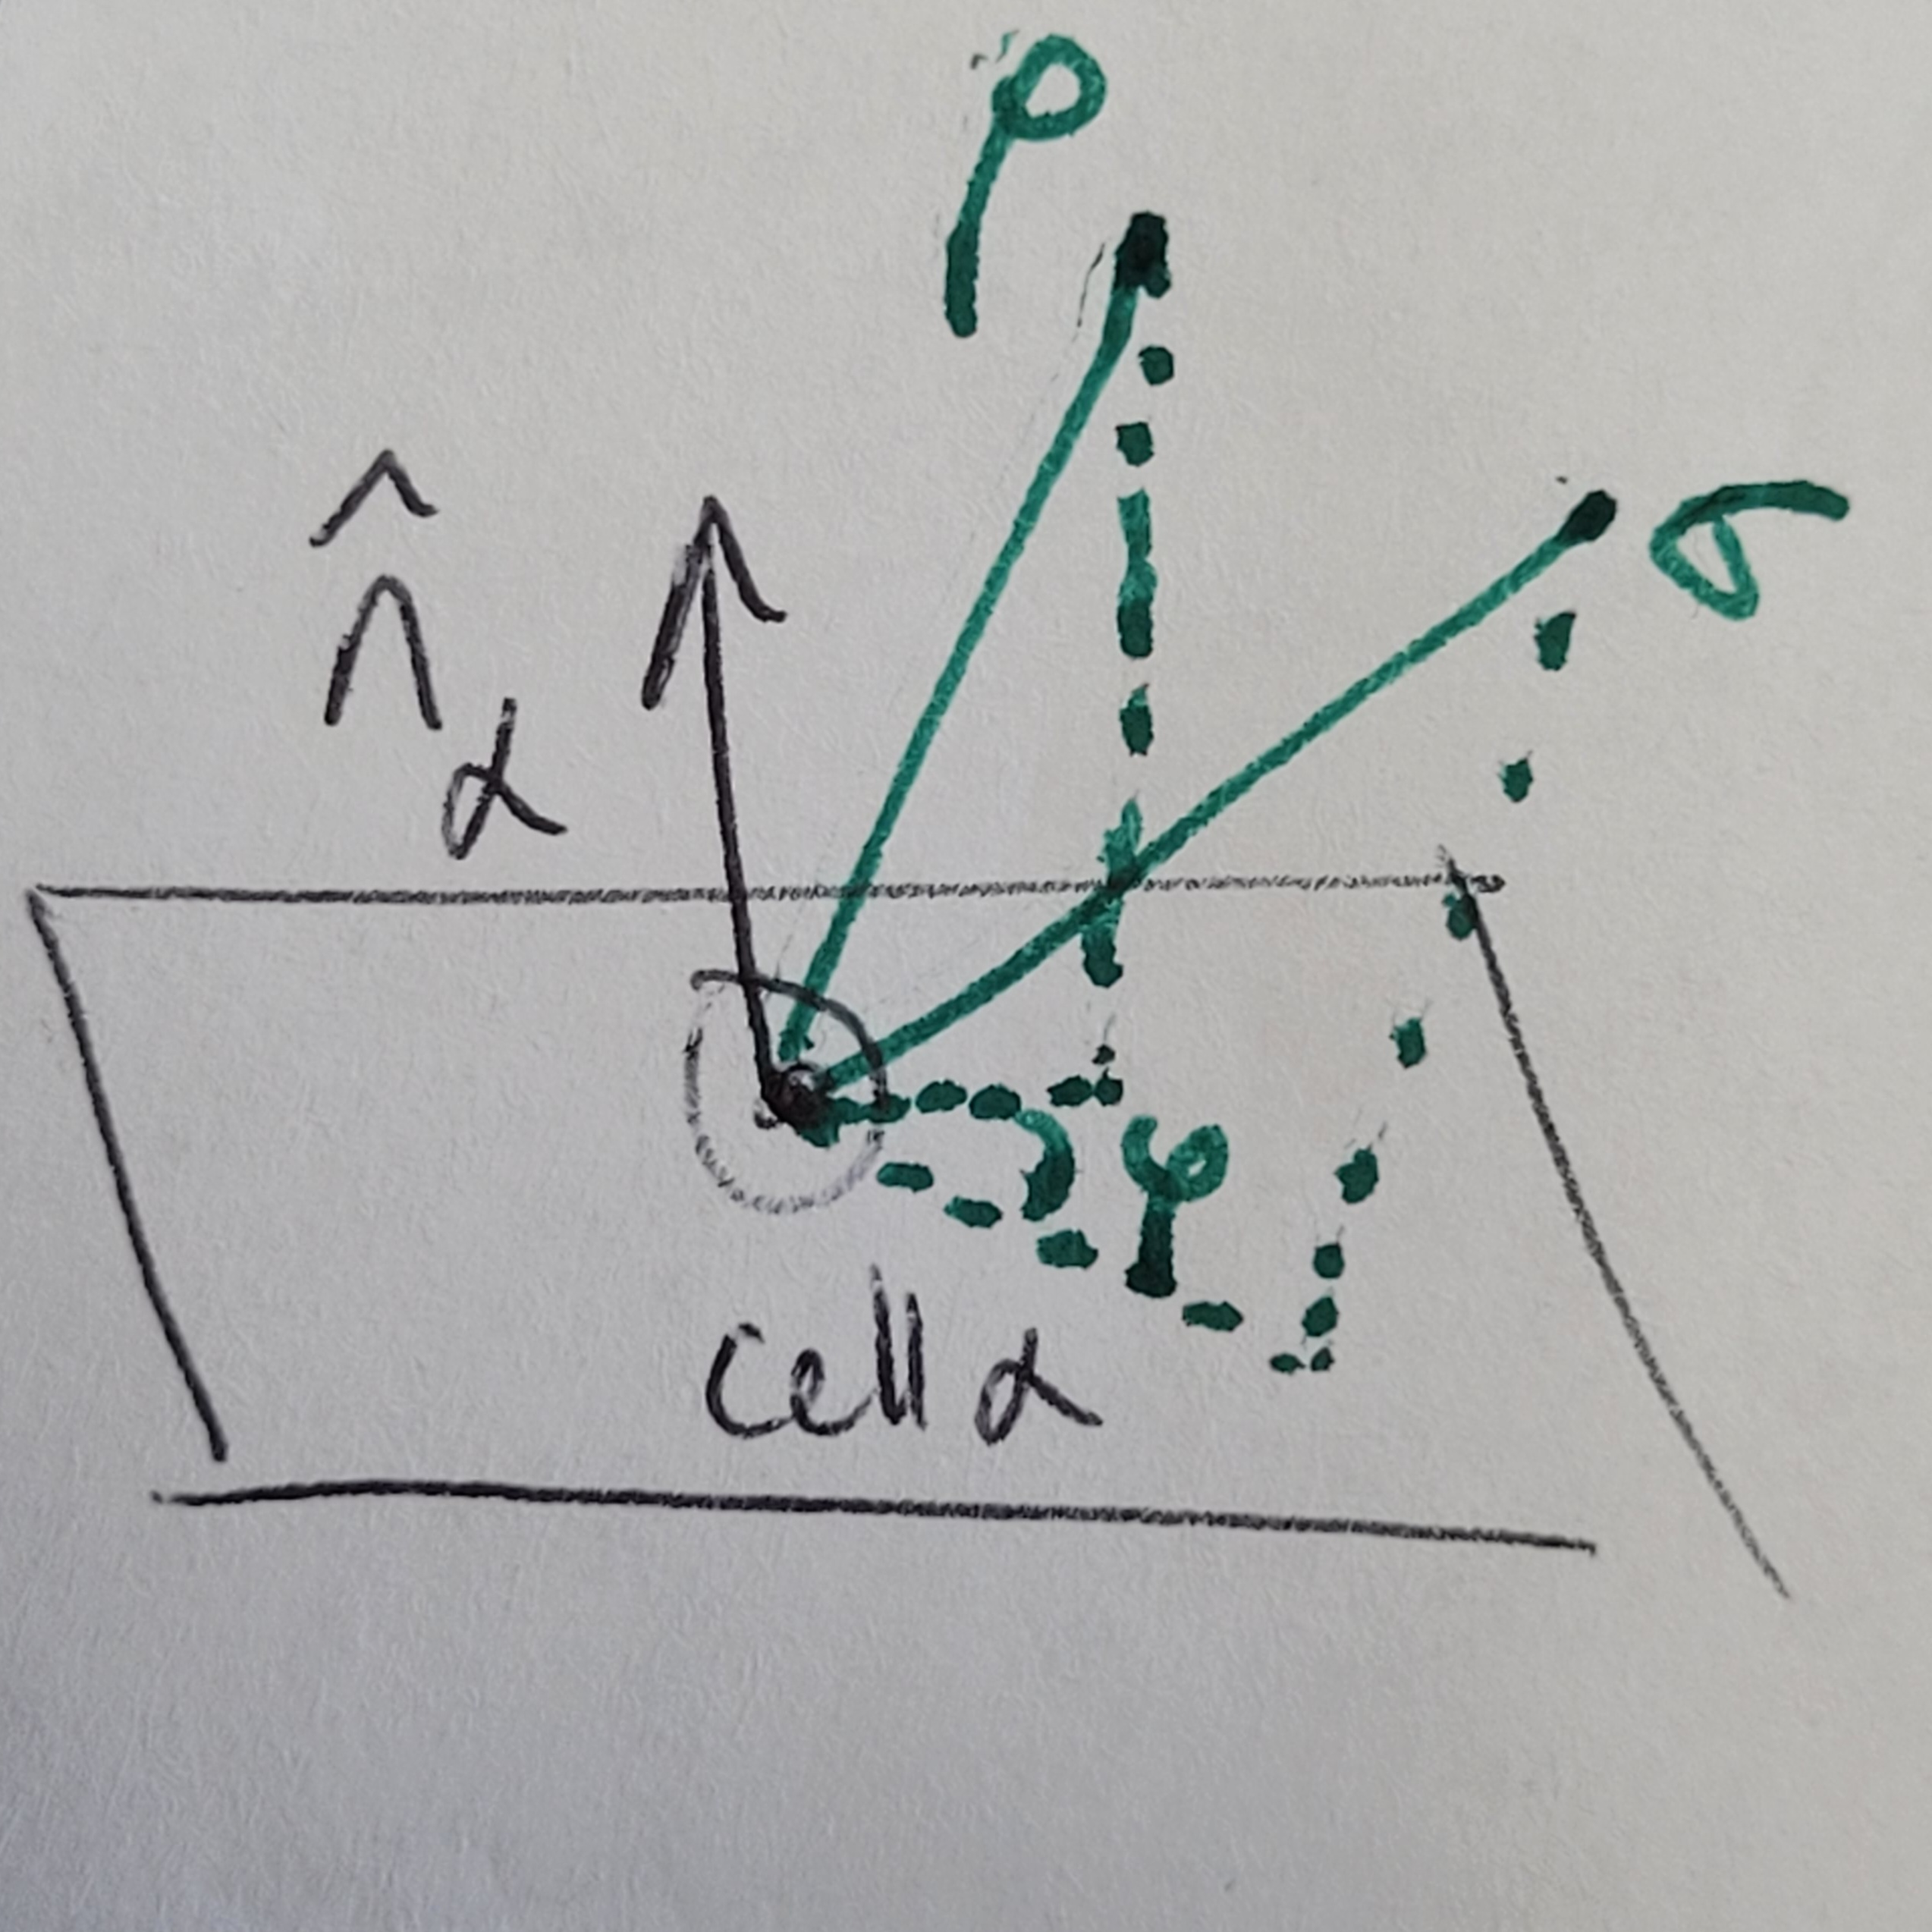
\includegraphics[width=0.5\textwidth]{varphi.jpg}
	\caption{Geometry for calculating $\varphi_{\rho\alpha\sigma}$.}
	\label{fig:varphi}
\end{figure}

The angles $\varphi_{\rho\alpha\sigma}$ are calculated similarly to $\phi, \psi$ (\cref{eq:phi,eq:psi},

\begin{align}
	\varphi_{\rho\alpha\sigma} &= \arccos \left[\vec{\alpha\rho}_\| \cdot \vec{\alpha\sigma}_\| \right], \label{eq:varphi}
\end{align}

\noindent where $\vec{\alpha\rho}_\|$ is the projection of $\vec{\alpha\rho}$ onto the plane defined by normal $\bh{n}_\alpha$ and position $\bm{r}_\alpha$. \mynote{give formula for $\vec{\alpha\rho}_\|$}
The gradient of $\e_\varphi$ is given by 

\begin{align}
	varphi eq \label{eq:grad_varphi}
\end{align}

\subsection{Exploring the energy landscape}

With the ability to study discrete sheet equilibrium geometries and dynamics, we are prepared to evaluate a mechanism for \textit{C. flexa} folding and inversion. 
Based on the two collar angle states observed in \citet{brunet2019}, a reasonable model would be to assume relaxed-state equilibrium angles $\phi_{\text{in}}, \psi_{\text{in}}$ and a different set of active-state angles $\phi_{\text{out}}, \psi_{\text{out}}$ with instantaneous transition between the two states. 
The rapid change in individual cell behavior and expected gradual sheet shape change expected from opposing cell-cell interactions align with our expectations from observations \citet{brunet2019}. 

Although we cannot access true values for the equilibrium angles, modeling \textit{C. flexa} sheets numerically provides the opportunity to explore the entire energy landscape. 
For sheets generated with a regular hexagonal lattice, we observe the expected diagonal valley where energy in minimised in the energy landscape since the sheet is expected to be flat along those pairs $(\phi_0, \psi_0)$ (\cref{fig:landscape_flat}).
Substantial sheet deformation and bending is evidently not sufficient to overcome the change in terms in the energy function. 
The increases in energy when the equilibrium angles are most disparate can be interpreted as collar microvilli stretching or compressing to accommodate sheet bending or a difference in the bending at each cell from the preferred state. 
For example, cells at neither the centre nor boundary in a bent sheet (\cref{fig:landscape_flat}, bottom-right or top-left) must contribute a positive contribution to $\e$ since they do not have the symmetric bending at all collar microvilli prescribed by \cref{eq:e_phi,eq:e_psi,eq:e_sp}.

\begin{figure}
	\centering
	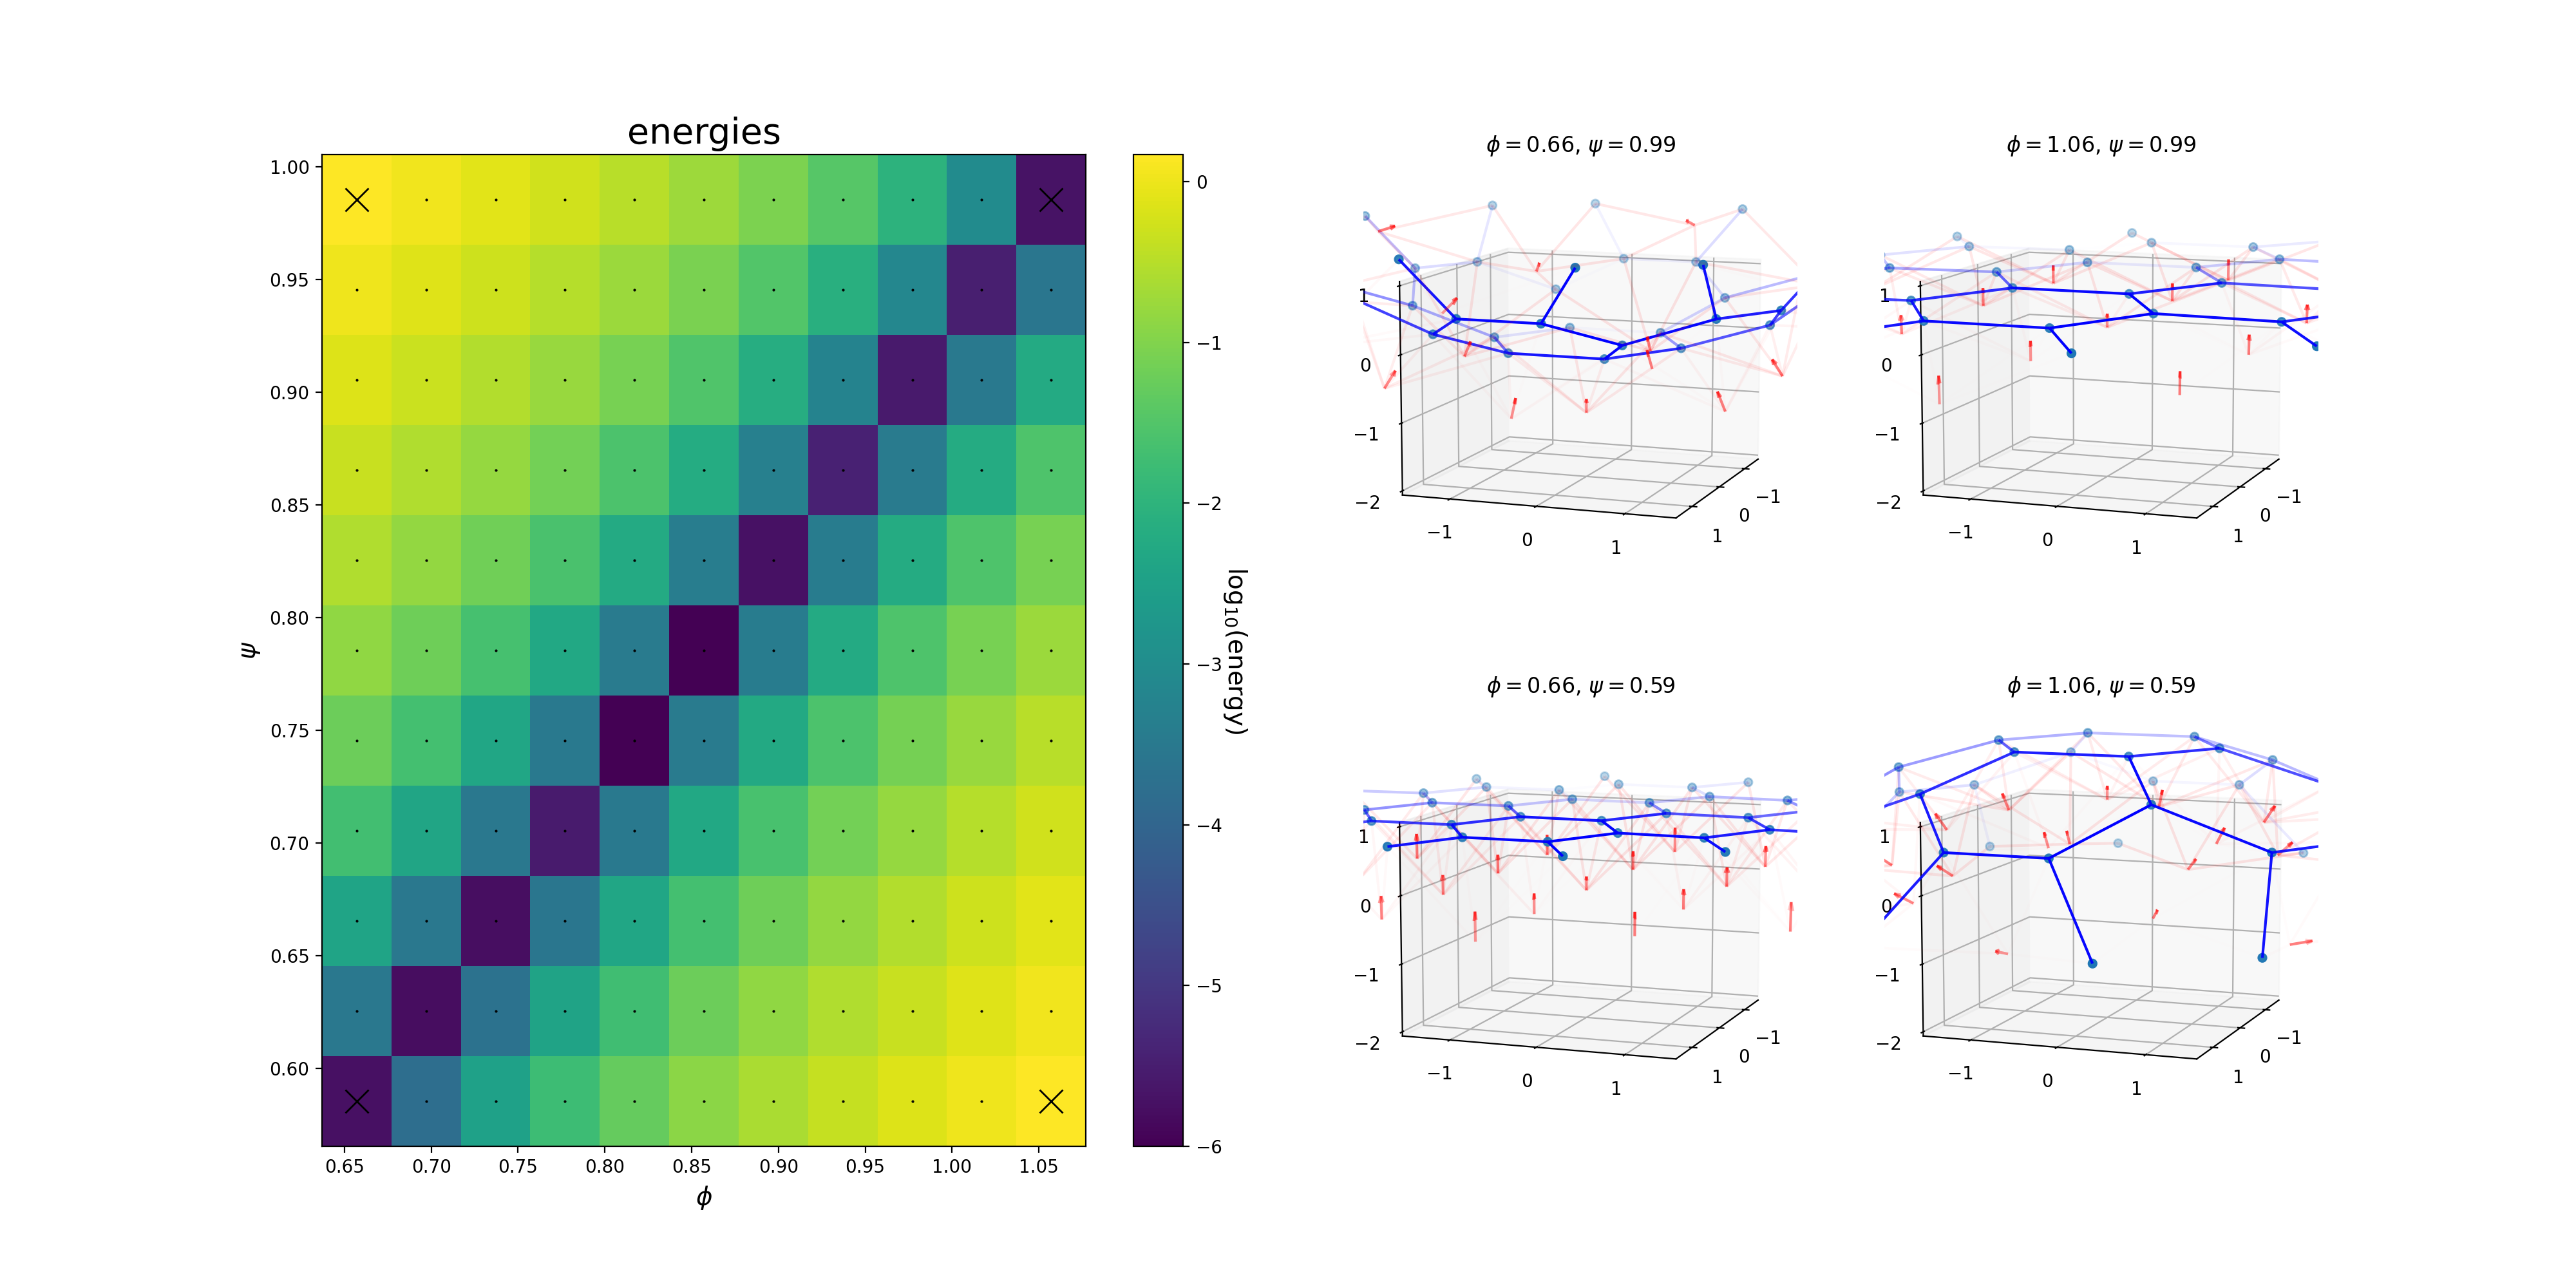
\includegraphics[width=\textwidth]{landscape_flat.png}
	\caption[Energy landscape of a discrete \textit{C. flexa} sheet generated from a hexagonal lattice]{Energy landcsape of a discrete \textit{C. flexa} sheet generated from a hexagonal lattice. Sheets displayed at the right correspond to the corners of the landscape indicated with white crosses.}
	\label{fig:landscape_flat}
\end{figure}

For graph topologies generated with an icosphere, we observe a more rich energy landscape (\cref{fig:landcsape_ico}).
Again we observe a similar minimum energy well running along a diagonal, though the energy increases at the ends since the network of cell-cell connections is not able to accommodate stretching and compression as readily as a sheet generated from a lattice.
Notably, the energy well for flagella-out sheets occurs in the region of high $\phi$ and low $\psi$. 
As predicted by \cref{eq:H0_phipsi}, $\phi > \psi$ results in a preferred curvature corresonding to a flagella-out sheet, in agreement with the observed energies.
Similarly, we see at these extremely disparate equilibrium angles that the edge of the flagella-in sheet begins to curve outward.
The fact that the equilibrium sheet demonstrates this stress indicates that inversion is constrained as a result of cell-cell connections and the collar stiffness $k_{\text{sp}}$.

For low $\psi$ and increasing $\phi$ in \cref{subfig:landscape_ico}, there appear to be sudden jumps in the energy profile. 
When investigated, it emerges that these jumps are the result of buckling at the sheet edges, where an increase in $\phi$ prompts boundary cells that wrap inward (\cref{subfig:landscape_ico}, bottom left) to push each other outward.
\mynote{get ico to invert for small sheets}

\begin{figure}
	\centering
	\begin{subfigure}[b]{\textwidth}
		\centering
		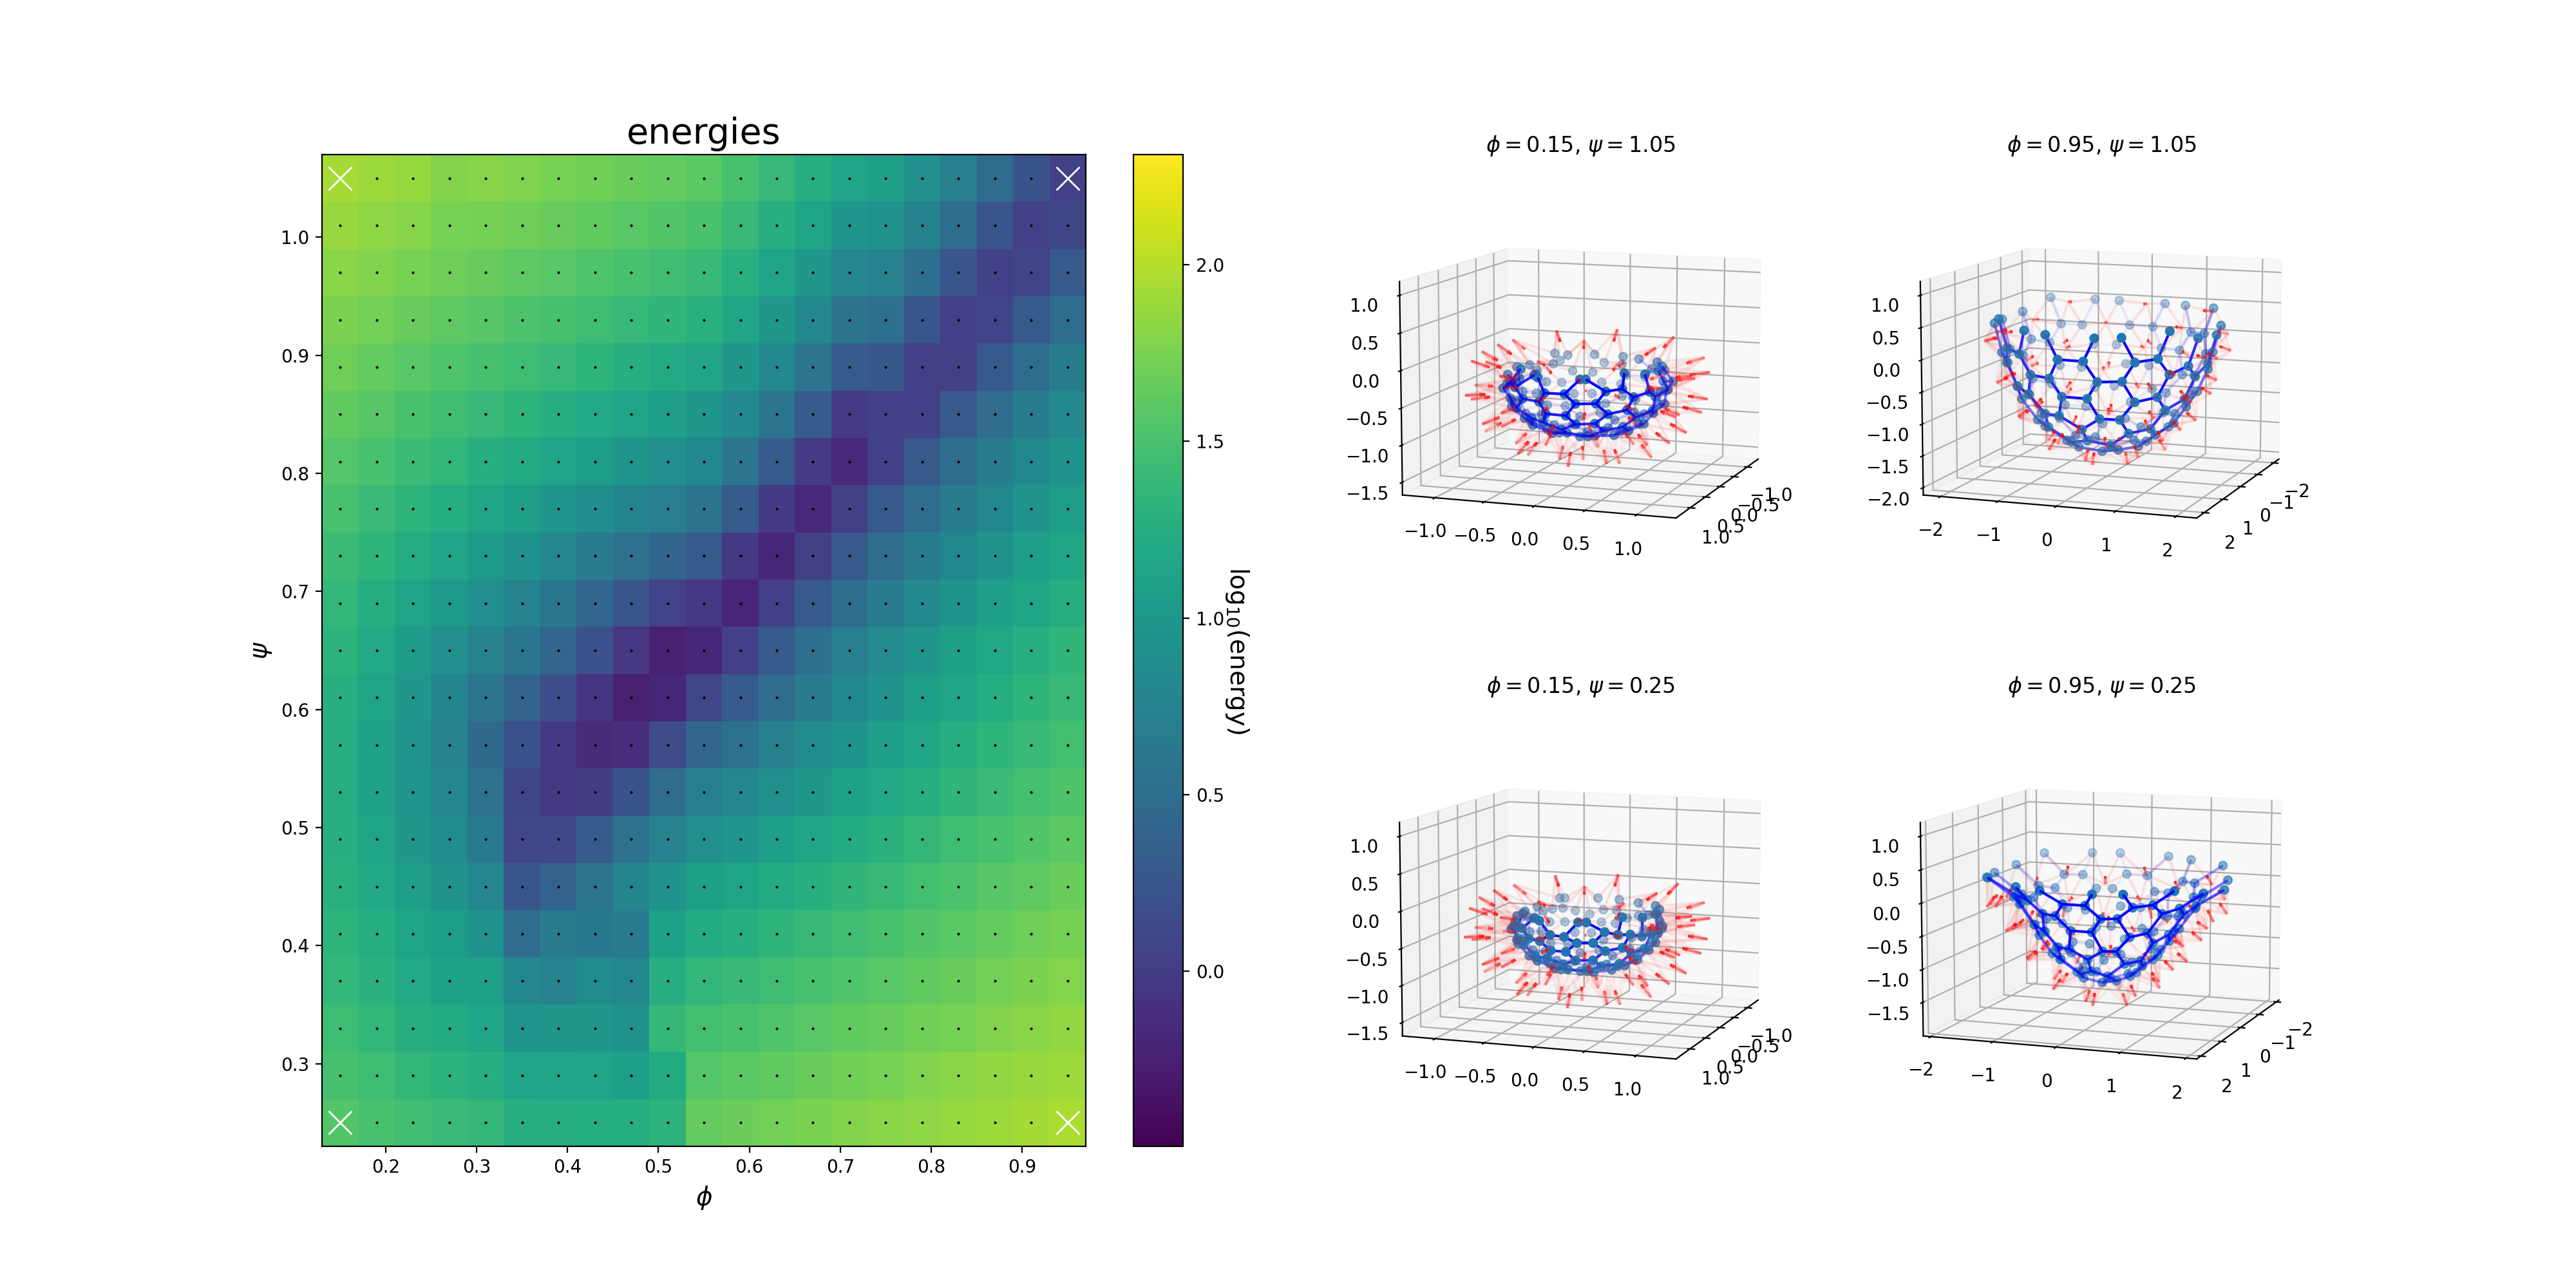
\includegraphics[width=\textwidth]{landscape_ico3.png}
		\caption{}
		\label{subfig:landscape_ico}
	\end{subfigure}
	\begin{subfigure}[b]{\textwidth}
		\centering
		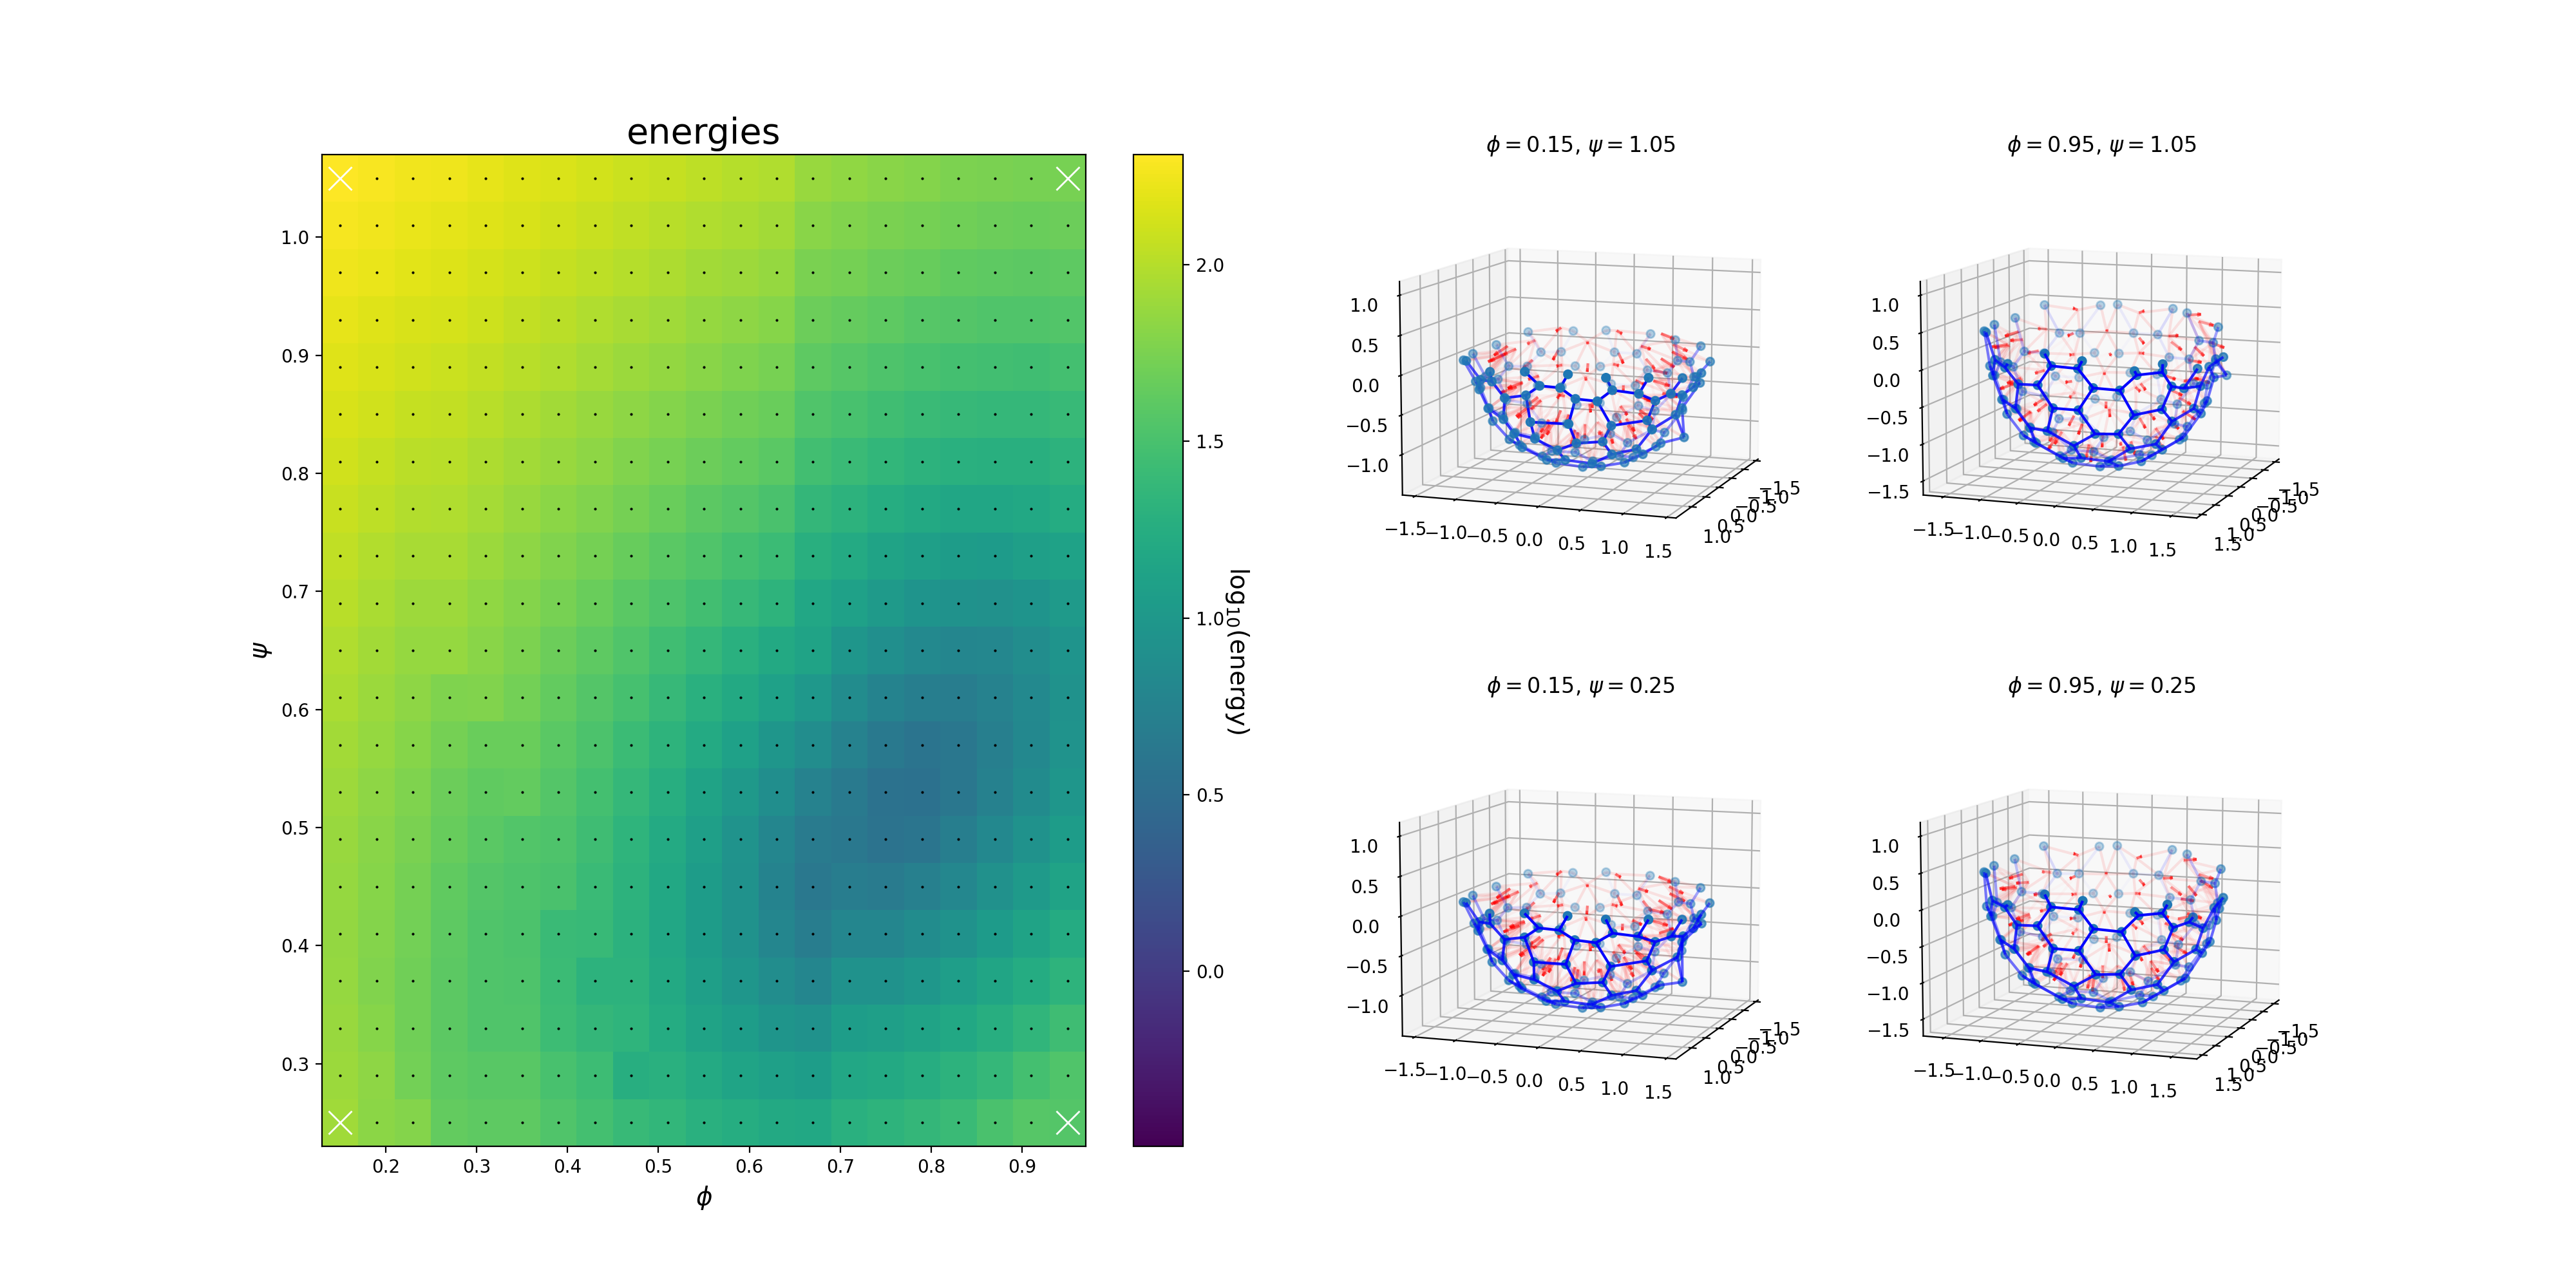
\includegraphics[width=\textwidth]{landscape_ico3r.png}
		\caption{}
		\label{subfig:landscape_icor}
	\end{subfigure}
	\caption[Energy landscape for flagella-in and flagella-out curved sheets]{Energy landscapes for (\ref{subfig:landscape_ico}) flagella-in and (\ref{subfig:landscape_icor}) flagella-out sheets of \textit{C. flexa}. The color scaling is the same in both images. The landscapes for a smaller segment of the icosphere were qualitatively similar.}
	\label{fig:landscape_ico}
\end{figure}

As we are interested in the bistability and transition in \textit{C. flexa} sheets, we are concerned with the global energy minima for both flagella-in and -out sheets. In \cref{fig:landscape_merge}, the minimum energy orientations throughout the landscape of \cref{fig:landscape_ico} are shown. 
As expected, the lowest possible energy can be achieved in the flagella-in orientation, consistent with the belief that cells are relaxed in this state \citep{brunet2019}.
With an increase in $\phi_0$ and decrease in $\psi_0$, corresponding to constriction in the apical myosin ring and flaring out or stiffening of the collar, the flagella-in state is preferred. 

\begin{figure}[ptbh]
	\centering
	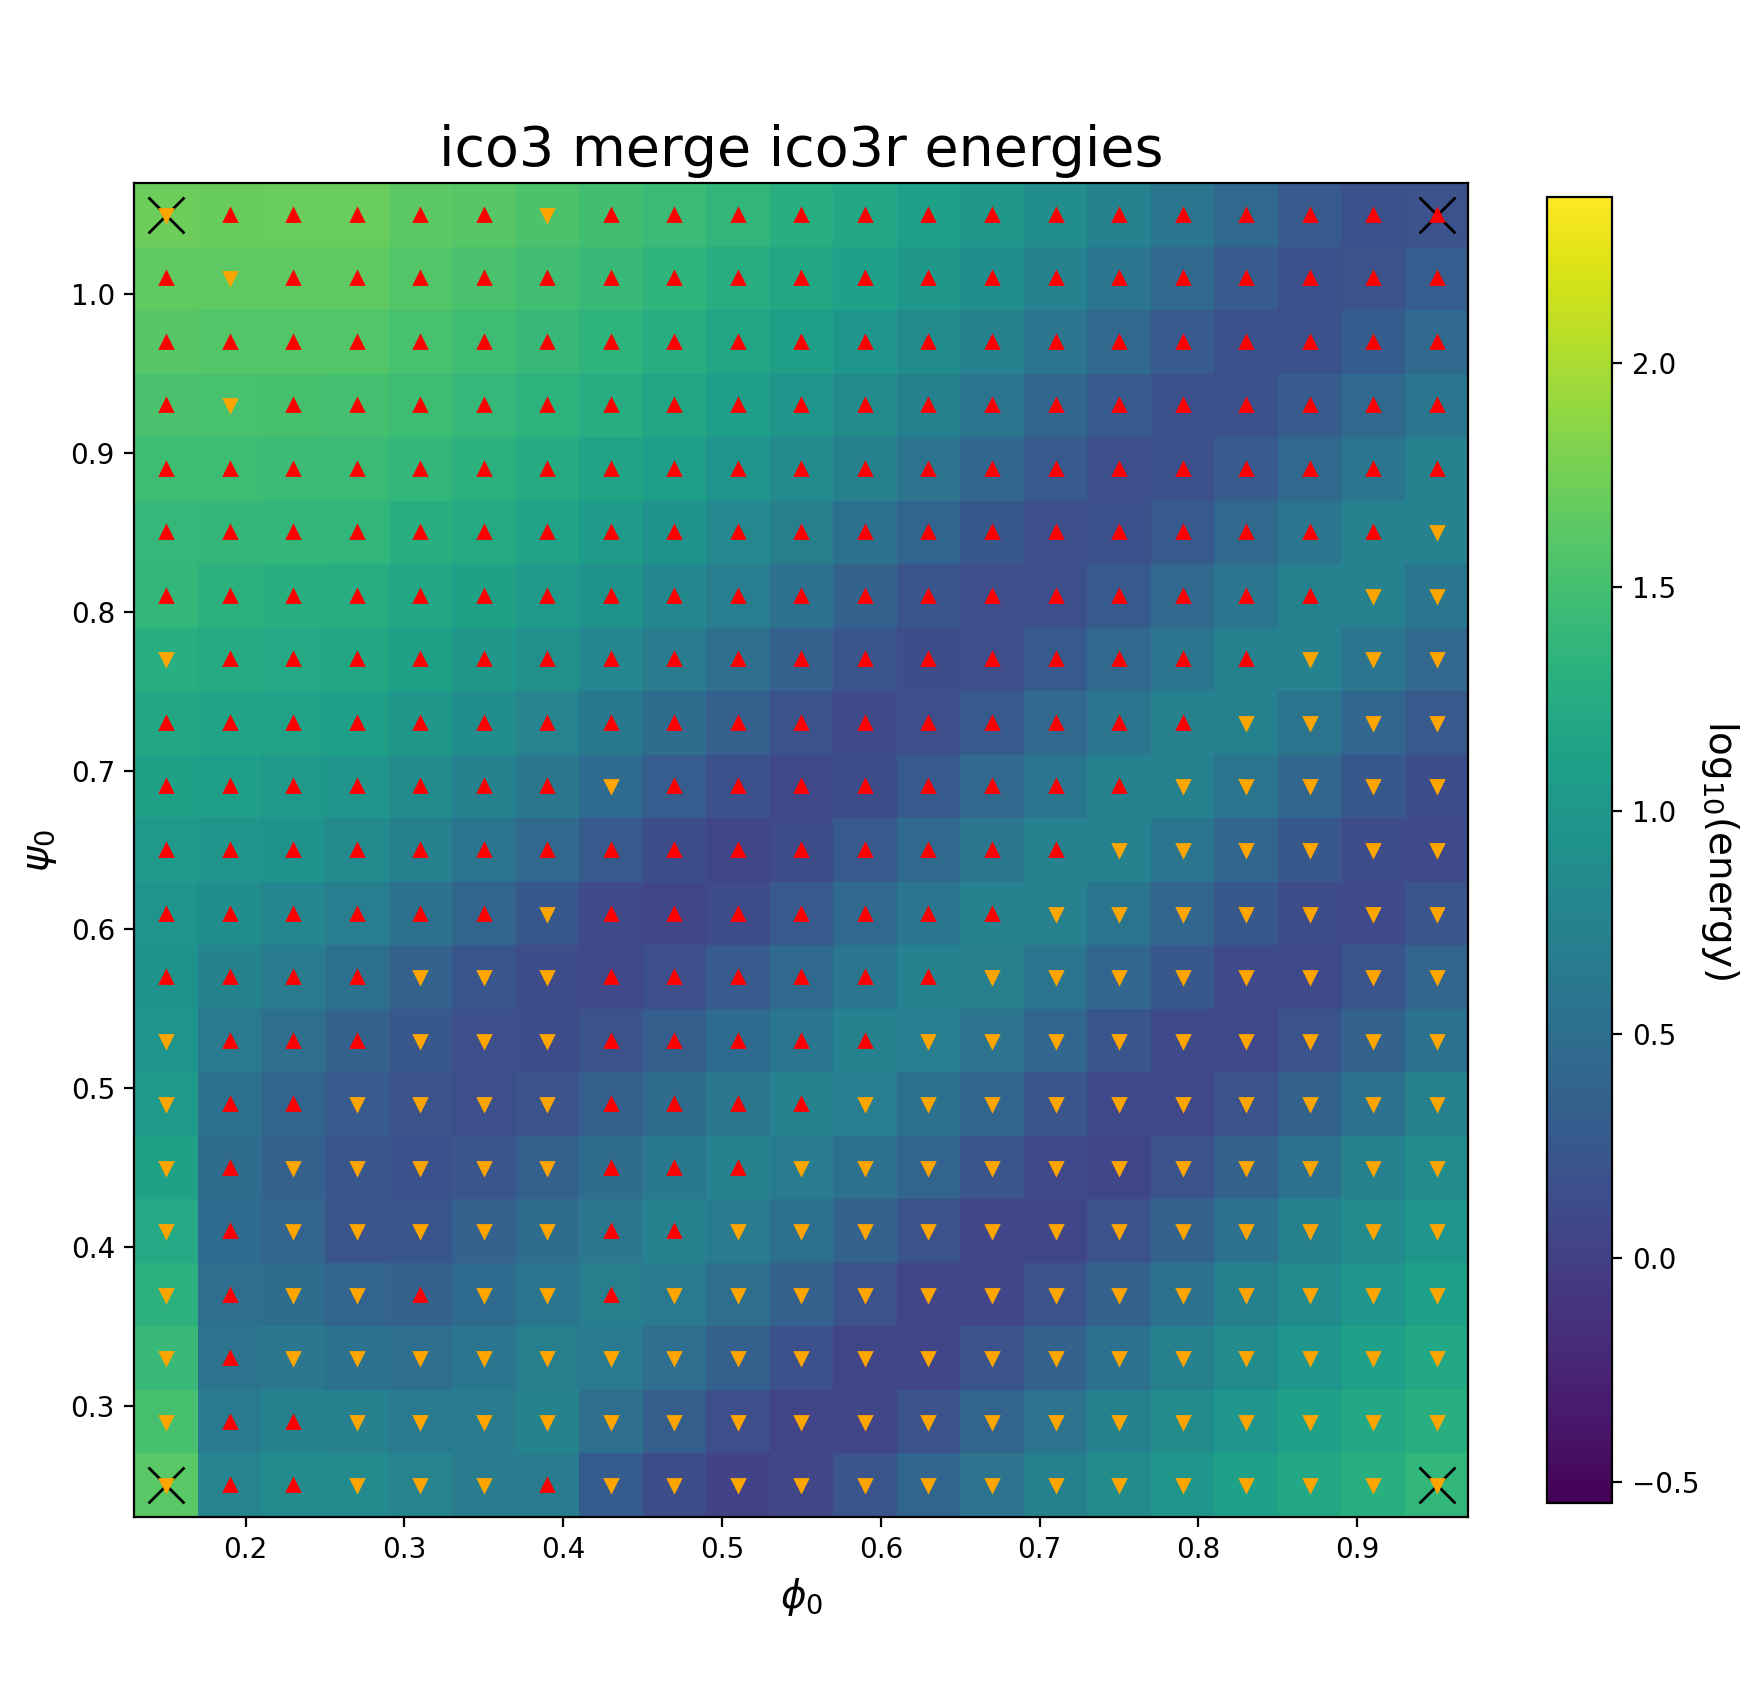
\includegraphics[height=\textheight]{landscape_merge.png}
	\caption[Combined energy landscape]{Minimum energies the two landscapes shown in \cref{fig:landscape_ico}. Values pulled from \cref{subfig:landscape_ico} are denoted with red dots and \cref{subfig:landscape_icor} with orange dots.}
	\label{fig:landscape_merge}
\end{figure}

Based on \cref{fig:landscape_merge}, we are equipped with a reasonable prediction to describe the inversion dynamics of \textit{C. flexa} sheets.
A flagella-in sheet at rest with equilibrium angles $\phi_{\text{in}}, \psi_{\text{in}}$ within the energy well of \cref{subfig:landscape_ico} that immediately changes equilibrium angles to $\phi_{\text{out}}, \psi_{\text{out}}$ may be constrained from inverting due to its collar-collar adhesions.
Despite this, the equilibrium angles are fixed as a result of environmental conditions and molecular action within the cells, and inversion relaxes the sheet to decrease energy into the higher yet still energetically preferable well of \cref{subfig:landscape_icor}. 

Despite the favorability of the flagella-out orientation in the active state, it is clear that there is a substantial energetic barrier to reach that state induced by collar-collar adhesion forces and collar stiffness. 
There is no evidence to suggest changing collar properties, so we are led to predict that changing cell sheet topology is the factor which enables inversion.

\mynote{collars might break some of their adhesion along their length but not all the way since they seem to be connected along the big length}



\begin{align*}
    \vec{F}_\gamma = \frac{\partial E}{\partial \vec{r}_\gamma} &= 2 \sum_{(\alpha, \rho)} \left( \phi_{(\alpha,\rho)} - \phi_0 \right) \frac{\partial \phi_{(\alpha,\rho)}}{\partial \vec{r}_\gamma} + 2 \sum_{(\alpha, \beta: \sigma, \rho)} \left( \psi(\hat{\bm{n}}_{\sigma\alpha\rho}, \hat{\bm{n}}_{\sigma\beta\rho}) - \psi_0 \right) \frac{\partial \psi_{(\alpha, \beta: \sigma, \rho)}}{\partial \vec{r}_\gamma} \\
    \frac{\partial \phi_{(\alpha,\rho)}}{\partial r_{\gamma i}} &= \frac{-1}{\sqrt{1 - (\hat{\bm{n}}_\alpha \cdot \hat{(\alpha\rho)})^2}} \left(\frac{\partial \hat{\bm{n}}_{\alpha j}}{\partial r_{\gamma i}} \hat{(\alpha\rho)}_j + \frac{\partial \hat{(\alpha\rho)}_j}{\partial r_{\gamma i}} \hat{\bm{n}}_{\alpha j} \right) \\
    \frac{\partial \hat{(\alpha\rho)}_j}{\partial r_{\gamma i}} &= \frac{(\delta_{\gamma\rho} - \delta_{\gamma\alpha})}{|r_\rho - r_\alpha|} \left( \delta_{ij} + \hat{(\alpha\rho)}_i\hat{(\alpha\rho)}_j \right) \\
    \frac{\partial \hat{\bm{n}}_{\alpha j}}{\partial r_{\gamma i}} &= \frac{\mathbb{1}_{\gamma\in \text{collars}(\alpha)} - n\delta_{\gamma\alpha}}{\left| \sum_{(\alpha, \rho)} (r_\rho - r_\alpha) \right|} \left(\delta_{ij} - \hat{\bm{n}}_{\alpha i} \hat{\bm{n}}_{\alpha j} \right) \\
    \frac{\partial \psi_{(\alpha, \beta: \sigma, \rho)}}{\partial r_{\gamma i}} &= \frac{-1}{\sqrt{1 - (\hat{\bm{n}}_{\rho\alpha\sigma} \cdot \hat{\bm{n}}_{\rho\beta\sigma}})^2} \left(\frac{\partial \hat{\bm{n}}_{\rho\alpha\sigma j}}{\partial r_{\gamma i}} \hat{\bm{n}}_{\rho\beta\sigma j} + \frac{\partial \hat{\bm{n}}_{\rho\beta\sigma j}}{\partial r_{\gamma i}} \hat{\bm{n}}_{\rho\alpha\sigma j} \right) \\
    \frac{\partial \hat{\bm{n}}_{\rho\alpha\sigma j}}{\partial r_{\gamma i}} &= \text{too big see notes}
\end{align*}
\section{Everything before written}
\section{Discrete surface model}
\subsection{How to define the surface}

We need to determine what parts of our physical problem we will keep track of, and how we will use them to define an energy. There are two natural, physical planar graphs to look at. We could either form the graph with cell bodies forming vertices and edges defined by cells whose collars make contact with each other. Alternatively, vertices could be represented by places where two cells' collars lose contact with each other, and edges could be along the line where those collars contact. 

Since these graphs are planar (albeit not necessarily lying along a physical plane), we have a well-defined notion of a graph dual, where each face in one graph corresponds to a vertex in the other. What we find is that the two graphs described above are dual to each other (Figure \ref{subfig:duals1}). One graph specifies the topology of the other, but we are considering these as spatial graphs to use their geometries so our problem is not so simple. Knowing the positions of all vertices and knowing the edges of one graph does not give complete information about the other.

Since each cell is identical, we might imagine that the distances between two cells and their mutual boundary is equal. In a loose sense, then, their interactions form a Voronoi tesselation on the surface of collar interactions (with respect to the metric on that surface). We can then take the dual to know that the graph of cell bodies is triangulated, as the dual of a Voronoi tesselation is a Delaunay triangulation (Figure \ref{subfig:duals2}).

\begin{figure}[htbp]
    \centering
    \begin{subfigure}[b]{0.52\textwidth}
        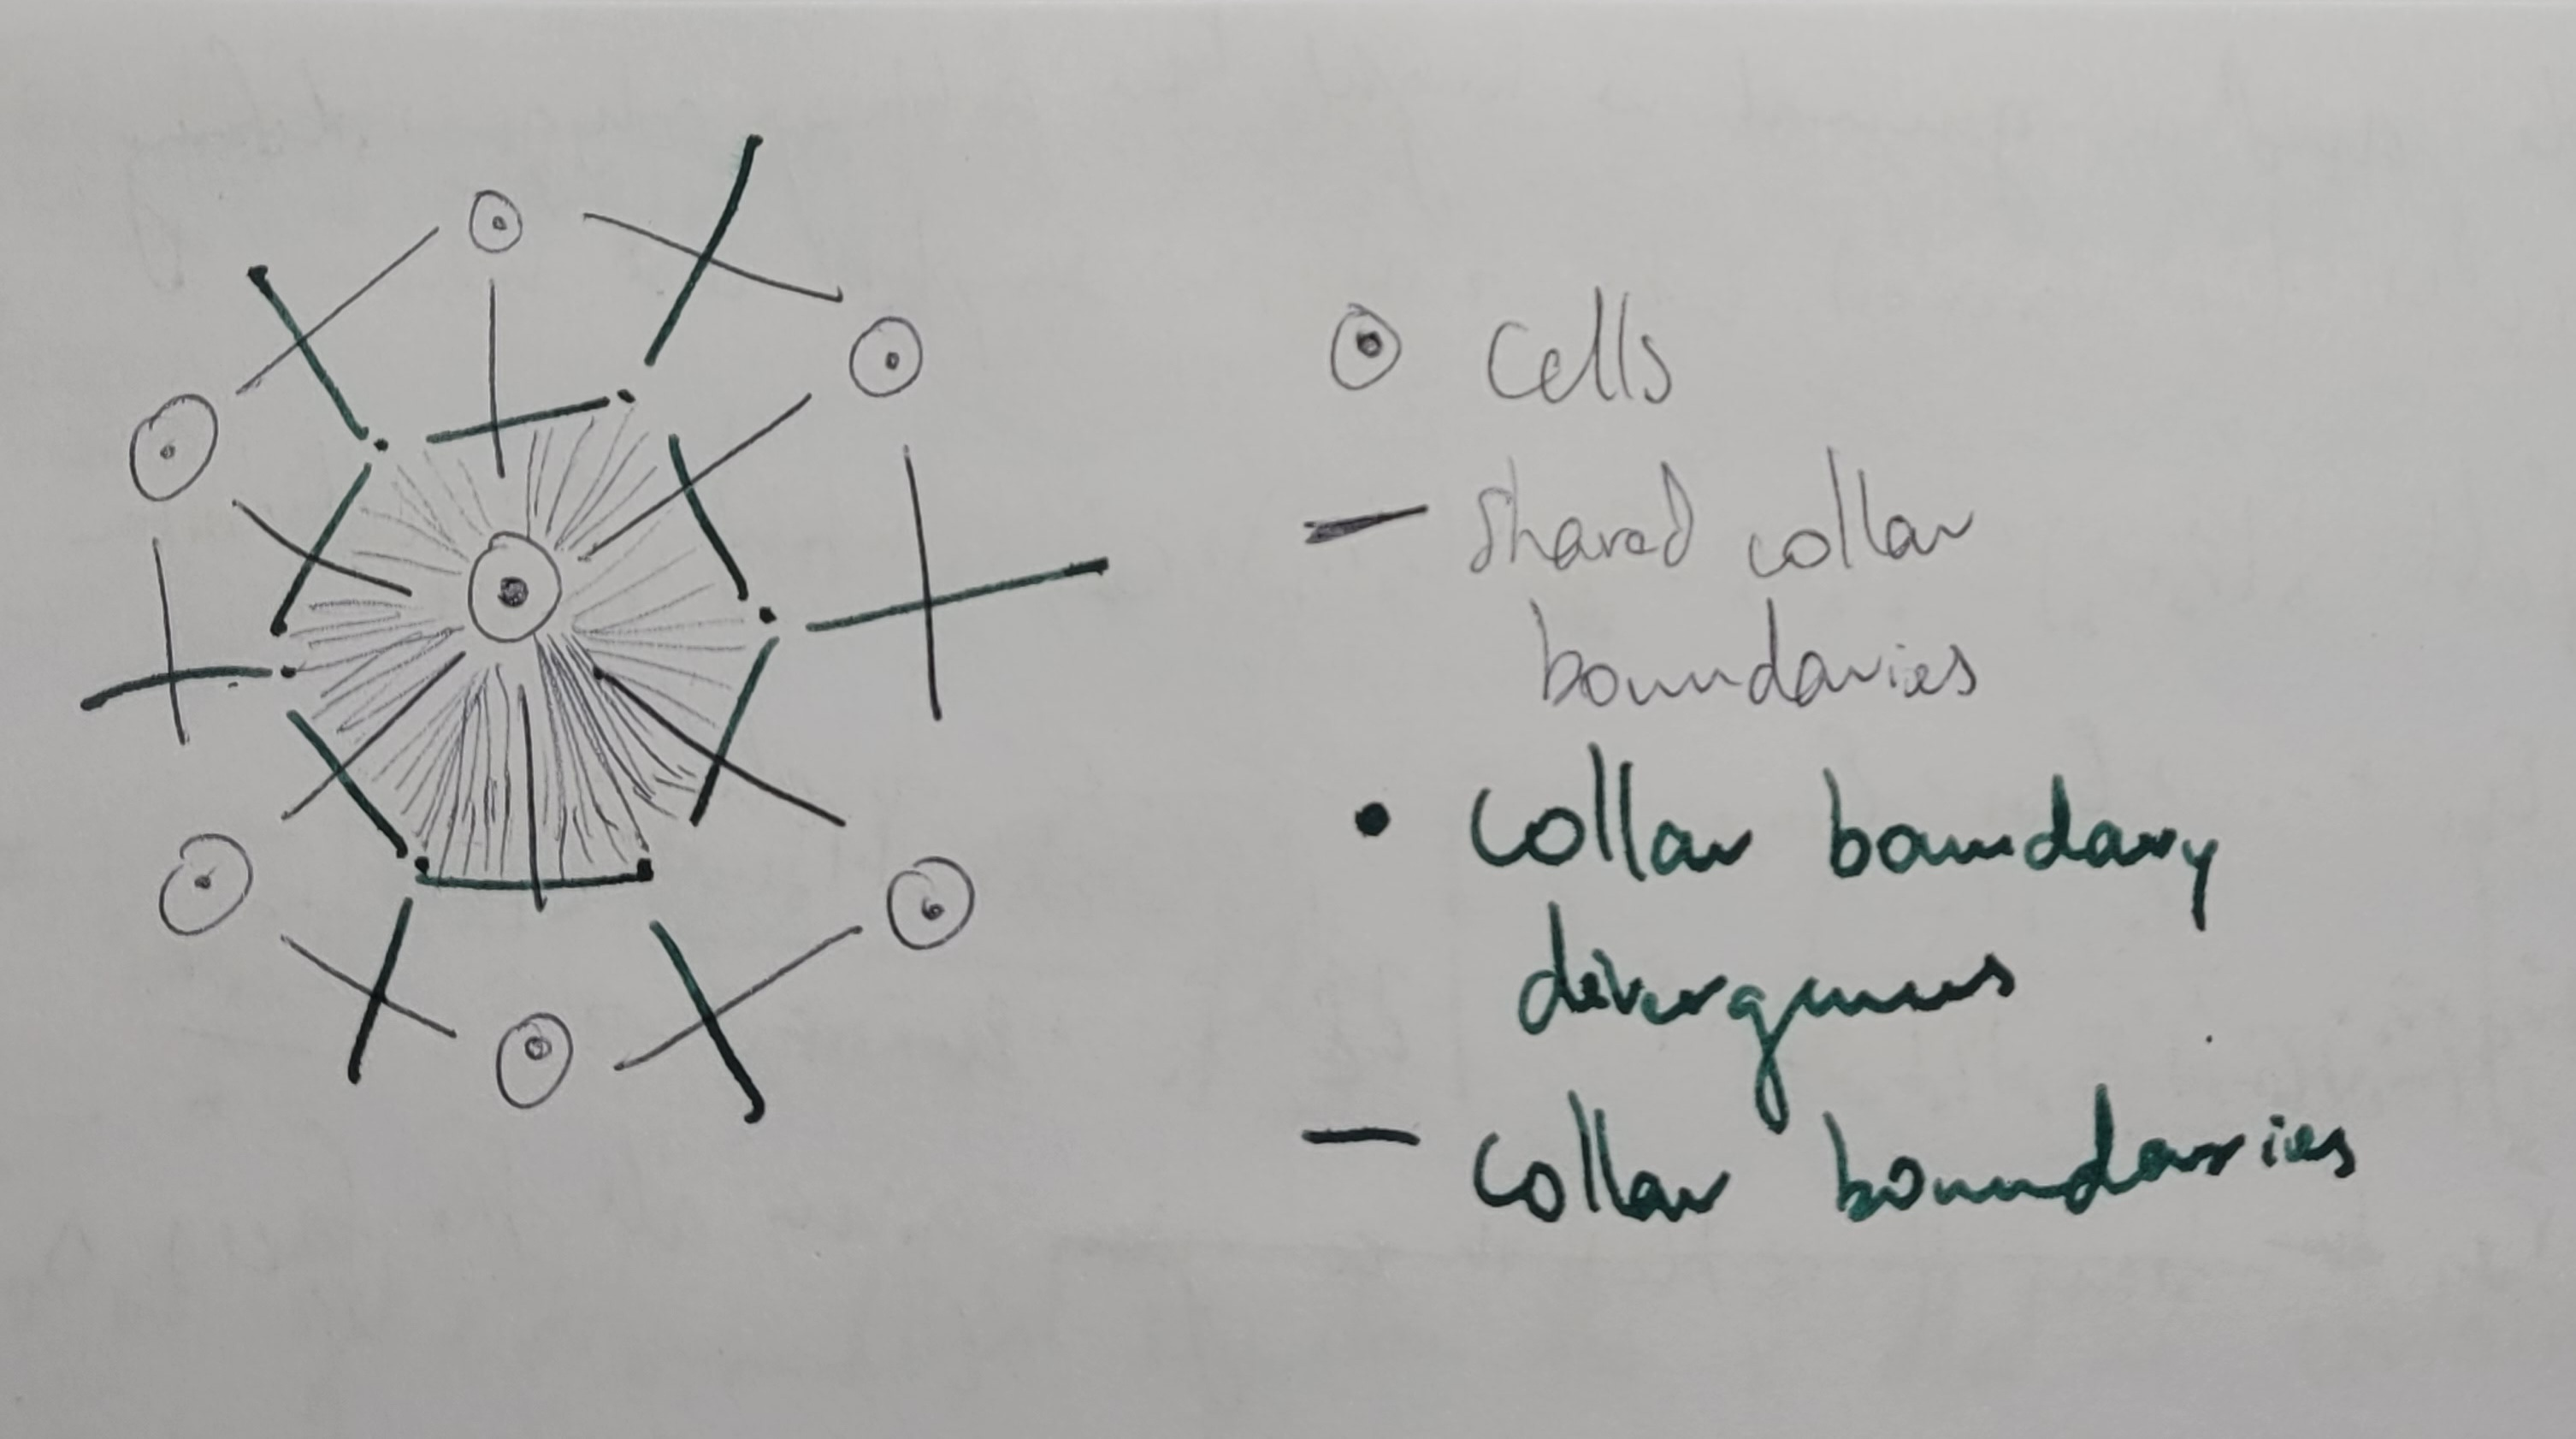
\includegraphics[width=\textwidth]{duals1.jpg}
        \caption{}
        \label{subfig:duals1}
    \end{subfigure}
    ~
    \begin{subfigure}[b]{0.46\textwidth}
        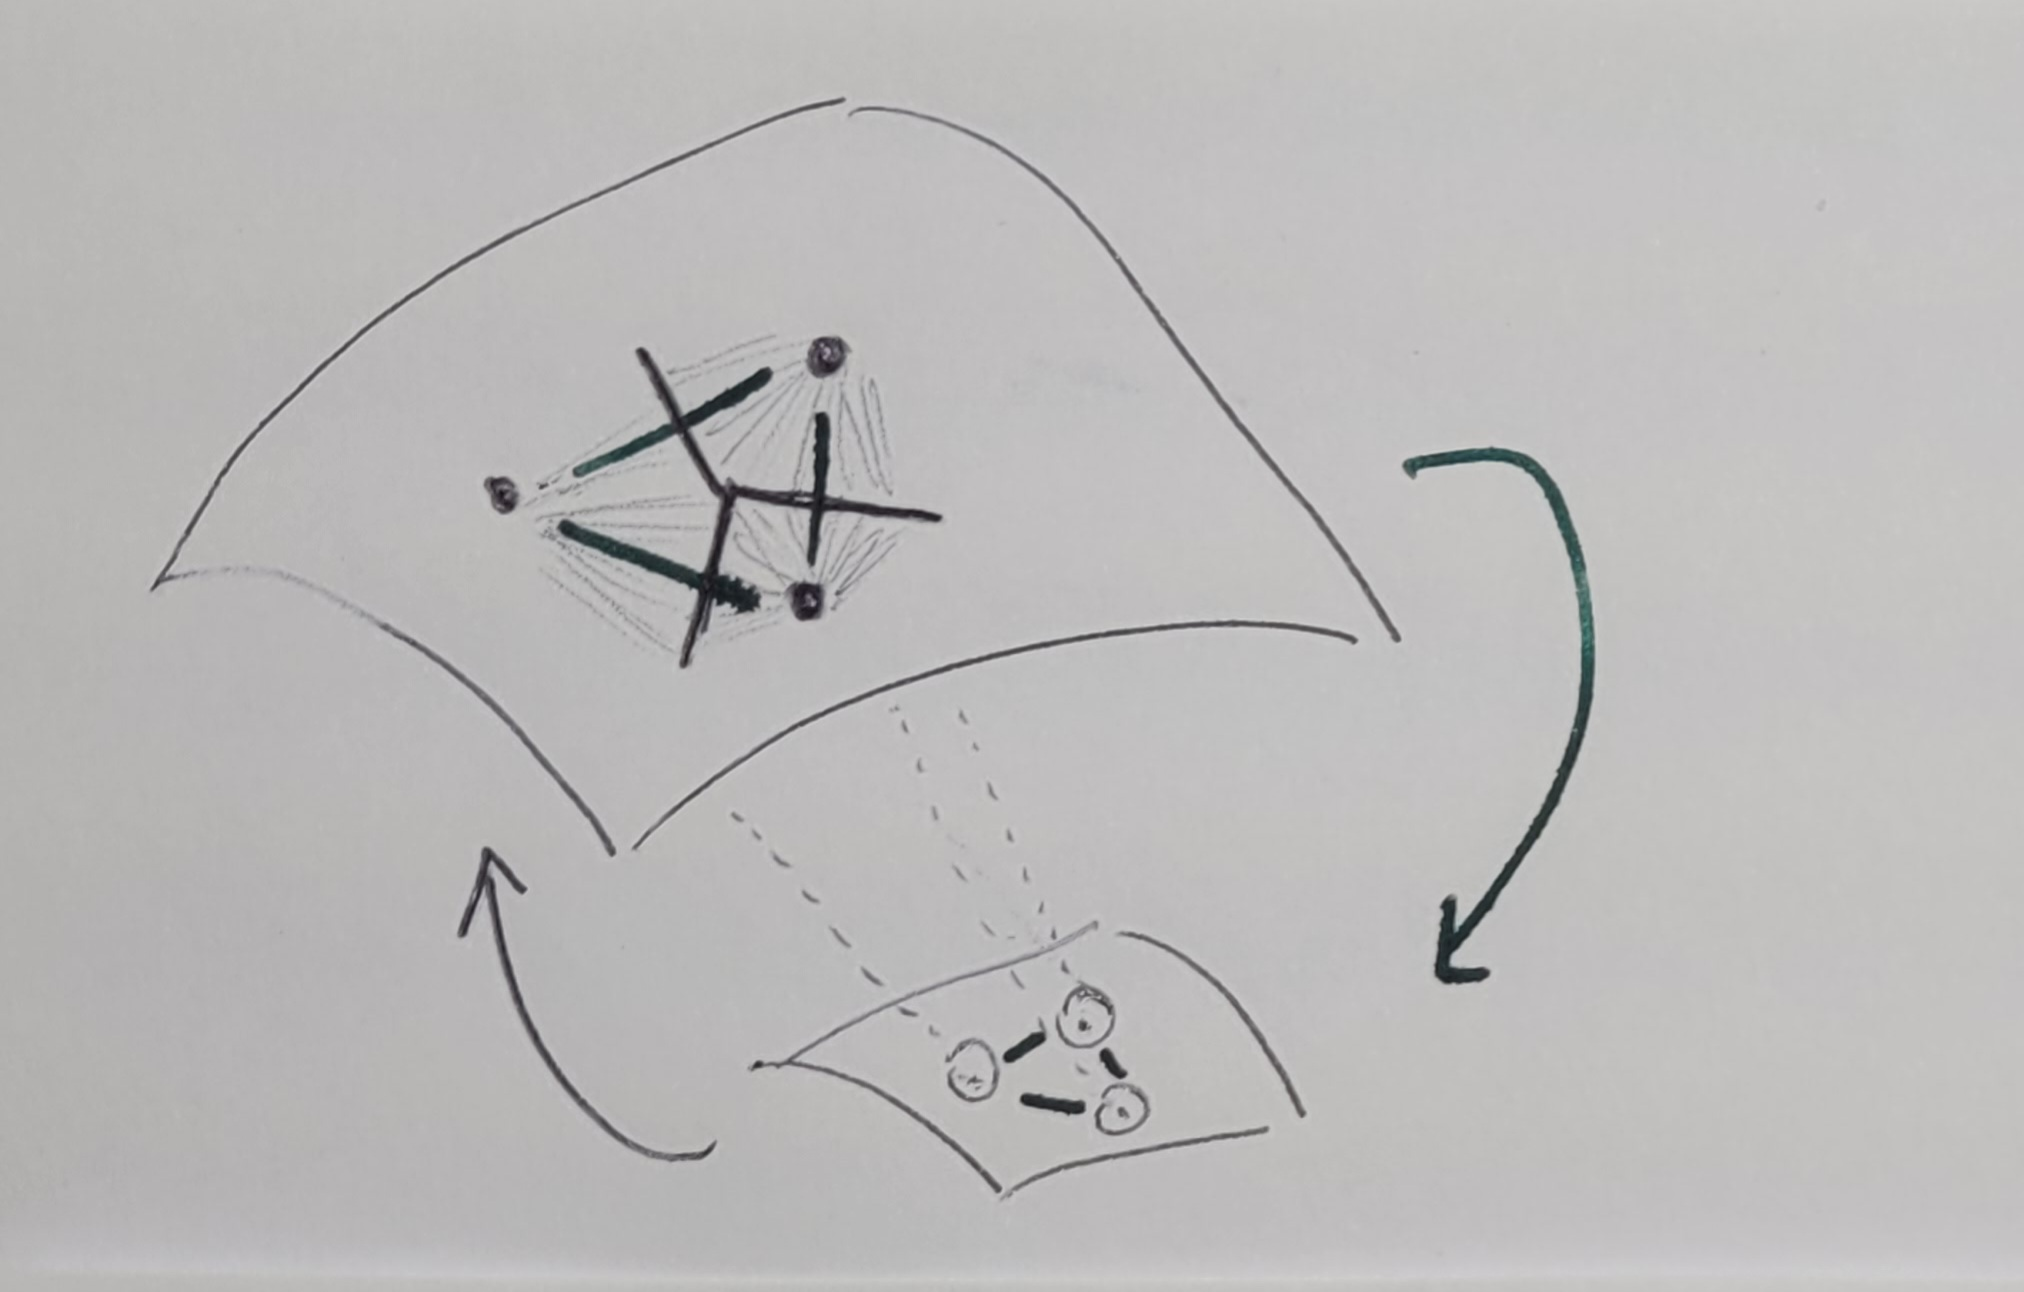
\includegraphics[width=\textwidth]{duals2.jpg}
        \caption{}
        \label{subfig:duals2}
    \end{subfigure}
    \caption{Two views of the physical dual graphs used in describing \textit{C. flexa}.}
    \label{fig:duals}
\end{figure}

\subsection{Surface formed by collar boundaries}
\subsubsection{Stretching}

The physical interactions happen at the collar boundaries, so it makes sense to define energy based on the graph that quantifies them. If two cells have a collar boundary described by $\bm{r_a} t + (1-t)\bm{r_b}$ with $0 \leq t \leq 1$ and the energy is defined by continuously many springs from the boundary to a projected cell point $\bm{r_\Delta}$, then the energy $\e_{ab}$ of that boundary is 

\begin{align}
    \e_{ab} = \int_0^1 \left[(\bm{r_a}t + (1-t)\bm{r_b}) - \bm{r_\Delta} \right]^2 dt &= \frac{1}{3} (\bm{r_a} + \bm{r_b})^2 - \frac{1}{3} \bm{r_a}\cdot\bm{r_b} - \bm{r_\Delta} \cdot (\bm{r_a} + \bm{r_b}) + \bm{r_\Delta}^2. \label{eq:eab}
\end{align}

The energy corresponding to a cell consists of the line energies of all the collar interfaces. We find the position $\bm{r_\Delta}$ by setting the gradient of equation \ref{eq:eab} with respect to $\bm{r_\Delta}$ to zero for all lines $ab$. If $b$ indexes the vertices that cell $\Delta$ has, then 

\begin{align*}
    0 = \frac{d\e}{d\bm{r_\Delta}} &= -\sum_{b\in\Delta} \bm{r_b} + 2n\bm{r_\Delta} \\
    \bm{r_\Delta} &= \frac{1}{n} \sum_{b\in\Delta} \bm{r_b}.
\end{align*}

The force on vertex $a$ is then given by the gradient of the whole sheet energy $\e_{\text{sheet}}$, which is the sum of the energies $\e_\Delta$ corresponding to each cell $\Delta$. 

\begin{align*}
    \frac{d \e_{\text{sheet}}}{d\bm{r_a}} &= \frac{d}{d\bm{r_a}} \sum_\Delta \e_\Delta = \sum_{\Delta:a \in \Delta} \frac{d\e_\Delta}{d\bm{r_a}} = \sum_{\Delta:a\in\Delta} \frac{d}{d\bm{r_a}} \sum_{b \in \Delta} (\bm{r_b} - \bm{r_\Delta})^2. \\
    \intertext{Since $\bm{r_\Delta}$ depends on $\bm{r_a}$ itself, we write} \\
    \bm{f_{\text{on }a}} &= -\sum_{\Delta:a\in\Delta} \frac{d}{d\bm{r_a}} \sum_{b \in \Delta} \left(\bm{r_b} - \frac{1}{n} \sum_{c\in\Delta} \bm{r_c} \right)^2 \\
    &= \sum_{\Delta:a\in\Delta} \sum_{b \in \Delta} \left(2\bm{r_a}\delta_{ab} - \frac{2}{n} \sum_{c\in\Delta}\left(\bm{r_c}\delta_{ab} + \bm{r_b}\delta_{ac}\right) + \frac{1}{n^2} \sum_{c\in\Delta}\sum_{d\in\Delta} \left(\delta_{ac}\bm{r_d} + \delta_{ad}\bm{r_c} \right) \right) \\
    &= -2\left(\bm{r_a} - \bm{r_\Delta} \right)
\end{align*}

This process was overkill, since we could have reasonably assumed that $\bm{r_\Delta}$ would be at the vertices' center of mass and that we'd effectively get springs from $\bm{r_\Delta}$ to each vertex. This is thanks to linearity of the collar springs. However, assuming that the collars have a positive equilibrium length $r_0$ makes it necessary to go through the above procedure.

If instead the line energy is 

\begin{align*}
    \e_{ab} &= \int_0^1 \left(\left|\bm{r_a}t + (1-t)\bm{r_b} - \bm{r_\Delta}\right| - r_0 \right)^2 dt, \\
    \intertext{then the cell position $\bm{r_\Delta}$ is the solution to} \\
    0 &= -2 \sum_{b\in\Delta} \bm{r_b} + 6 \bm{r_\Delta} - 2r_0 \frac{d}{d\bm{r_\Delta}} \sum_{(b,c) \text{ edge in }\Delta} \int_0^1 \left| \bm{r_b}t - (1-t)\bm{r_c} - \bm{r_\Delta} \right| dt \\
    0 &= -2 \sum_{b\in\Delta} \bm{r_b} + 6 \bm{r_\Delta} - 2r_0 \sum_{(b,c)} \int_0^1 \frac{\bm{r_\Delta} - \bm{r_c} - t(\bm{r_b} - \bm{r_c})}{\left|\bm{r_b}t - (1-t)\bm{r_c} - \bm{r_\Delta} \right|} dt.
\end{align*}

We can actually evaluate the integral above, but I found that it gives a transcendental equation for $\bm{r_\Delta}$ and decided it wasn't pursuing further on paper. Nonzero equilibrium length springs is better pursued numerically. Alternatively, we simply define springs from $\bm{r_\Delta}$ to each dual graph vertex rather than making the collars consist of continuous springs.

\subsubsection{Bending}

One way to define a bending energy is to give each cell a vector that corresponds to the midline pointing out from the center of the cell, which I have implicitly drawn in the figures of individuals flexas. From there, we could reasonably define a bending energy from the interactions between two interacting flexas by the angle between their corresponding ``normal'' vectors weighted by the length of their interface. 

Defining an individual vector is made complicated by the fact that the vertices along the cycles corresponding to each flexa are not necessarily coplanar, provided that a given cell is interacting with more than three other cells. One option, although I have not developed it, is to find the plane whose summed mean squared distances to each vertex for a cell is minimised. It would possibly be more accurate to again treat the edges as lines and minimise the integrated distance from the normal plane to the edges. Either way, the energy dictated by the angle between adjacent normal vectors will need to be summed over all pairs of neighboring cells, namely all edges in the graph where edges correspond to cell neighbors (not collar interfaces).

\subsection{Surface formed by cell bodies}

The graph of cell bodies and neighbor edges makes it easy to work with springs, but it is less clear how to define a bending energy. The math for springs is identical to previously, so let's just think about how to define bending energy.

\mynote{needs more work}

% \subsubsection{Bending}

\section{Including both cells and collar boundaries}

\subsection{Initial sheet}

\subsection{Numerical optimisation routine} \label{subsec:numerical}

Finally, we numerically optimise. I changed $\phi_0$ to be defined relative to the initial value of $\phi$, and likewise for $\psi$. If we make $\phi_0$ smaller and $\psi_0$ larger, we expect the cell collars to contract and for cell-cell distances to lengthen. In other words, we expect the sheet to curve upward, so that the cells on the edges go in the direction that the collars are.

The numerical optimisation problem gives a clean sensible solution, which is shown projected onto the $xy$-plane in Figure \ref{fig:layout_curved}. We can tell that the sheet is curved just looking at this alone, which is a massive relief and confirmation of what we expect.

\begin{figure}[htbp]
    \centering
    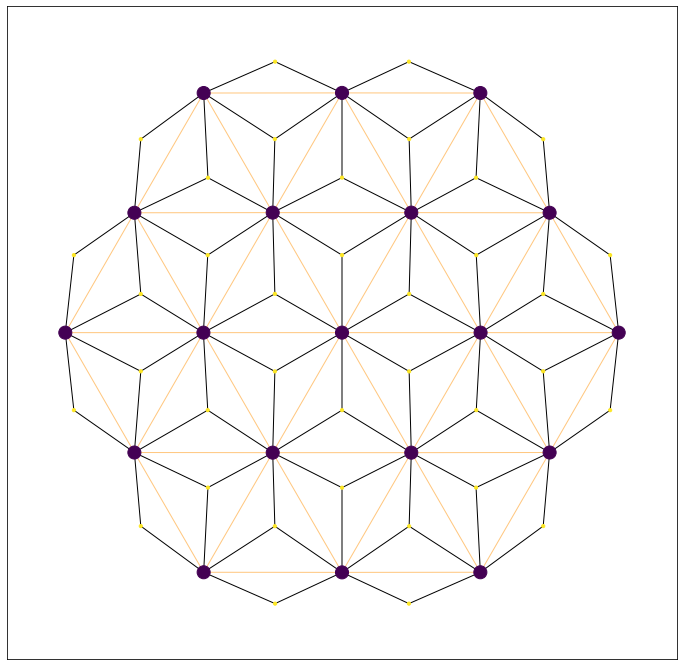
\includegraphics[width=0.8\textwidth]{layout_curved.png}
    \caption{Figure in the same style of Figure \ref{fig:layout_init} showing the cell sheet projected onto the $xy$-plane after minimising energy. }
    \label{fig:layout_curved}
\end{figure}

The solution in Figure \ref{fig:layout_curved} is for $\phi_0 = 0.99 \phi_{\text{init}}$ and $\phi_0 = 1.03 \psi_{\text{init}}$, where $\phi_{\text{init}}$ and $\psi_{\text{init}}$ are the initial angles in the flat sheet state. We could now bask in the glory of our solution and look at it in 3d (Figure \ref{subfig:shallow}).

The resulting structure is really pretty sensitive to small changes in $\phi_0, \psi_0$. Figure \ref{subfig:deep} shows the structure that comes out of $\phi_0 = 0.9 \phi_{\text{init}}$, $\psi_0 = 1.15\psi_{\text{init}}$. 

\begin{figure}[htbp]
    \centering
    \begin{subfigure}[b]{\textwidth}
        \centering 
        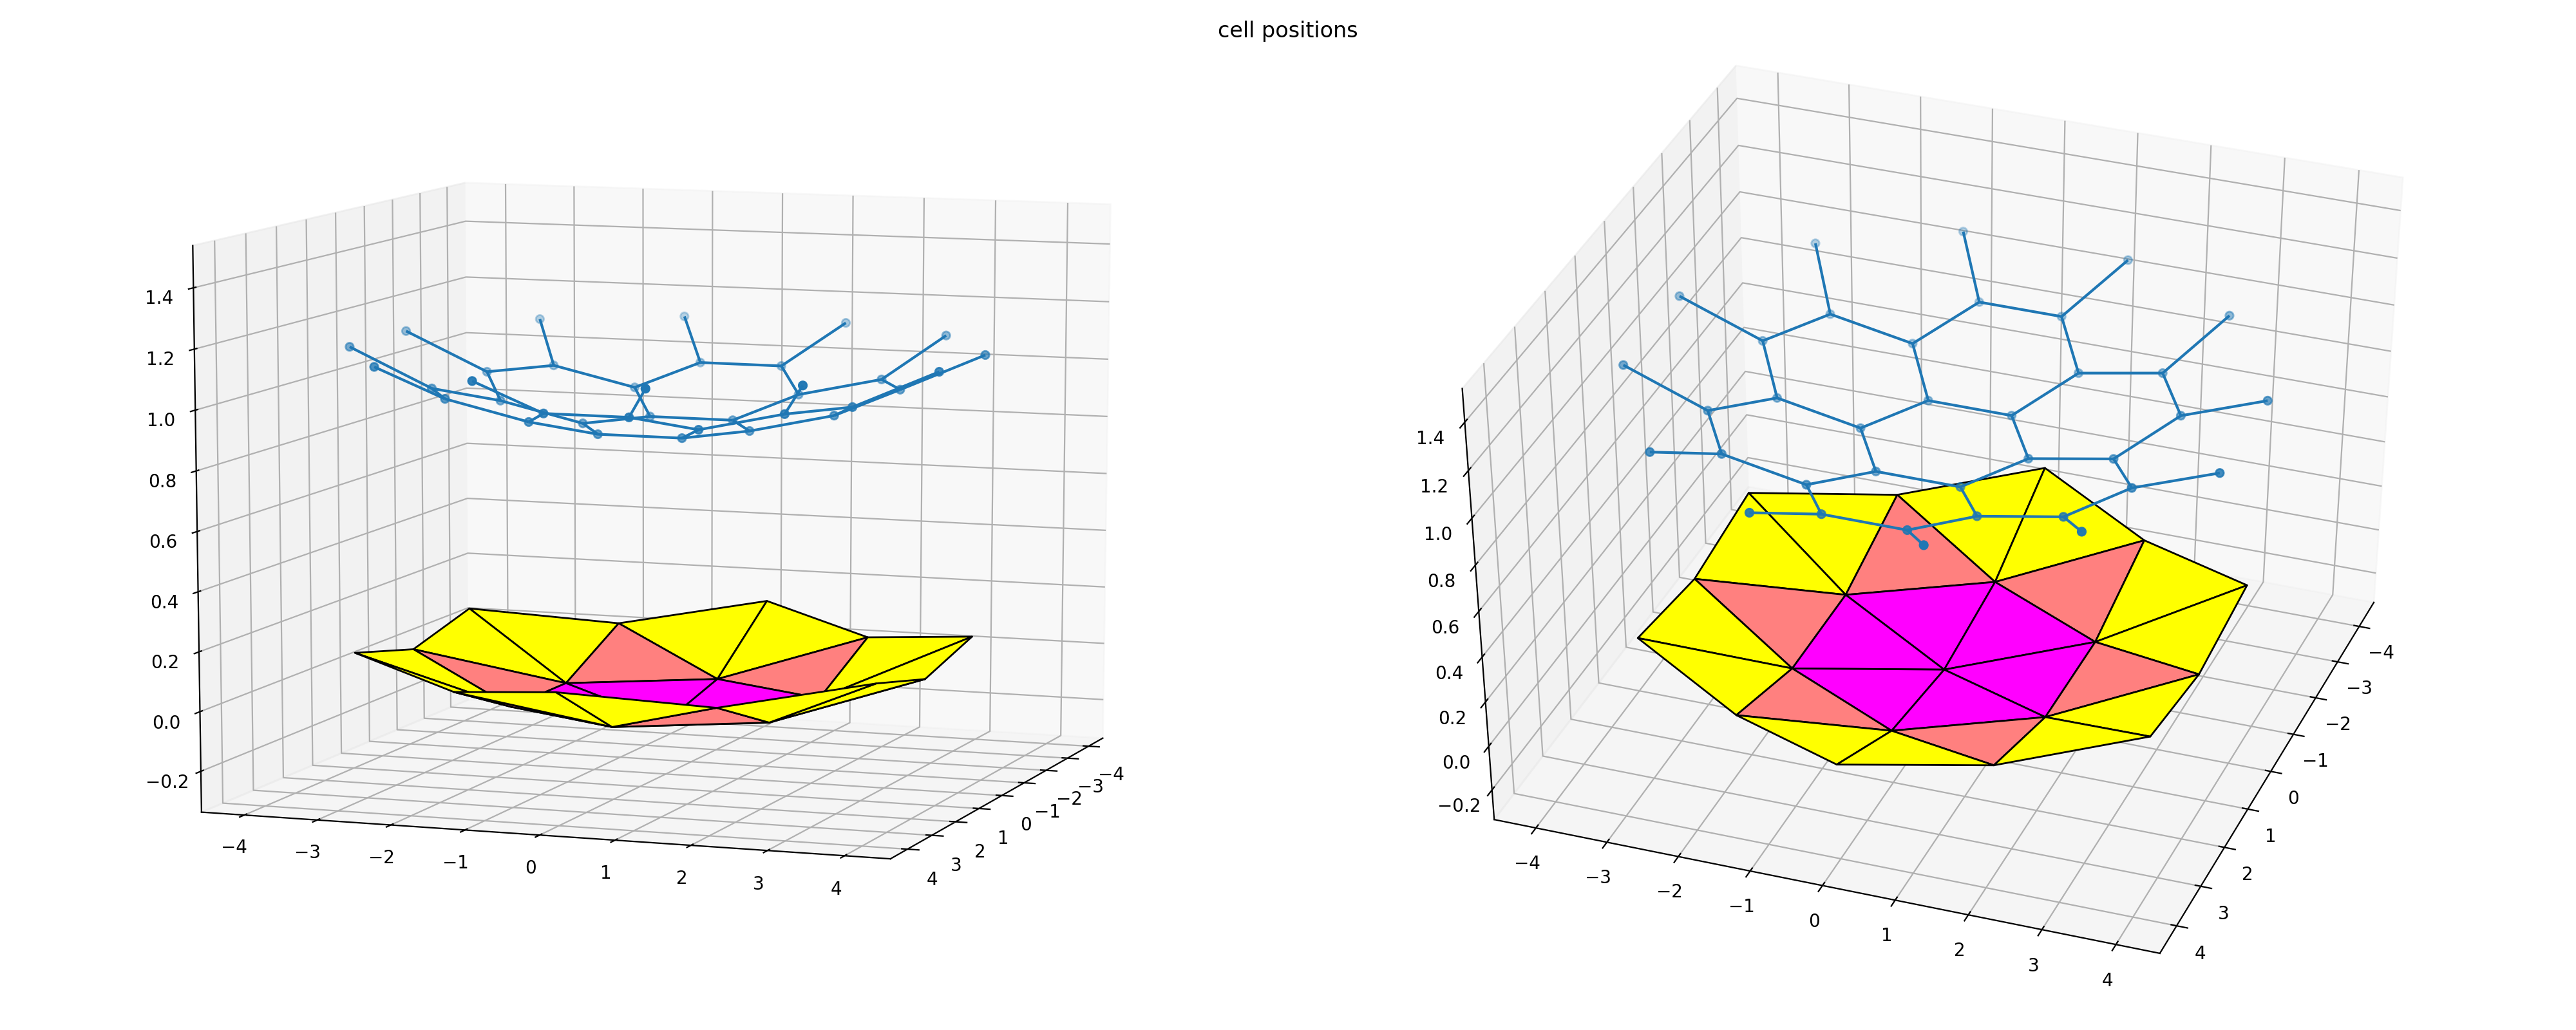
\includegraphics[width=\textwidth]{shallow.png}
        \caption{}
        \label{subfig:shallow}
    \end{subfigure}
    \begin{subfigure}[b]{\textwidth}
        \centering
        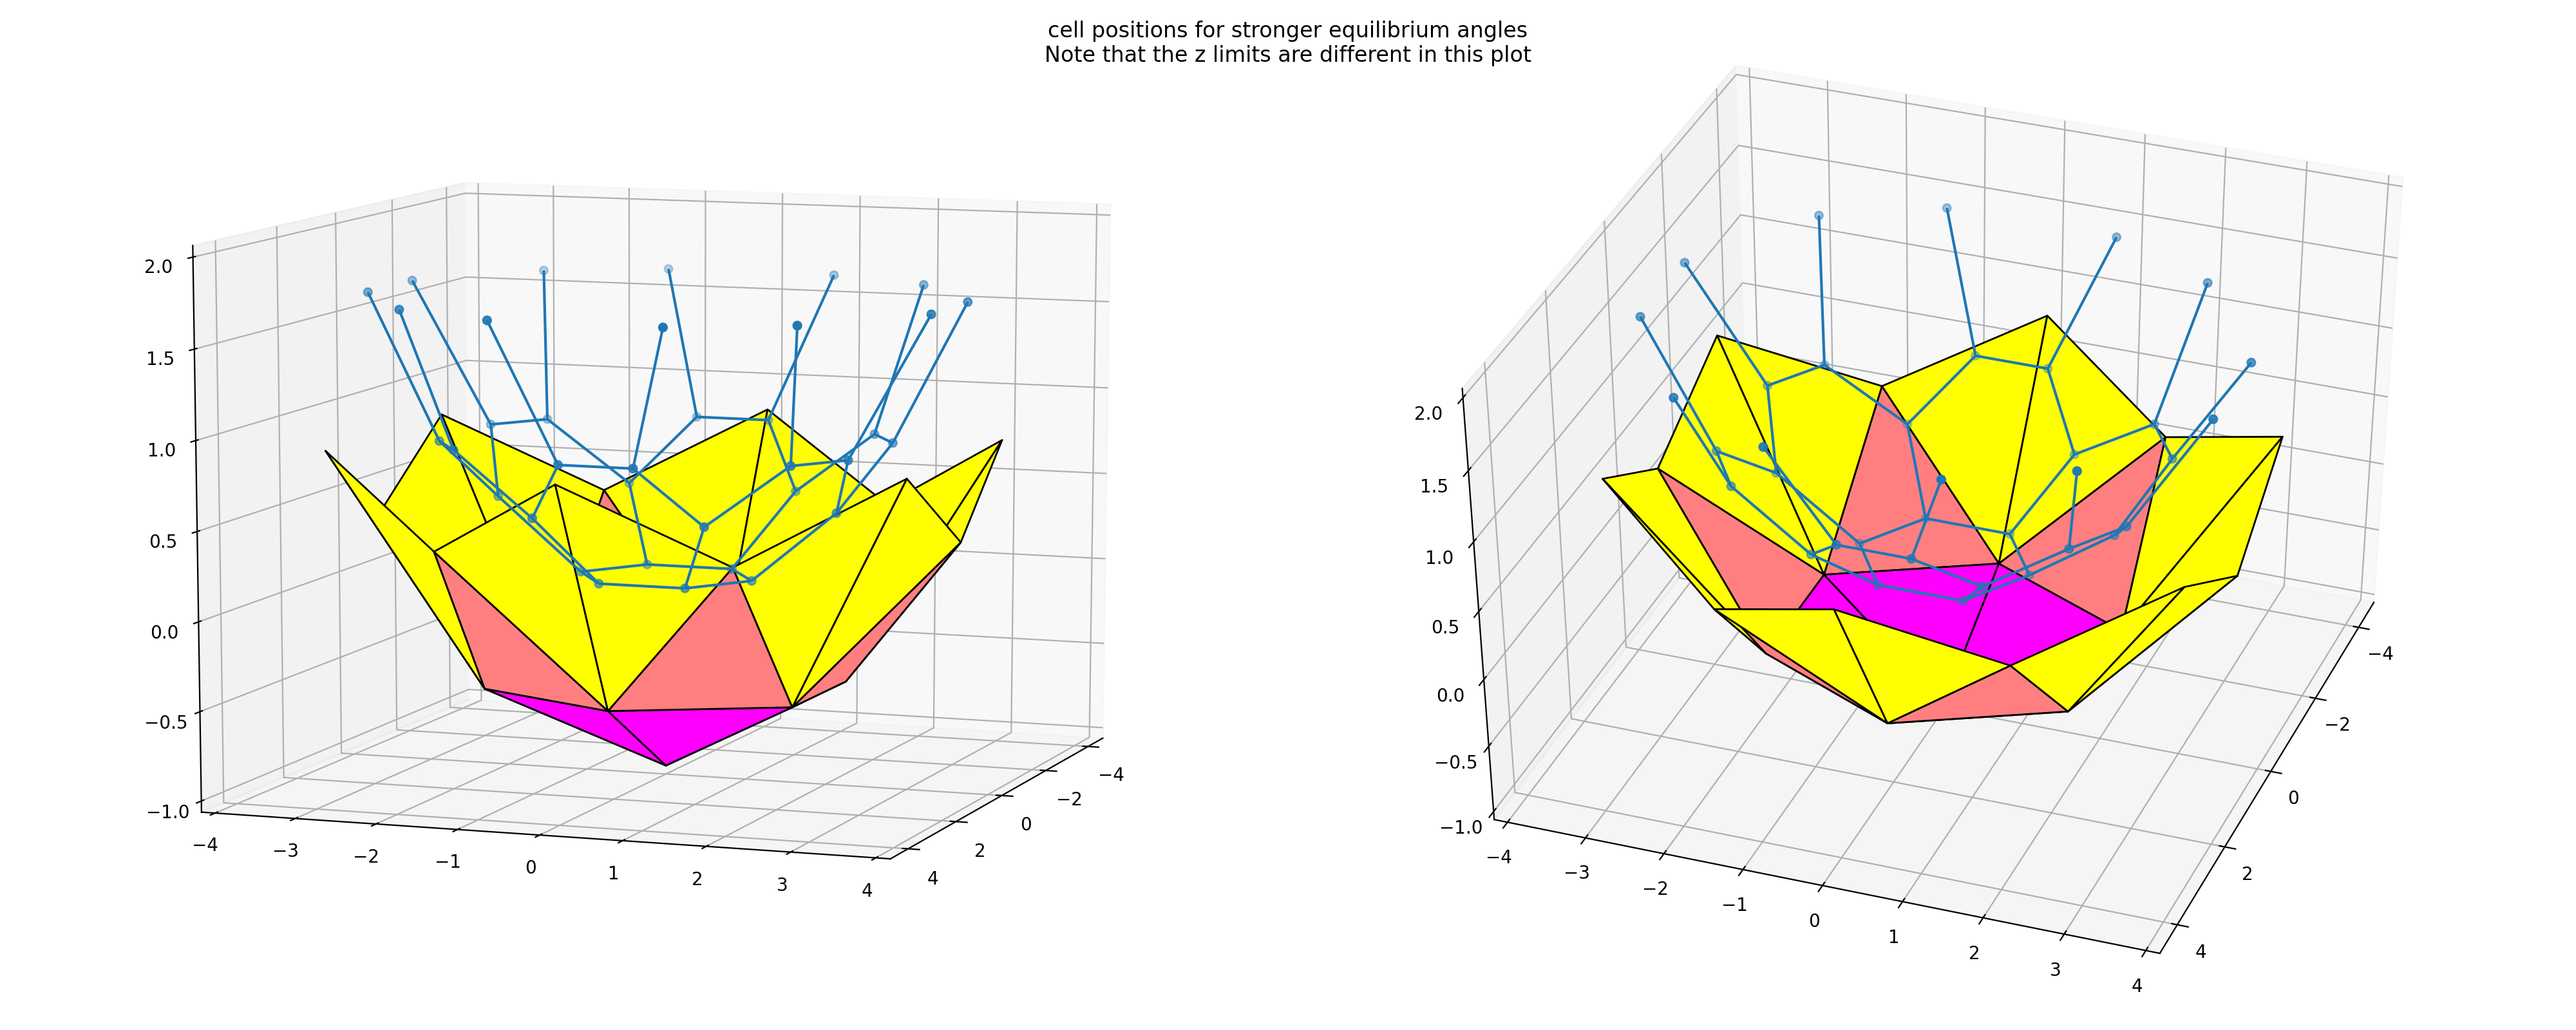
\includegraphics[width=\textwidth]{deep.png}
        \caption{3d projections of the curved sheet formed by $\phi_0 = 0.9 \phi_{\text{init}}$, $\psi_0 = 1.15\psi_{\text{init}}$. }
        \label{subfig:deep}
    \end{subfigure}
    \caption{Cell sheet geometry from the hexagonal lattice in Figure \ref{fig:layout_init} and parameters (\ref{subfig:shallow}) $\phi_0 = 0.99 \phi_{\text{init}}$, $\phi_0 = 1.03 \psi_{\text{init}}$, $\ell_0 = \ell_{\text{init}}=1.52$, (\ref{subfig:deep}) $\phi_0 = 0.9 \phi_{\text{init}}$, $\psi_0 = 1.15\psi_{\text{init}}$, $\ell_0 = \ell_{\text{init}}=1.52$. }
\end{figure}

\subsection{Topology}

In section \ref{subsubsec:flat}, I mentioned that the flat sheet is a stable minimum. But it is here because the lattice is regular. A single pentagon in a hexagonal lattice (like a football (soccer) ball, thanks Lloyd) will make it so no $\phi_0$ and $\psi_0$ will make every cell make the other cells flat. 

What I think is interesting about this is the connection between graph topology and surface geometry. I think, in a continuous sense, graph topology affects Gaussian curvature through the energy function. 

\subsubsection{Adding noise to initial cell positions in Figure \ref{fig:layout_init}}

We expect the initial lattice in Figure \ref{fig:layout_init} to produce a sheet with 6-fold symmetry. Since the graph of connections is produced by a Voronoi tessellation, small changes to initial boundary cell positions can change the graph topology for boundary cells. 

When adding noise to the initial cell positions, the change in topology at some boundary nodes results in substantial effects felt over the sheet. Figure \ref{fig:hexnoise} shows the effect of different topology at the boundary.

\begin{figure}[htbp]
    \centering
    \begin{subfigure}[b]{\textwidth}
        \centering
        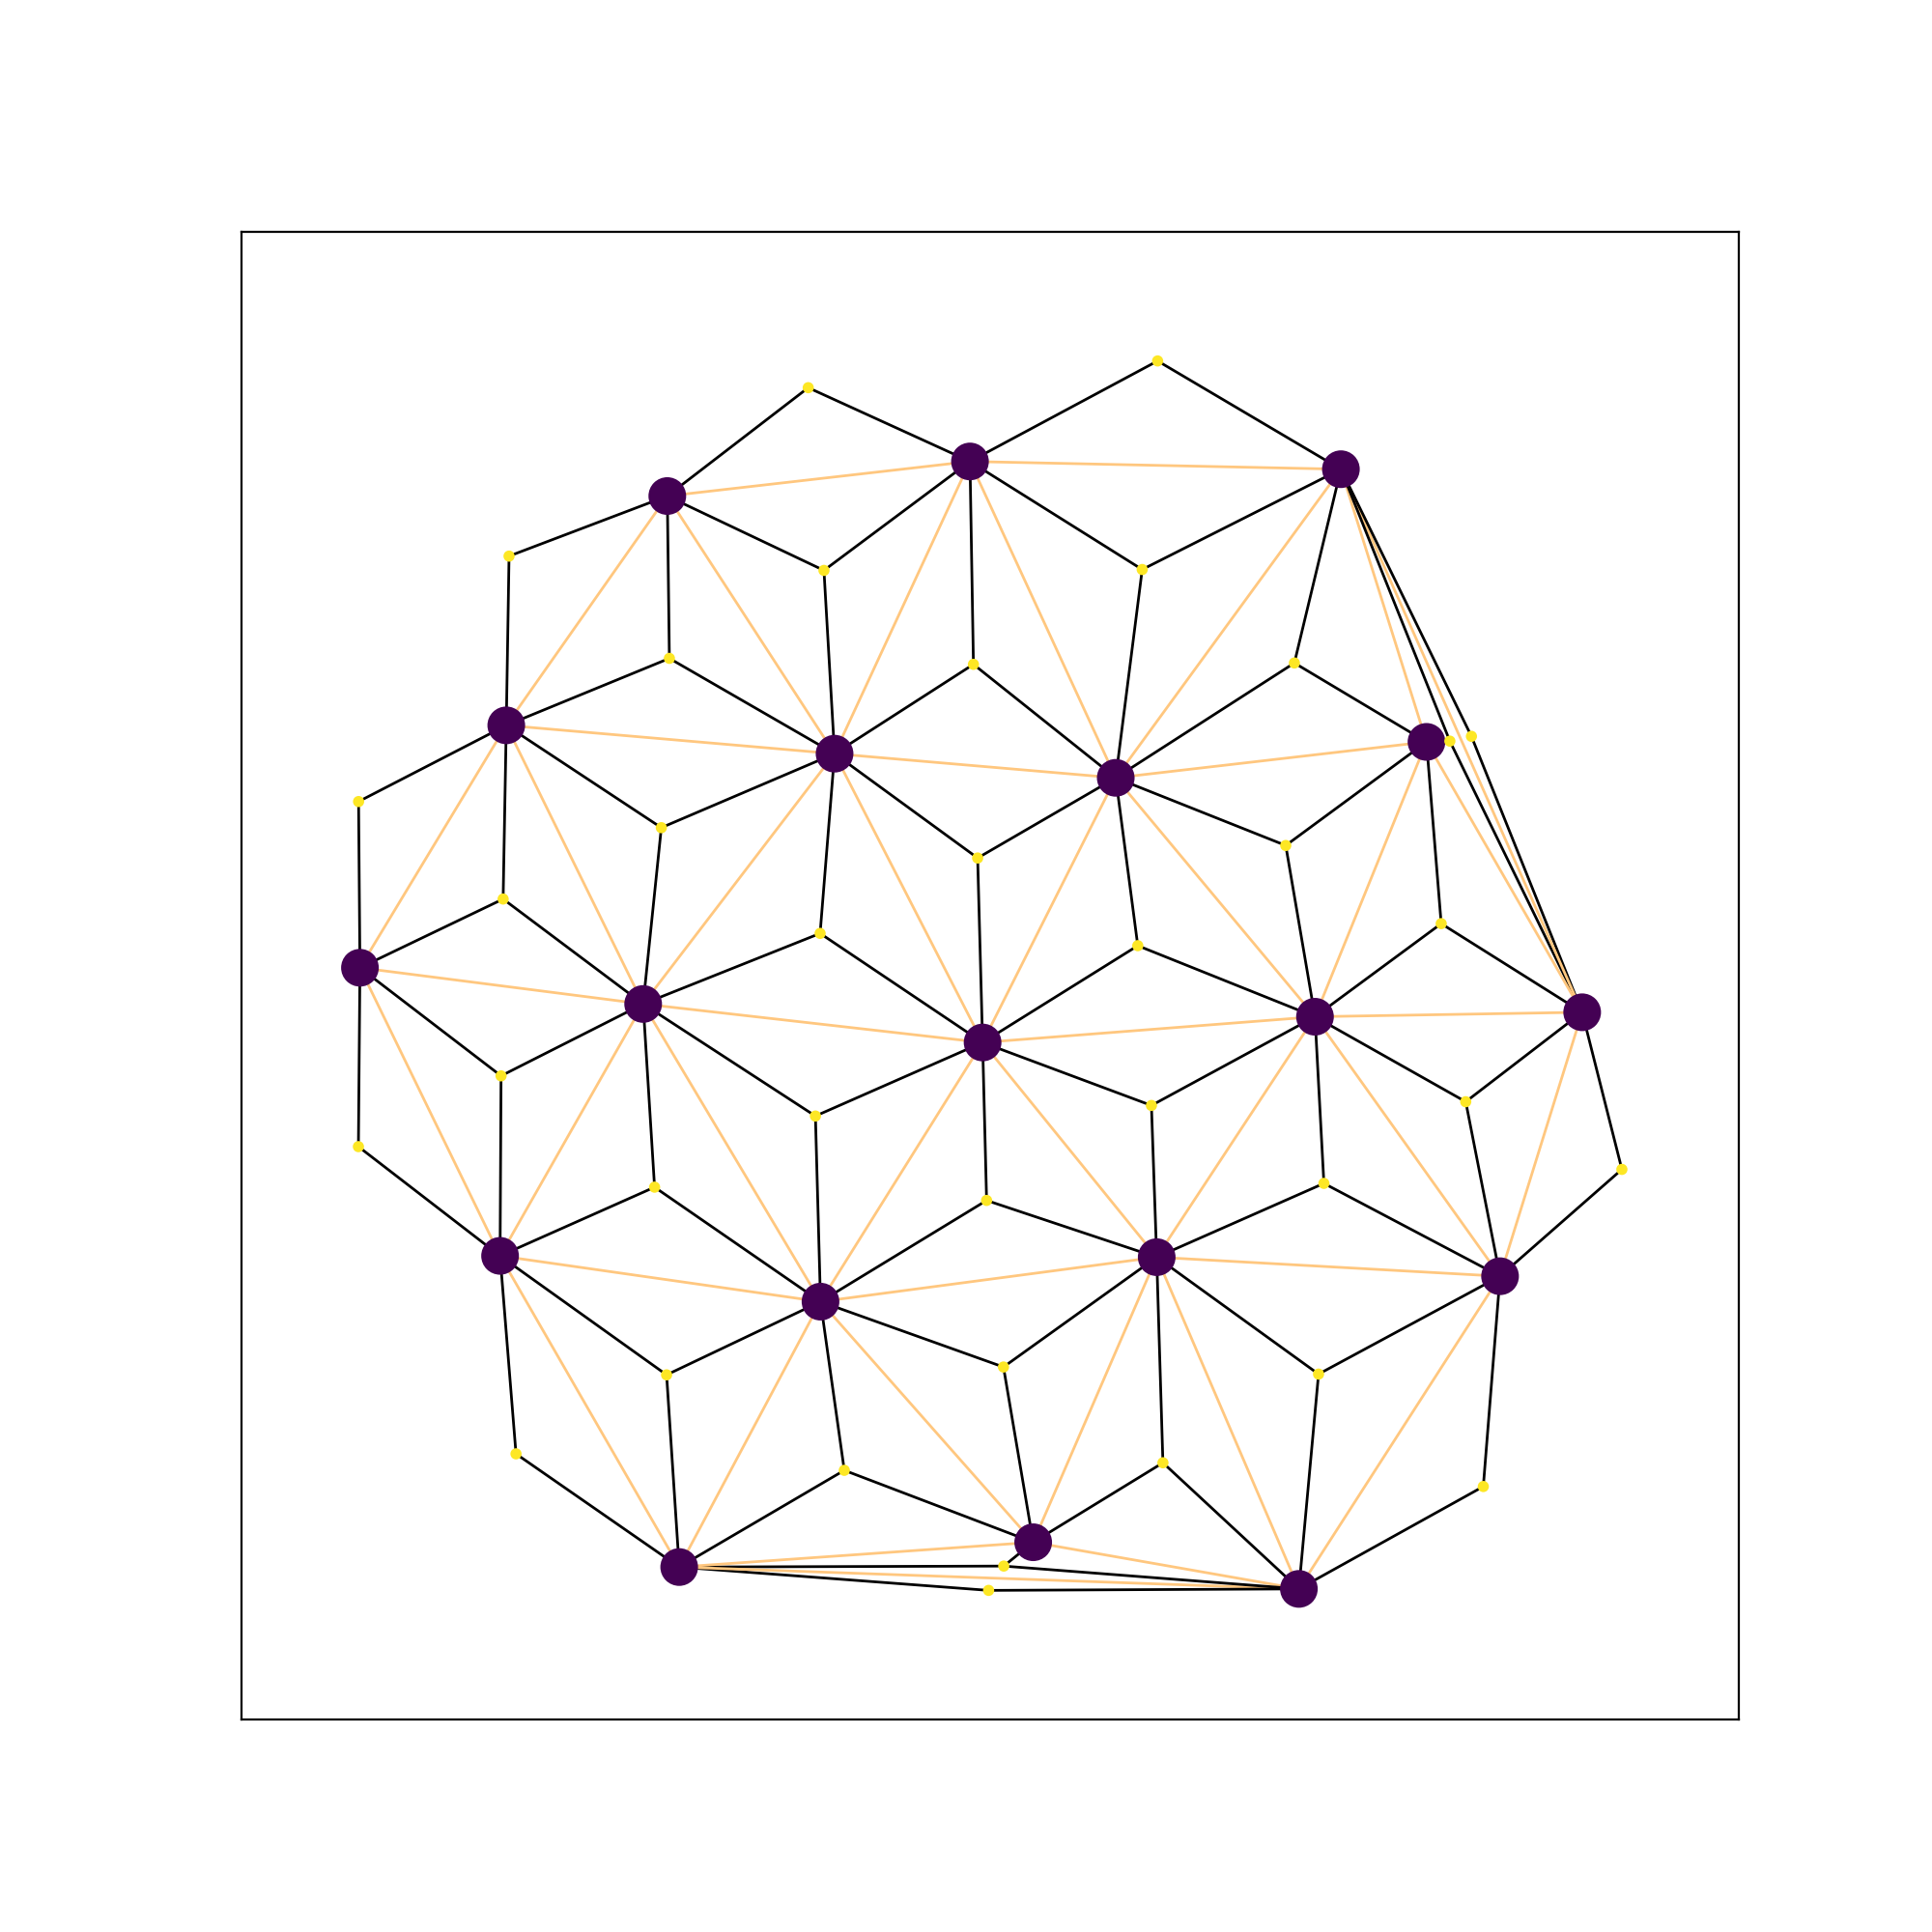
\includegraphics[width=0.5\textwidth]{hexnoise/hexnoise_graph.png}
        \caption{Initial lattice drawn as in Figure \ref{fig:layout_init}.}
        \label{subfig:hexnoise_graph}
    \end{subfigure}
    \begin{subfigure}[b]{\textwidth}
        \centering
        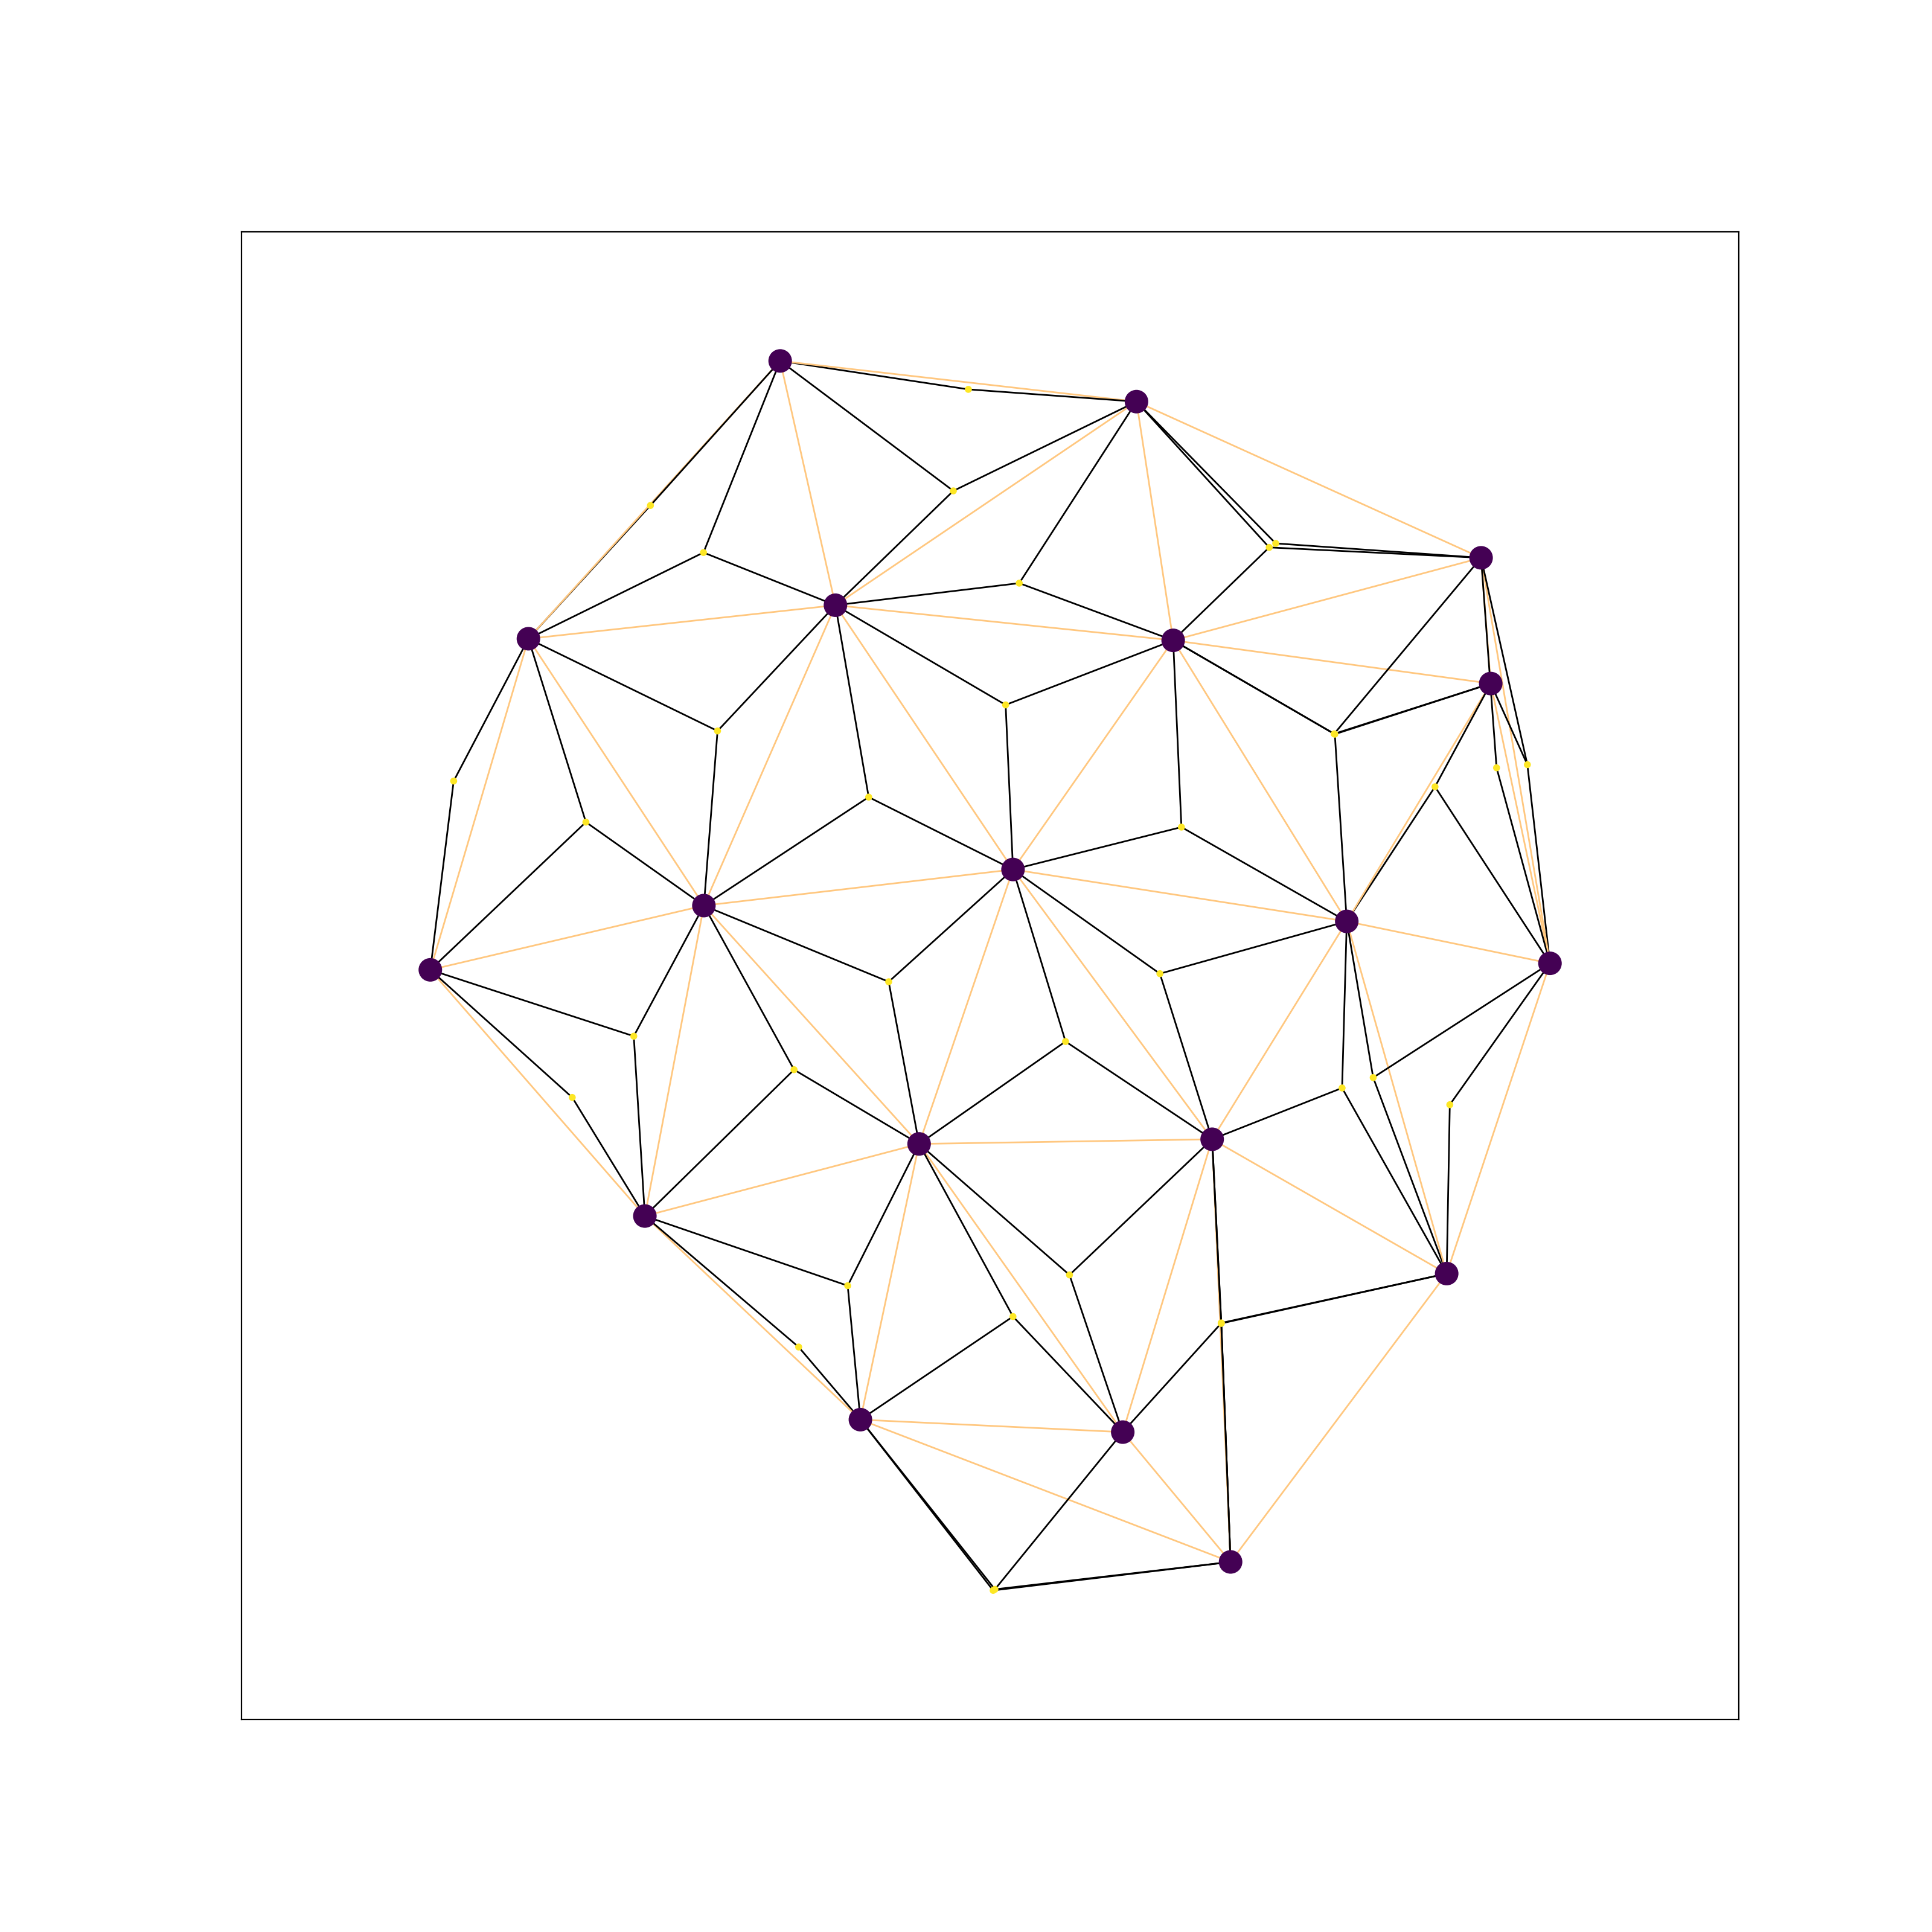
\includegraphics[width=0.3\textwidth]{hexnoise/hexnoise0.8_0.8_1.52_10_graph.png}
        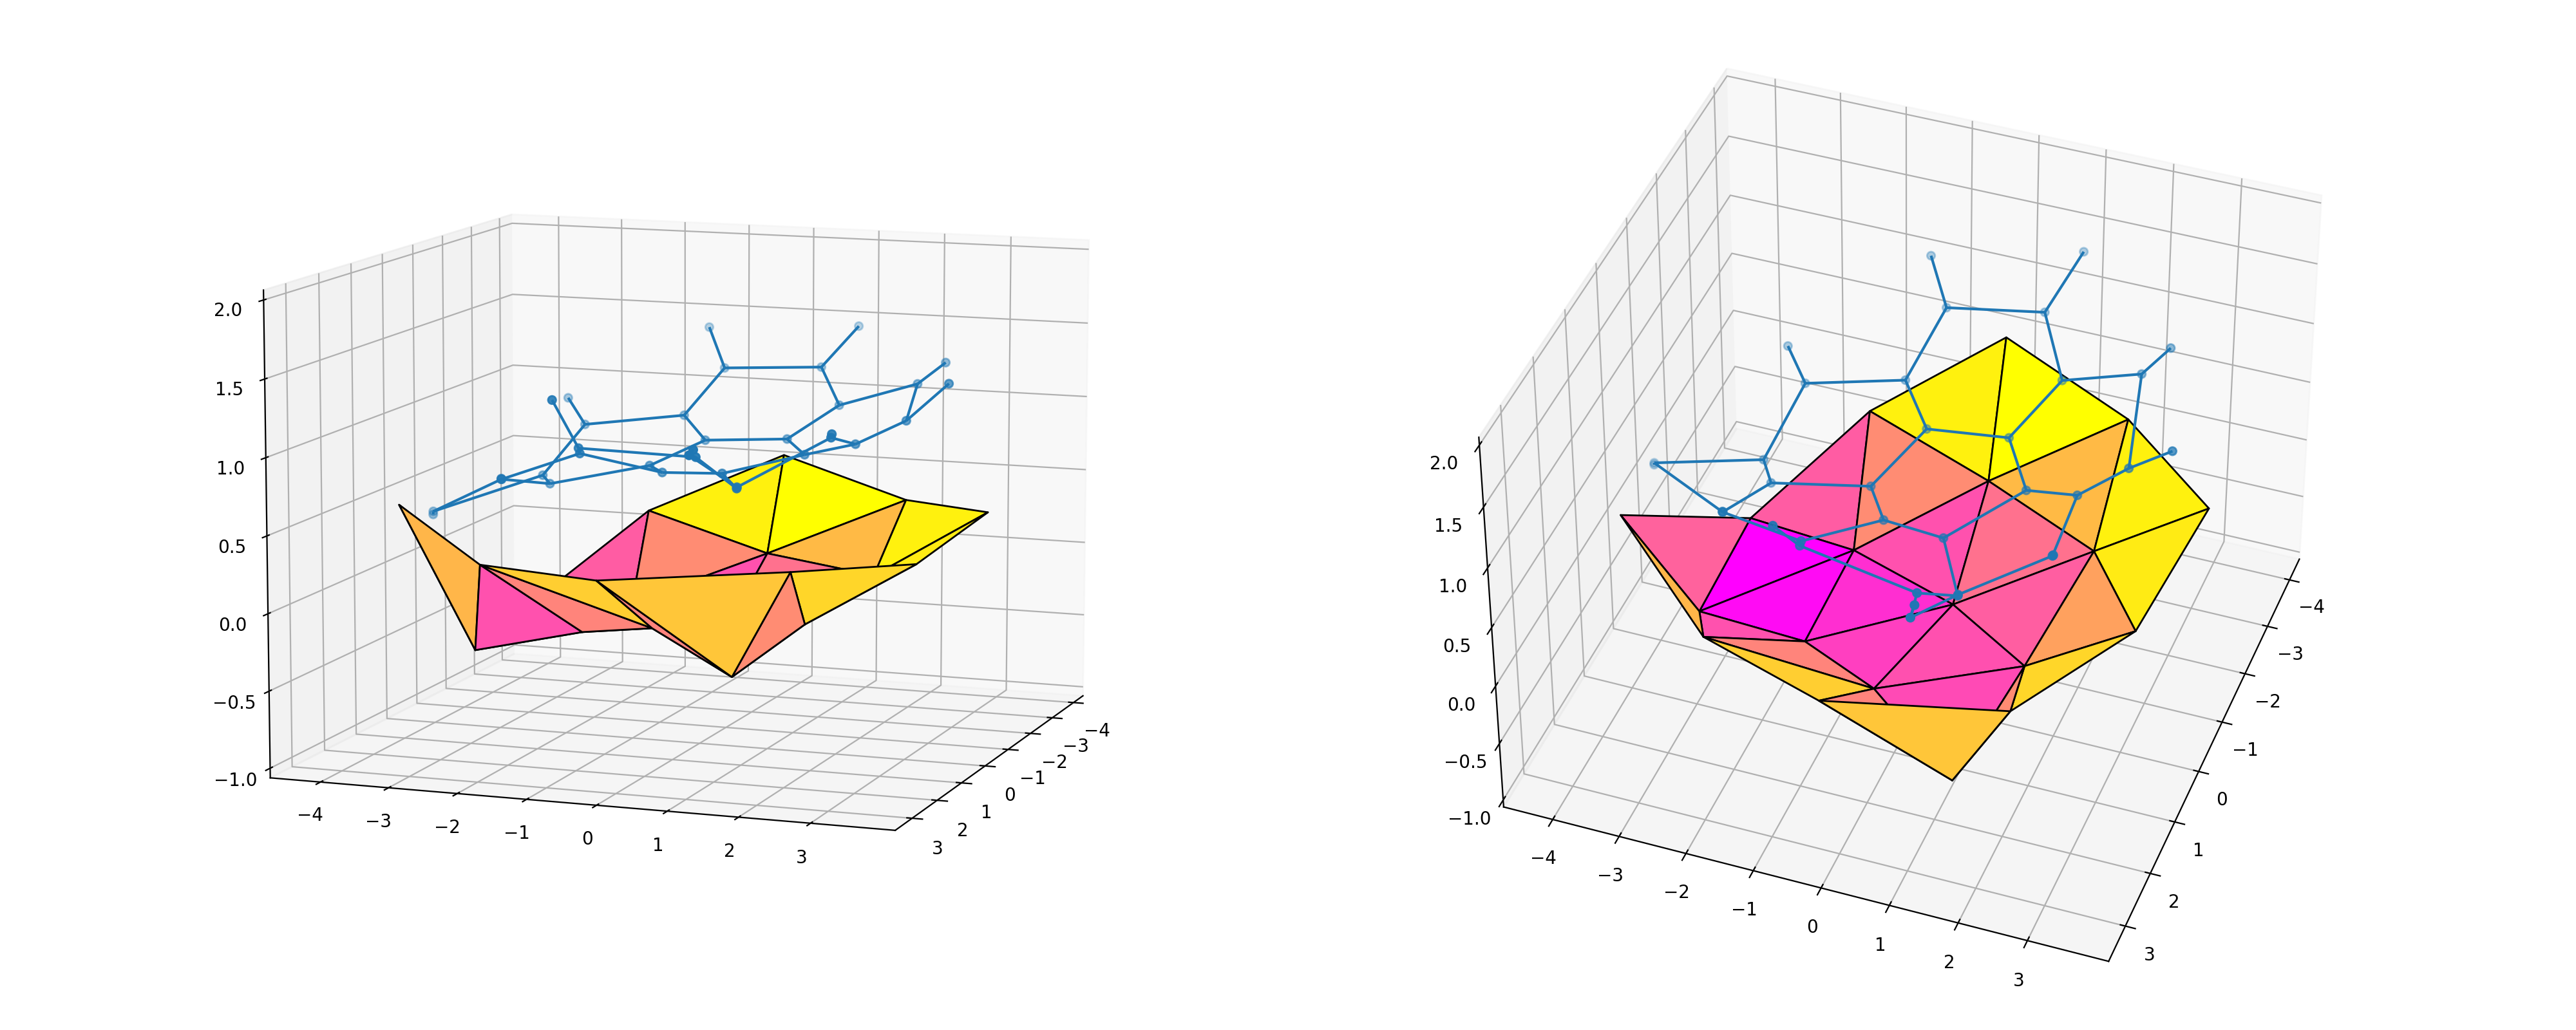
\includegraphics[width=0.69\textwidth]{hexnoise/hexnoise0.8_0.8_1.52_10_plot.png}
        \caption{Sheet shape when $\phi_0=0.8$, $\psi_0=0.8$, $\ell_0=1.52$.}
        \label{subfig:hexnoise_in}
    \end{subfigure}
    \begin{subfigure}[b]{\textwidth}
        \centering
        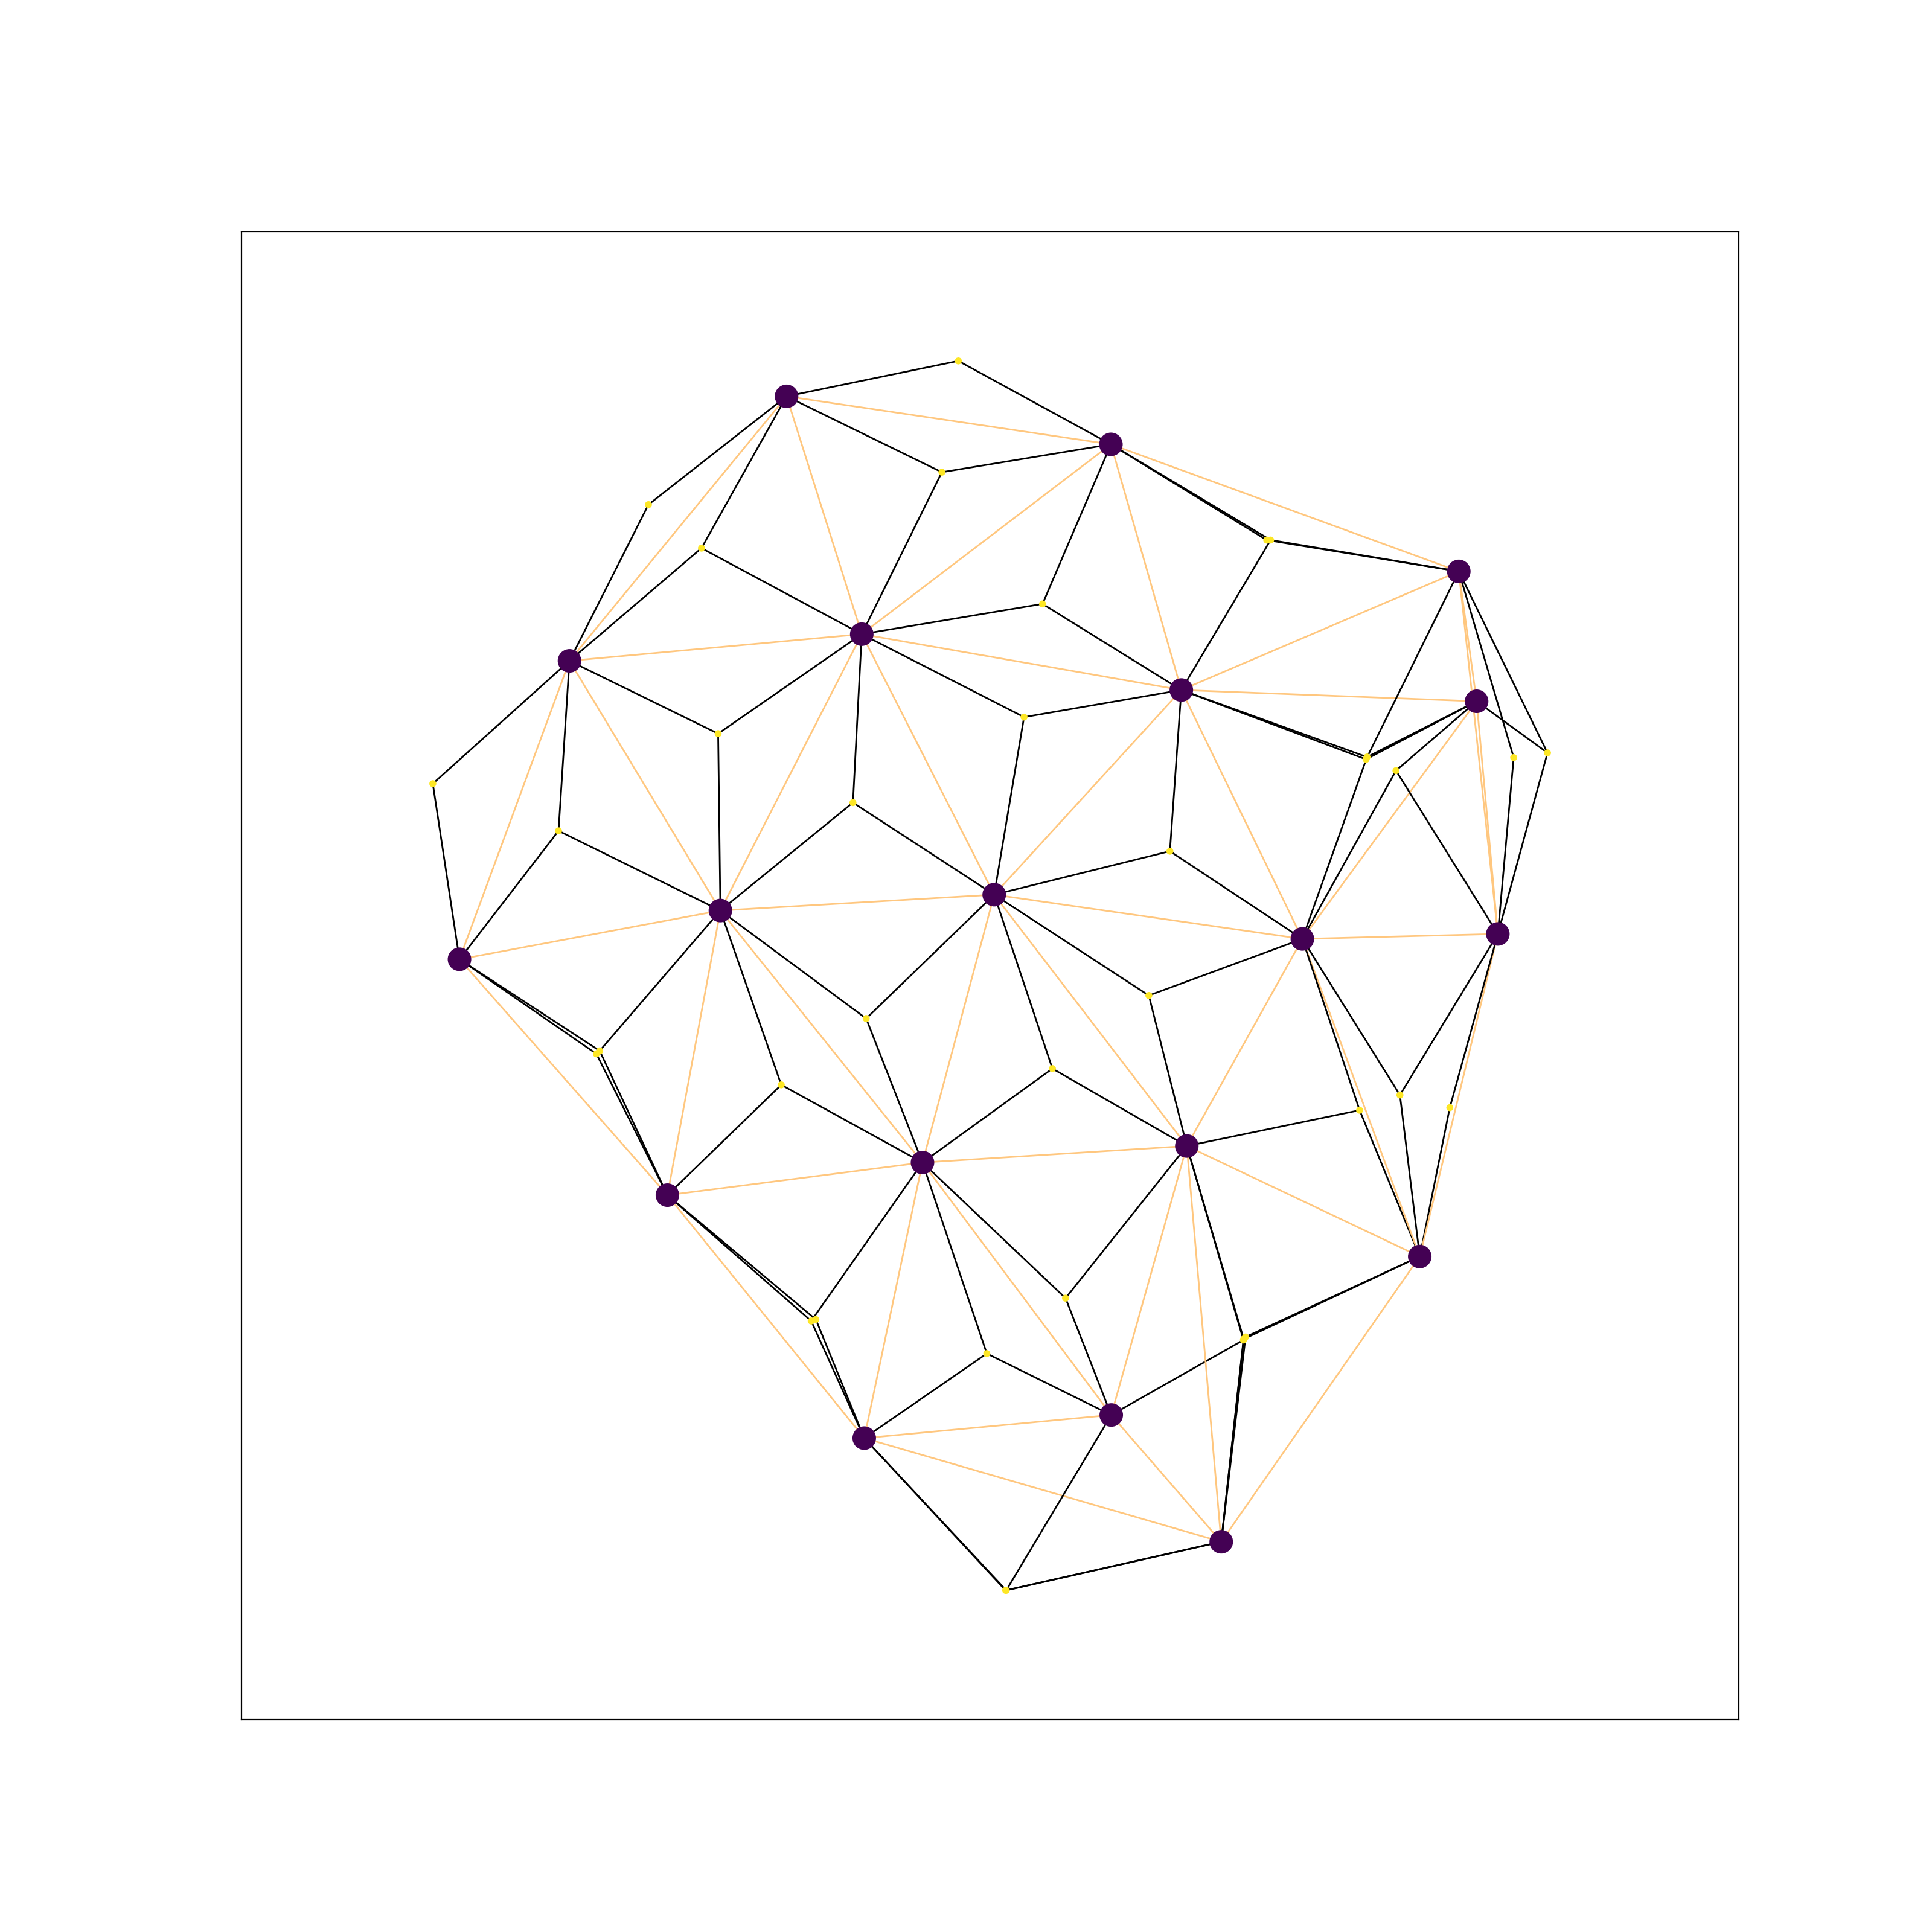
\includegraphics[width=0.3\textwidth]{hexnoise/hexnoise0.95_0.8_1.52_10_graph.png}
        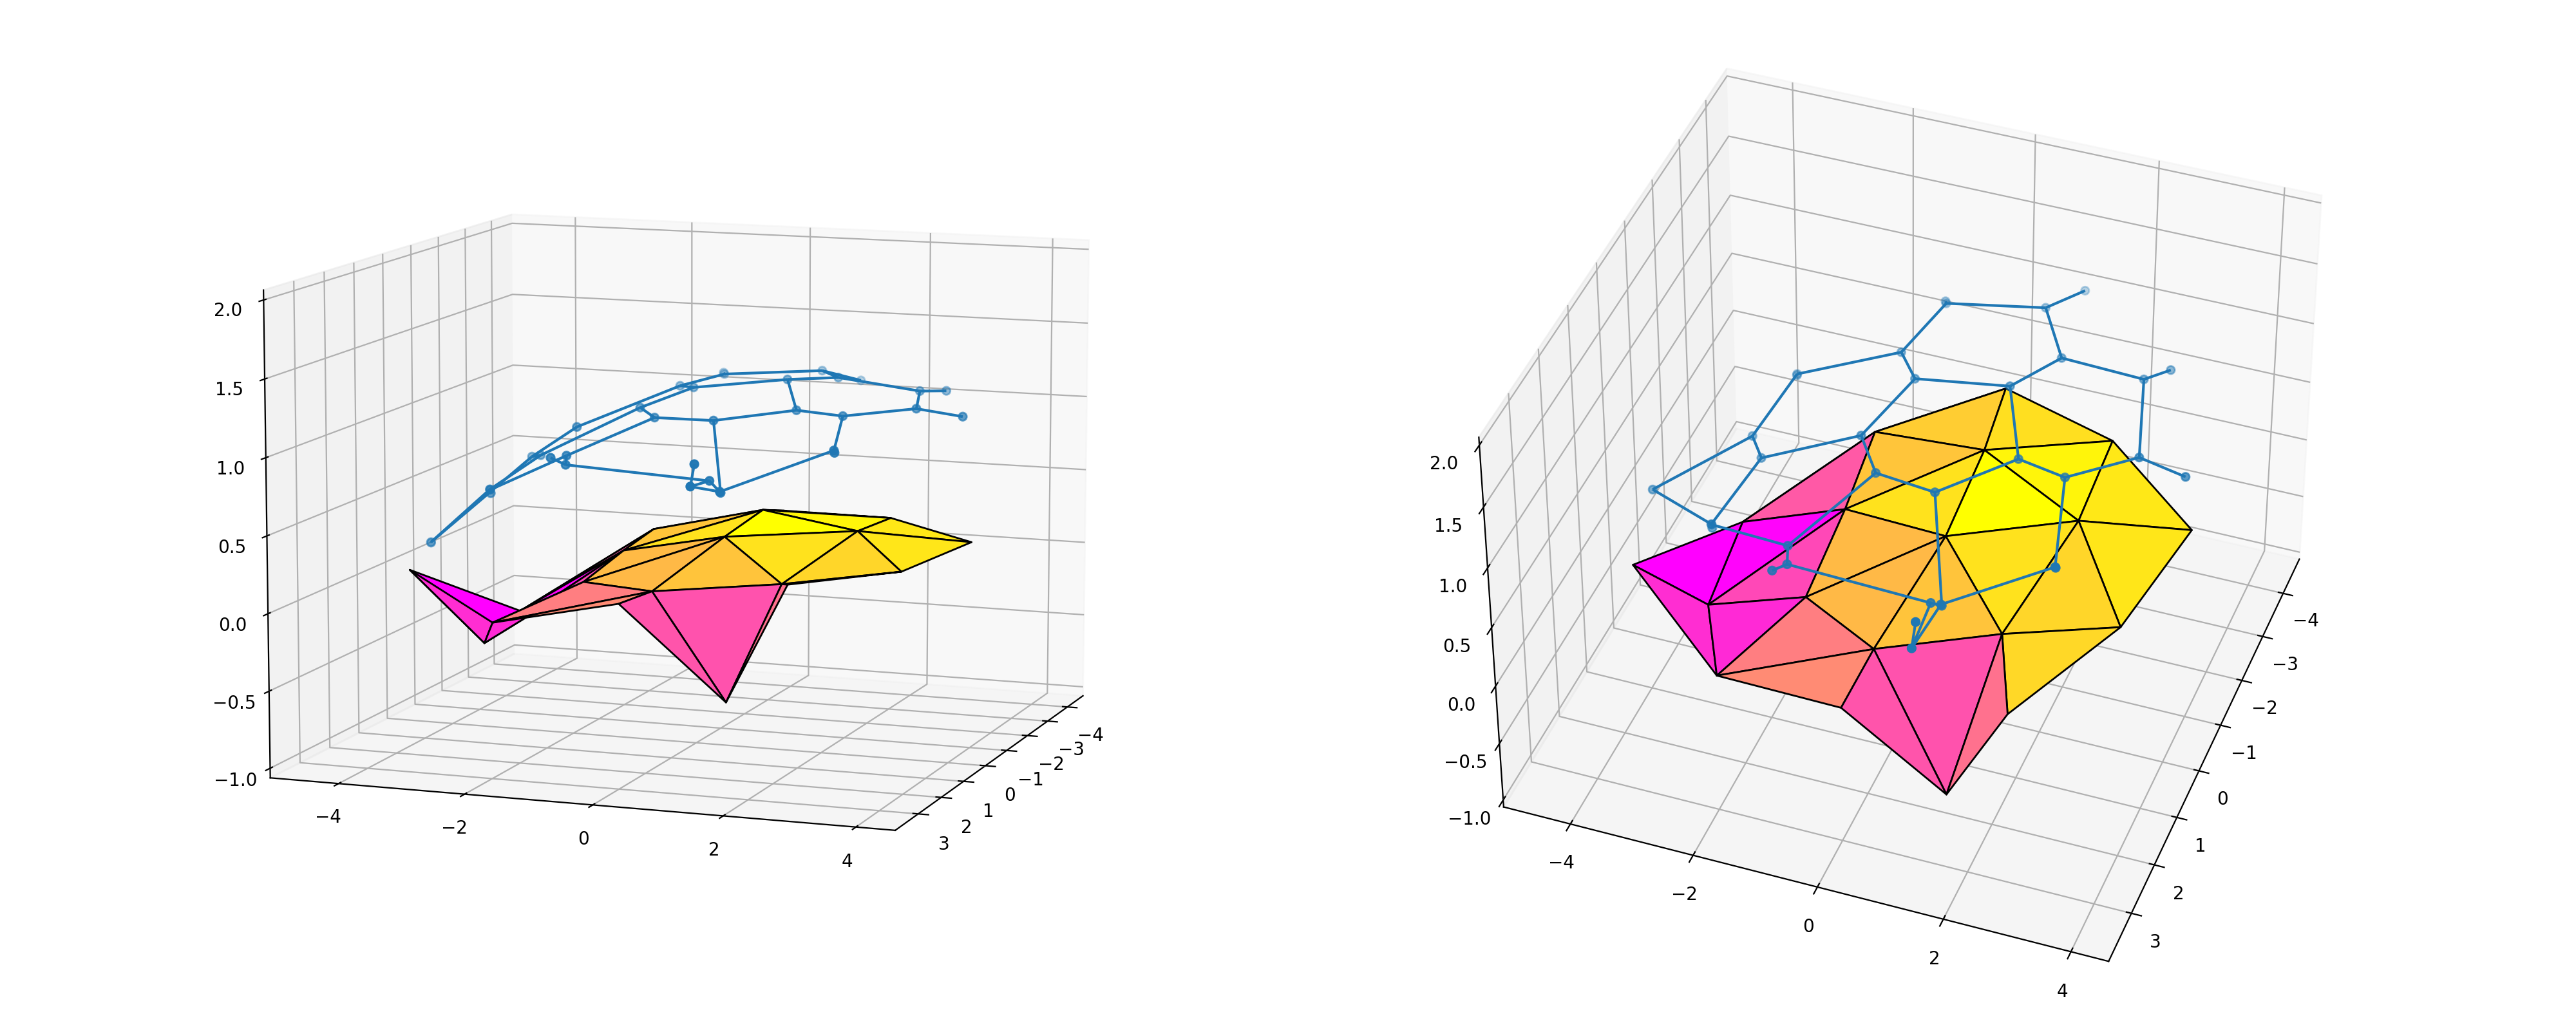
\includegraphics[width=0.69\textwidth]{hexnoise/hexnoise0.95_0.8_1.52_10_plot.png}
        \caption{Sheet shape when $\phi_0=0.95$, $\psi_0=0.8$, $\ell_0=1.52$.}
        \label{subfig:hexnoise_out}
    \end{subfigure}
    \caption{Cell sheet geometry with noise added to the initial lattice. The graph topology is affected at the sheet boundary (subfigure \ref{subfig:hexnoise_graph}) from the Voronoi tesselation. This minor change has substantial effects on the sheet geometry (subfigures \ref{subfig:hexnoise_in}, \ref{subfig:hexnoise_out}).}
    \label{fig:hexnoise}
\end{figure}

\subsubsection{Interior cell topology}

We can also add or merge nodes in a regular lattice (Figure \ref{fig:layout_init}) to introduce nodes with irregular degree. There are more complex ways of making different graph topologies (like Lloyd's initial icosphere) but I don't have curved initial conditions or more complicated lattices implemented yet. 

Figure \ref{fig:kink} shows a sheet with cell of degree 7 (7 bordering cells) and \ref{fig:bump} shows a sheet with two neighboring cells of degree 5. 

\begin{figure}[htbp]
    \centering
    \begin{subfigure}[b]{\textwidth}
        \centering
        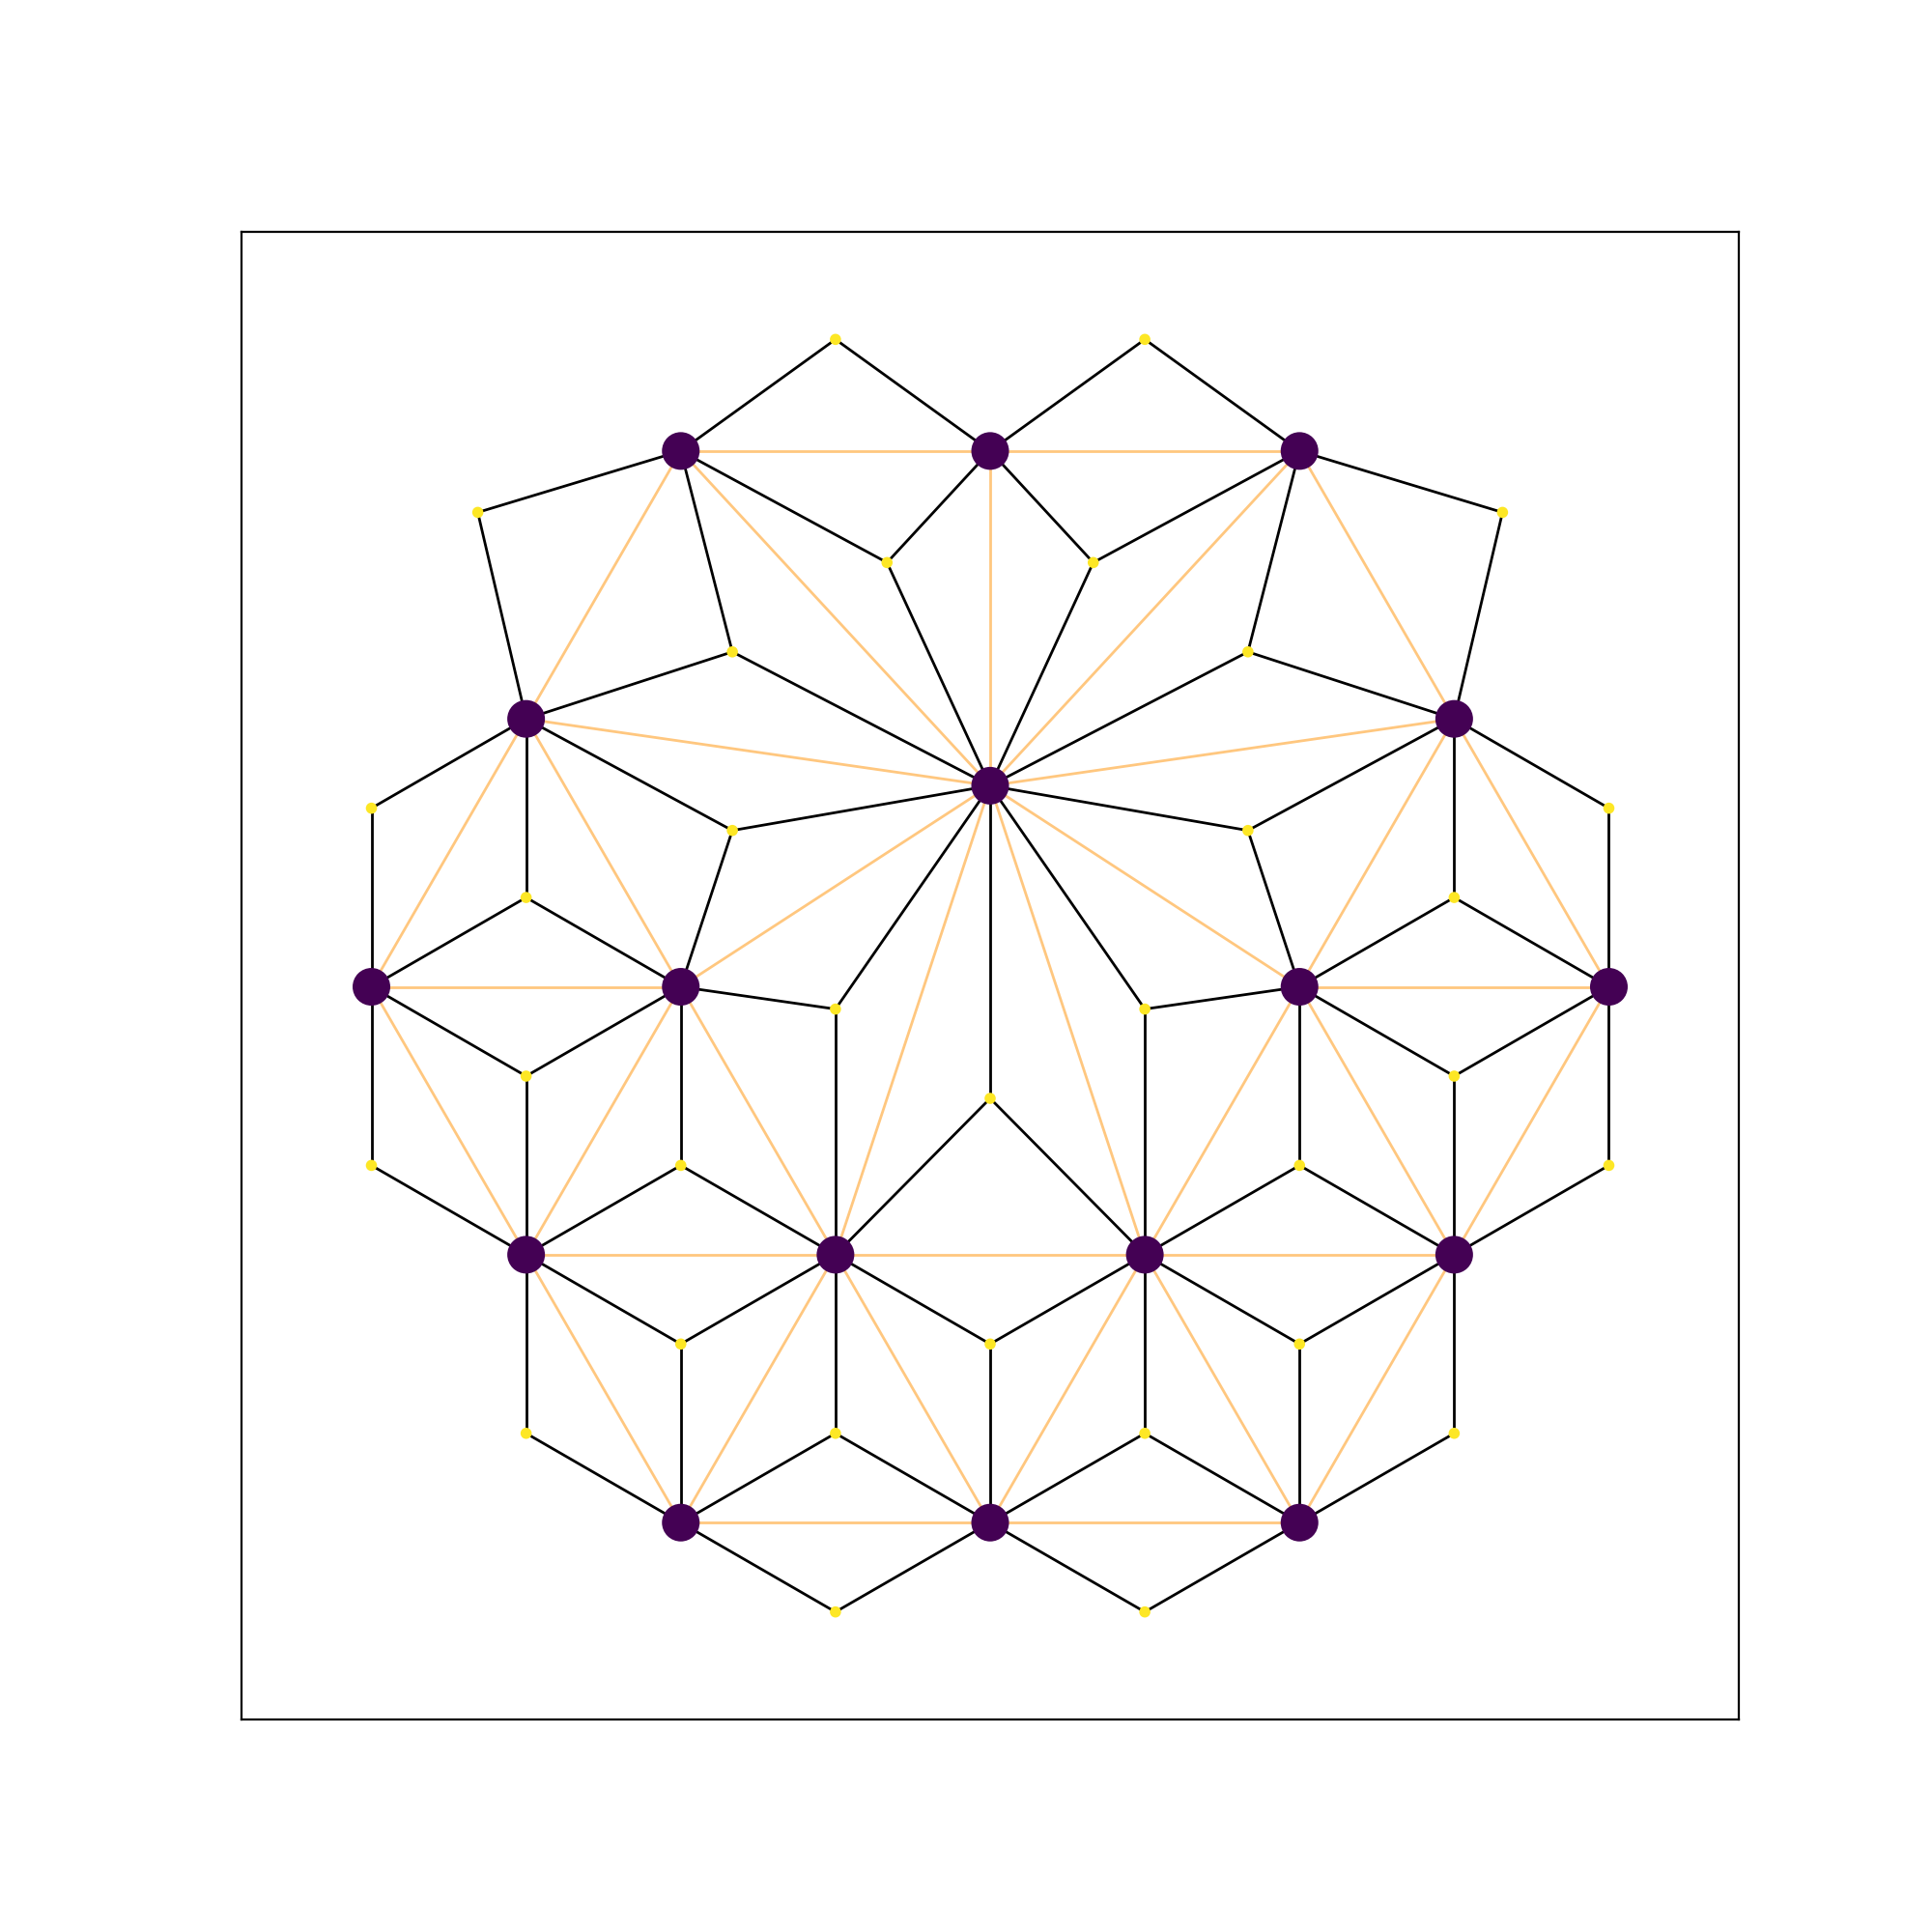
\includegraphics[width=0.5\textwidth]{kink/kink_graph.png}
        \caption{Initial lattice drawn as in Figure \ref{fig:layout_init}.}
        \label{subfig:kink_graph}
    \end{subfigure}
    \begin{subfigure}[b]{\textwidth}
        \centering
        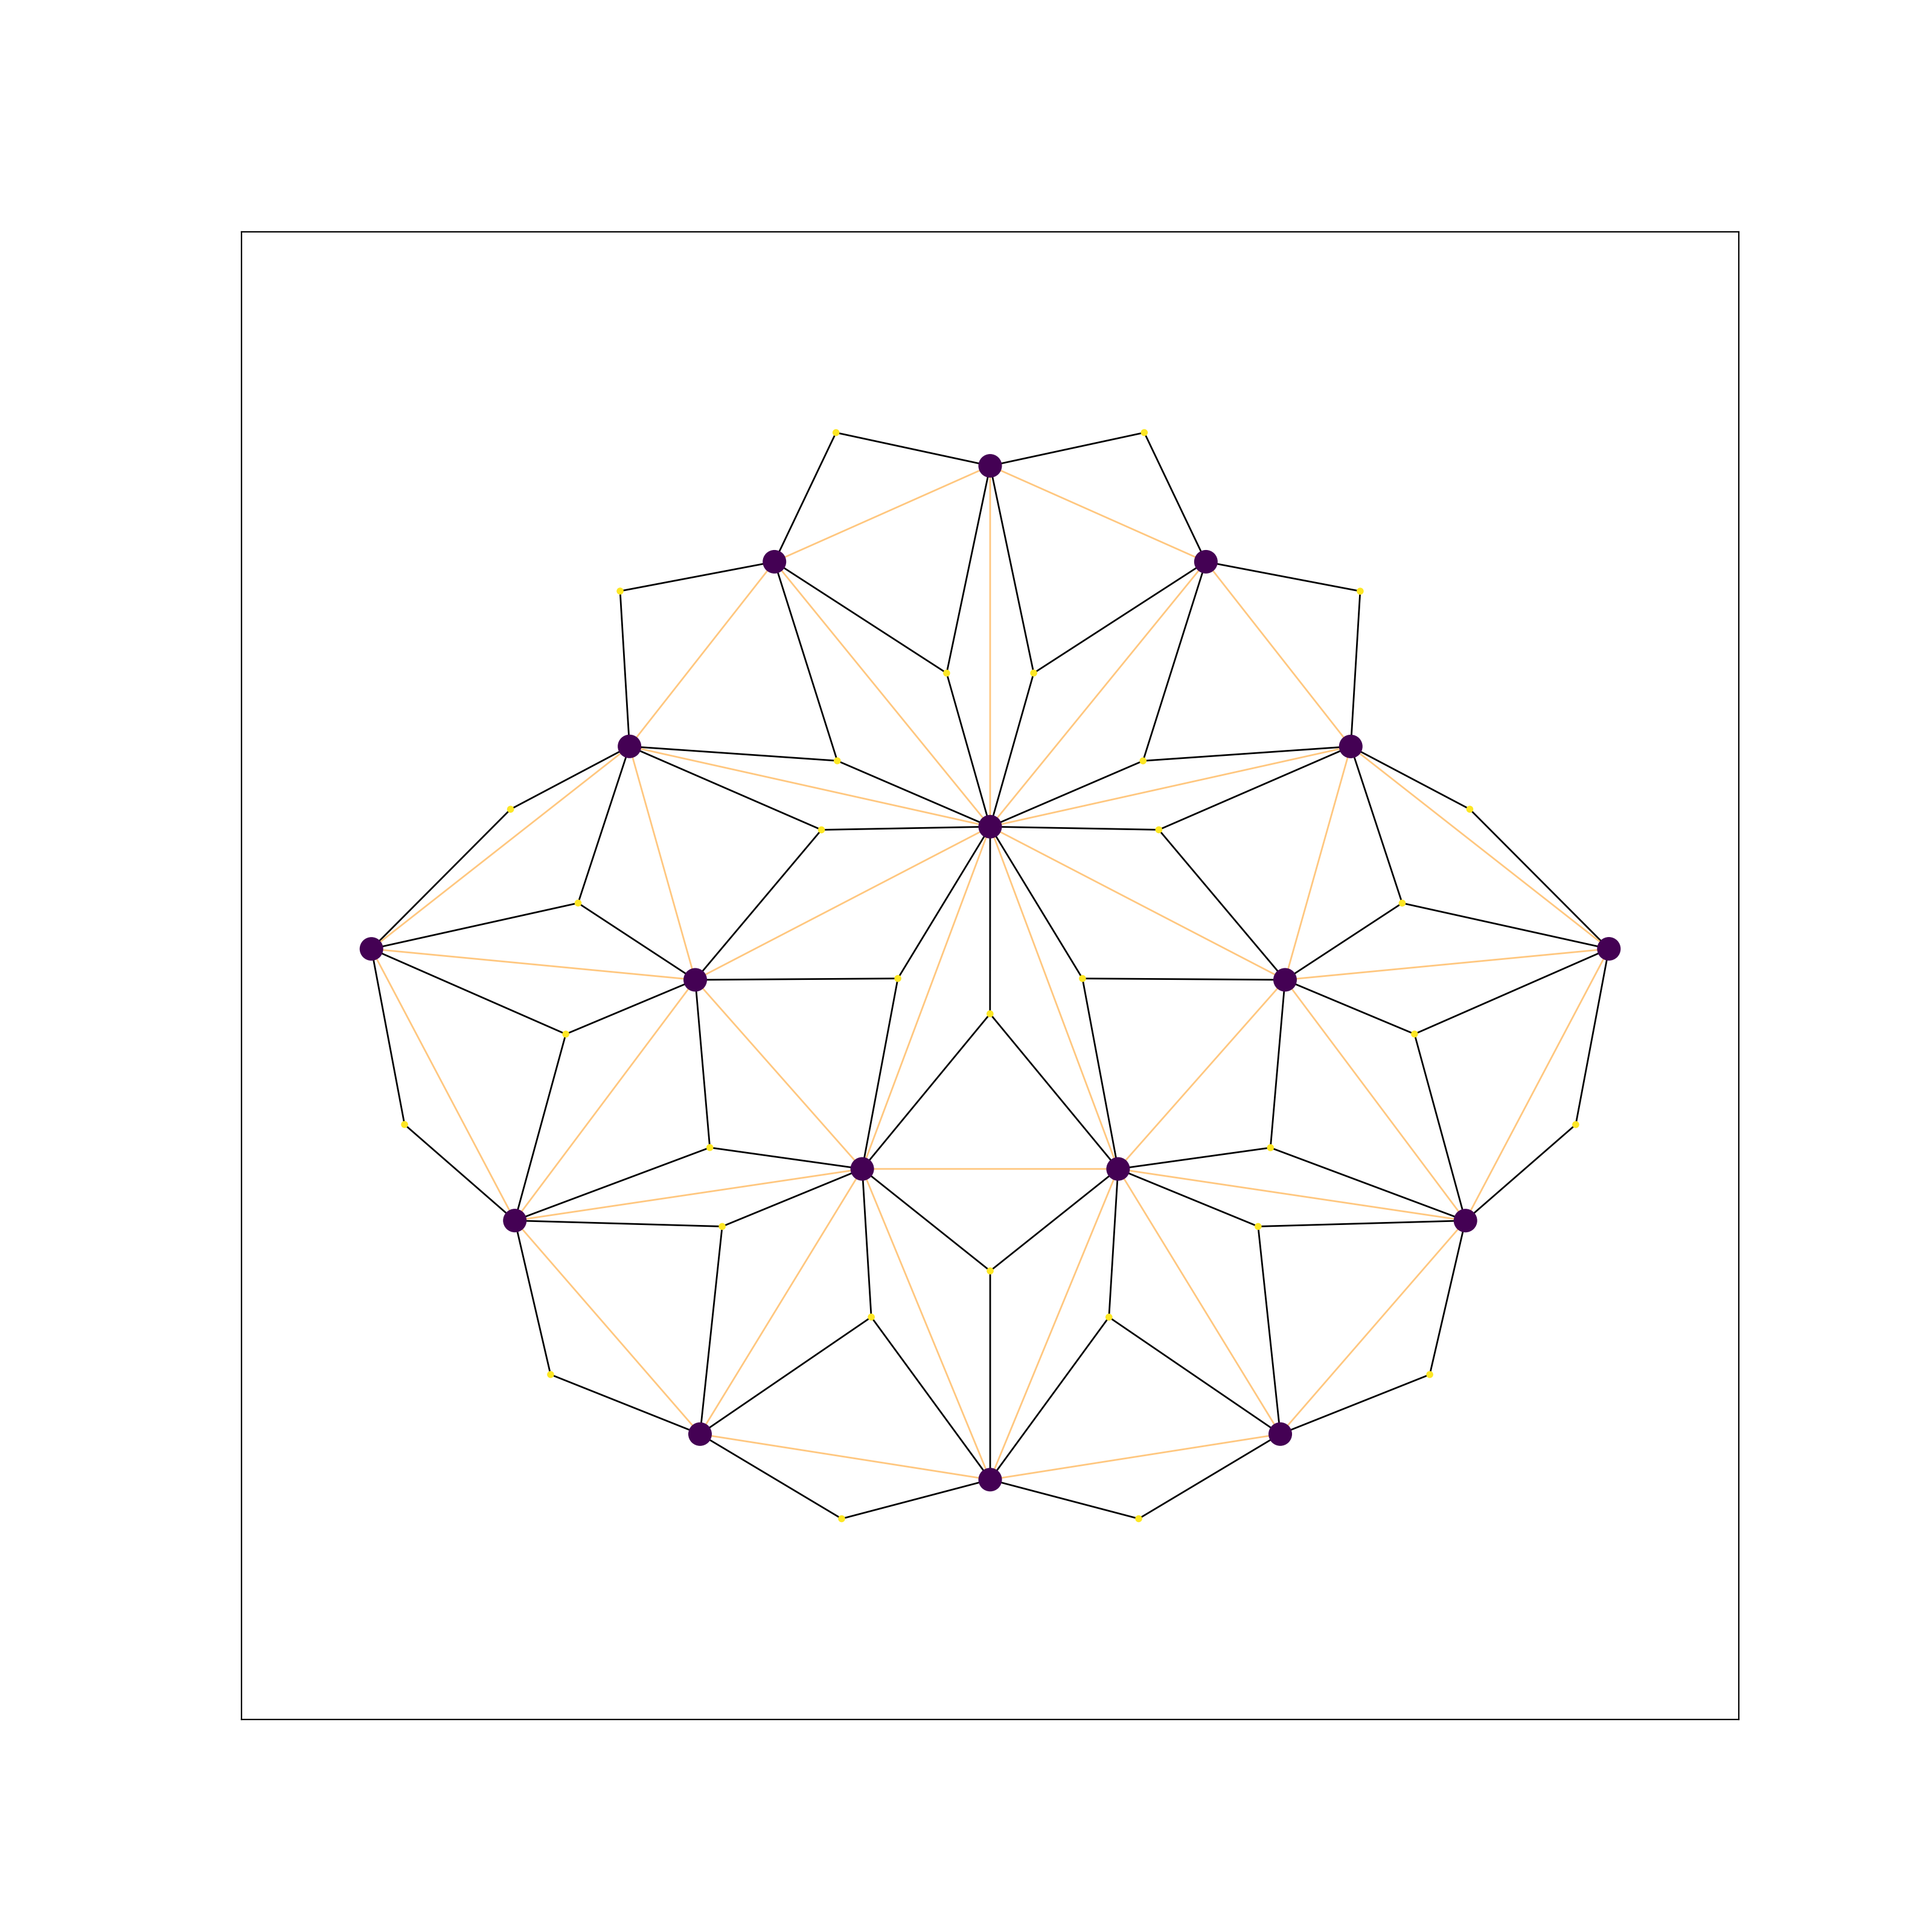
\includegraphics[width=0.3\textwidth]{kink/kink0.8_0.8_1.52_10_graph.png}
        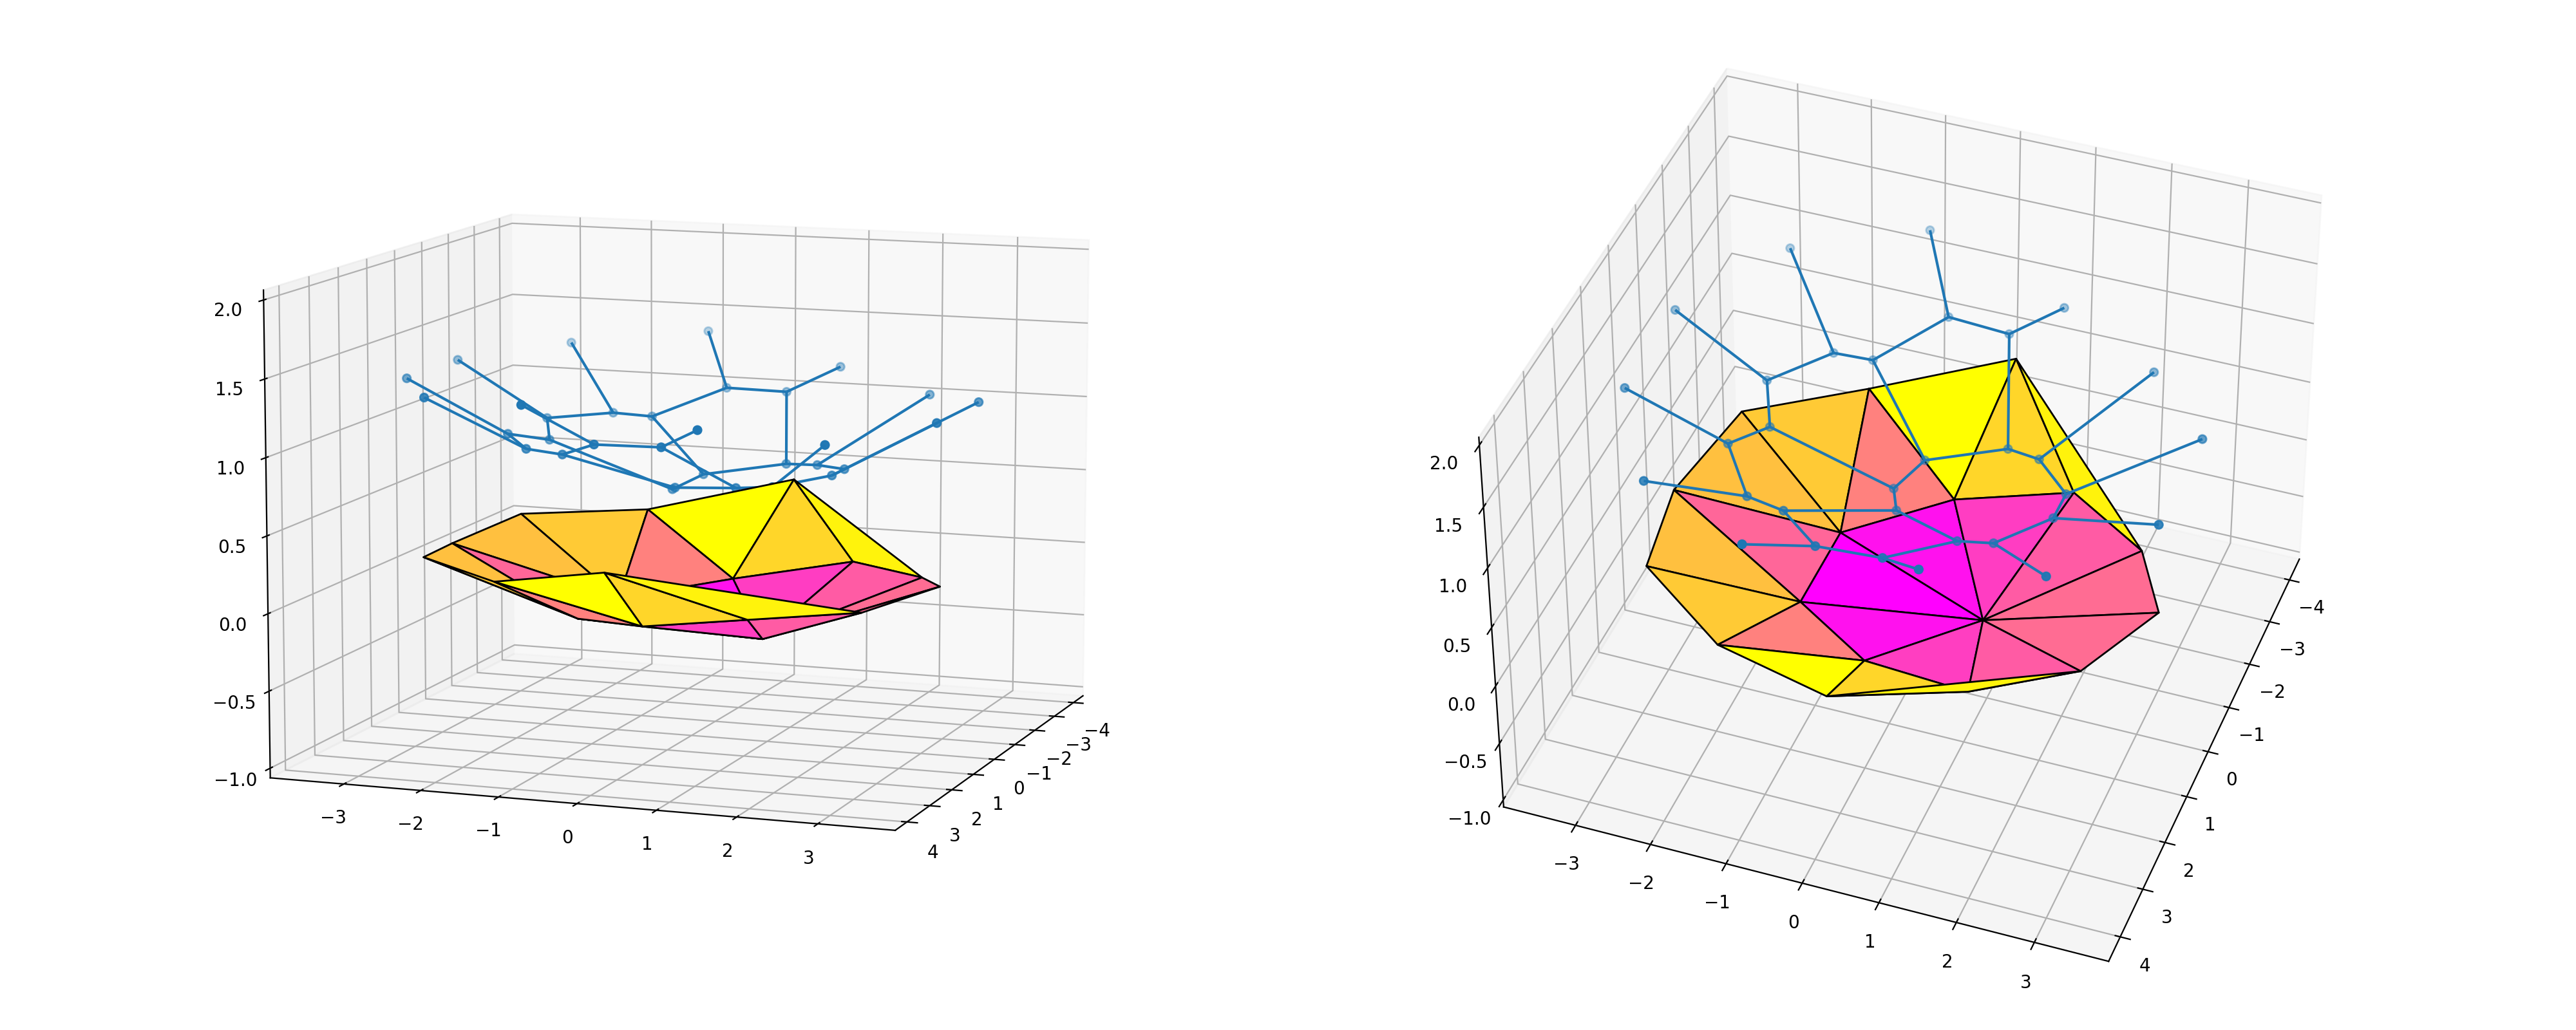
\includegraphics[width=0.69\textwidth]{kink/kink0.8_0.8_1.52_10_plot.png}
        \caption{Sheet shape when $\phi_0=0.8$, $\psi_0=0.8$, $\ell_0=1.52$.}
        \label{subfig:kink_in}
    \end{subfigure}
    \begin{subfigure}[b]{\textwidth}
        \centering
        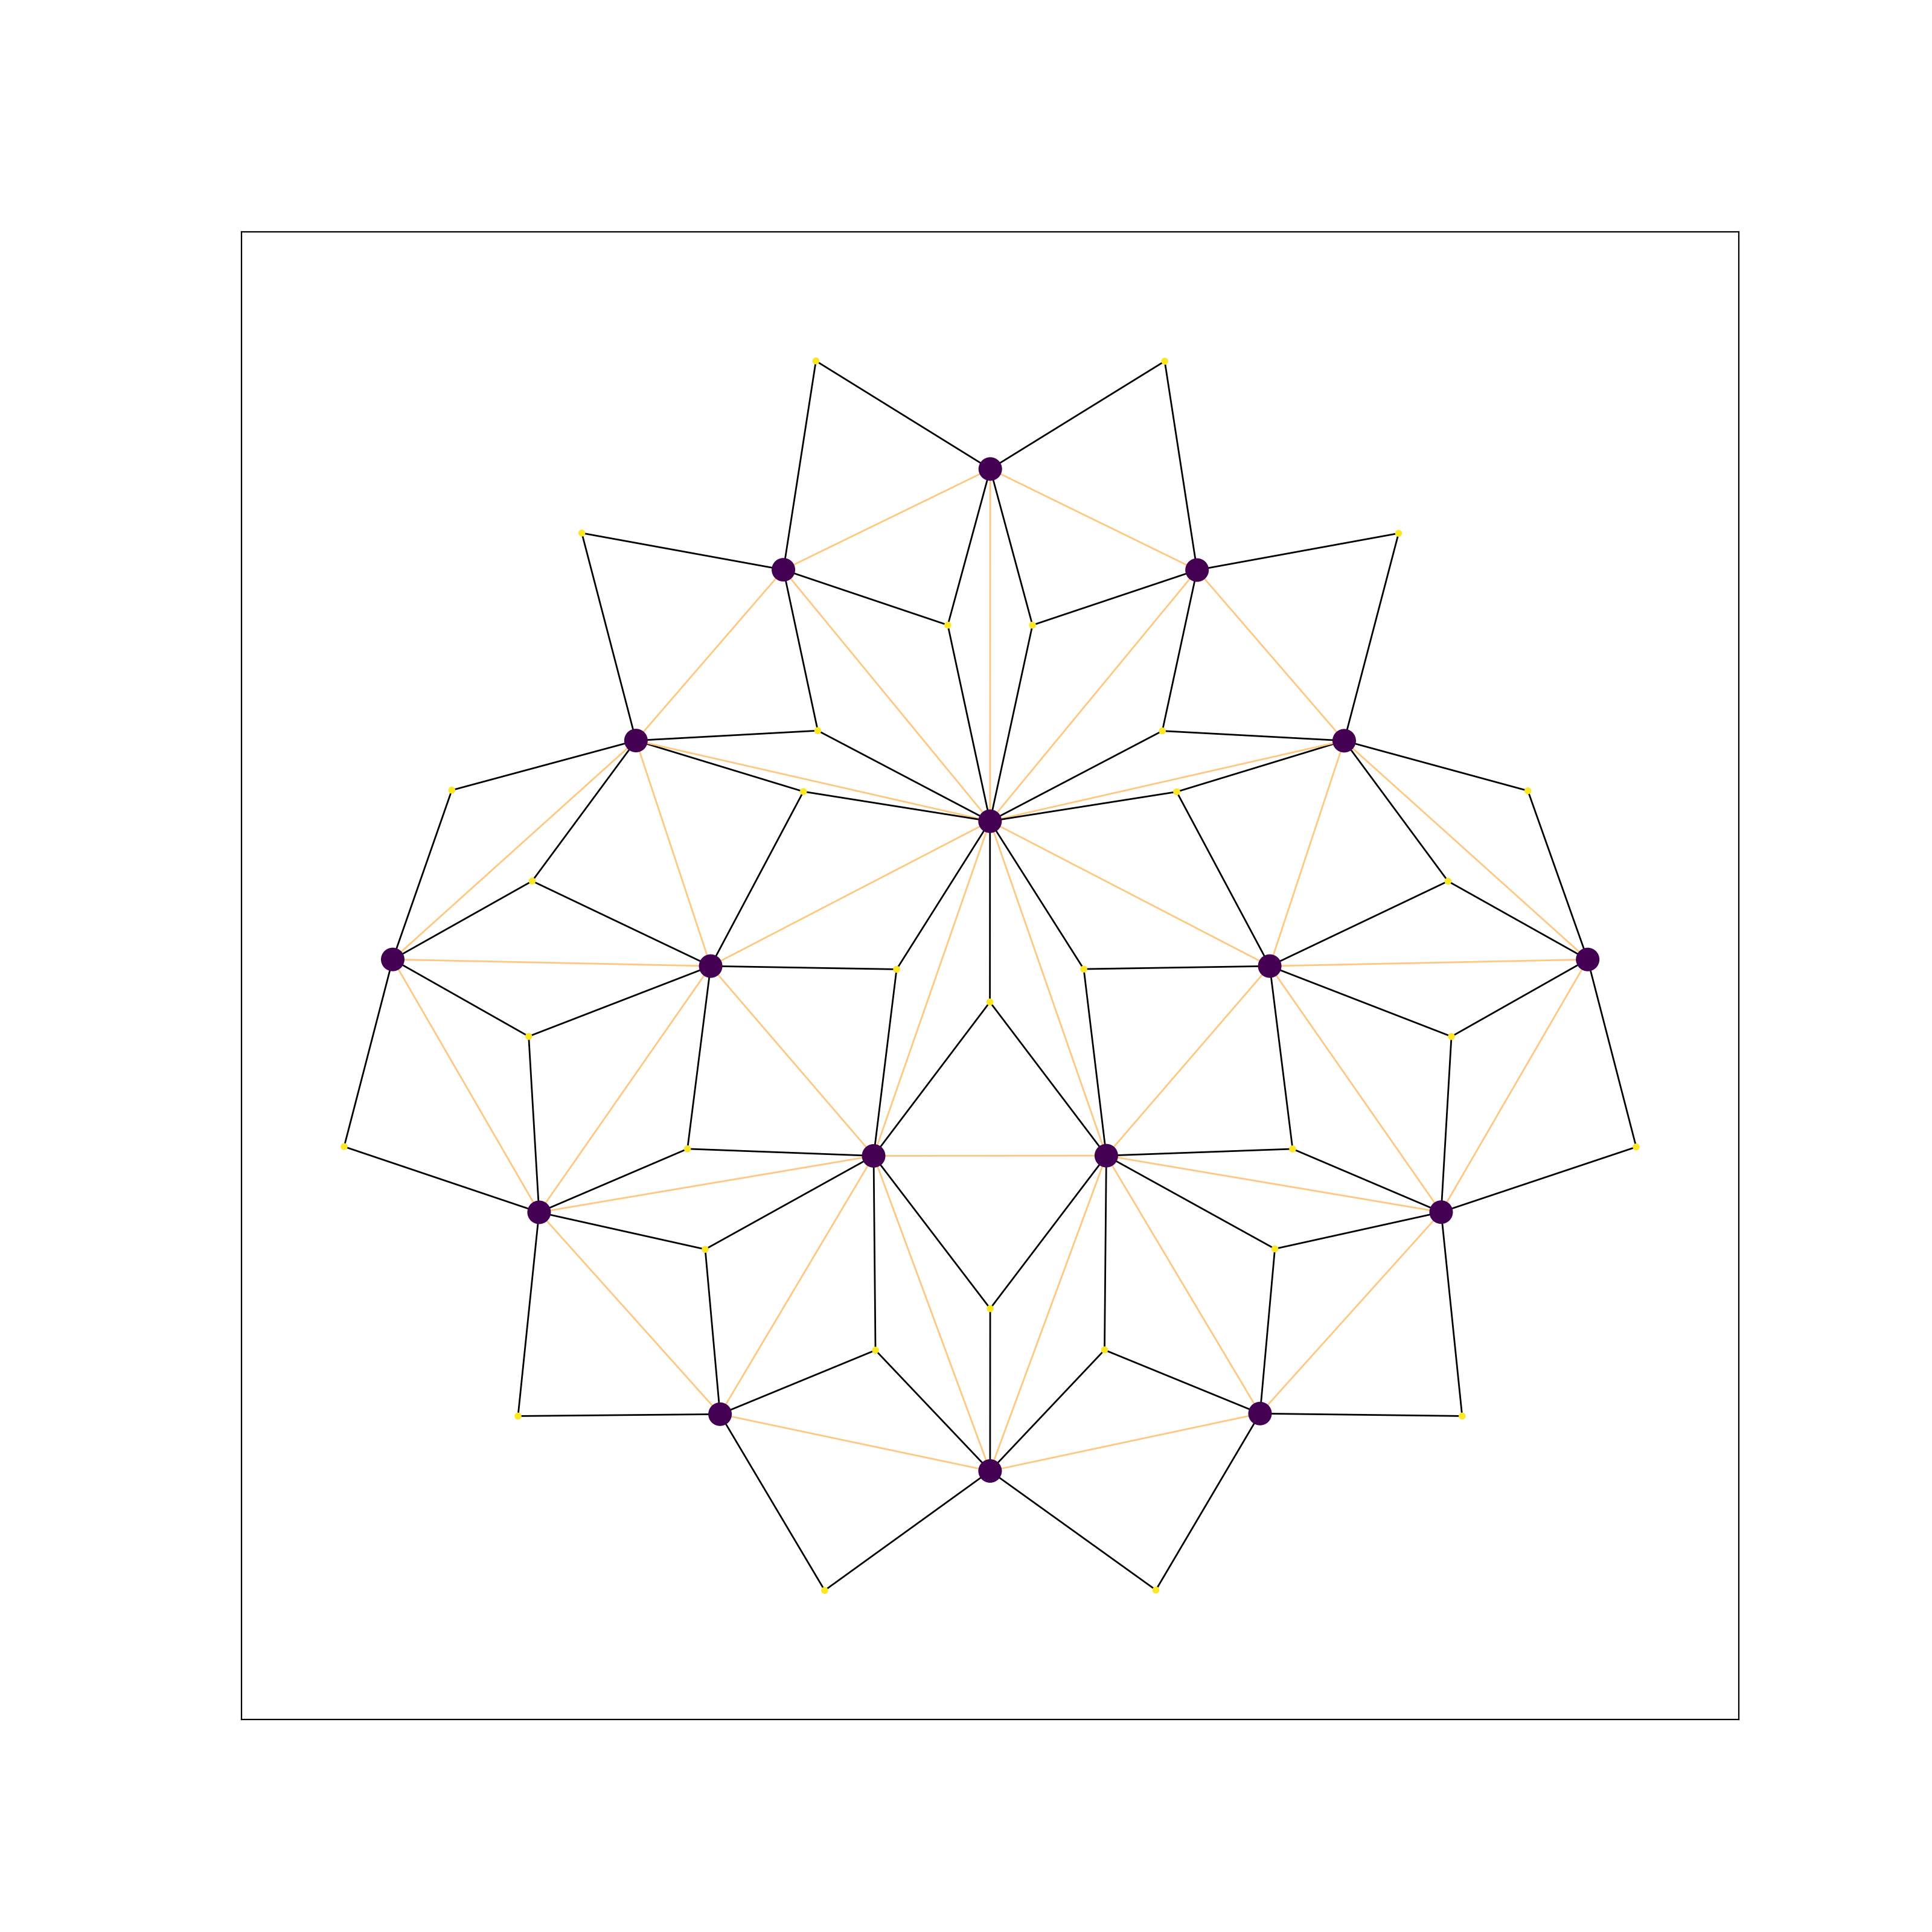
\includegraphics[width=0.3\textwidth]{kink/kink0.95_0.8_1.52_10_graph.png}
        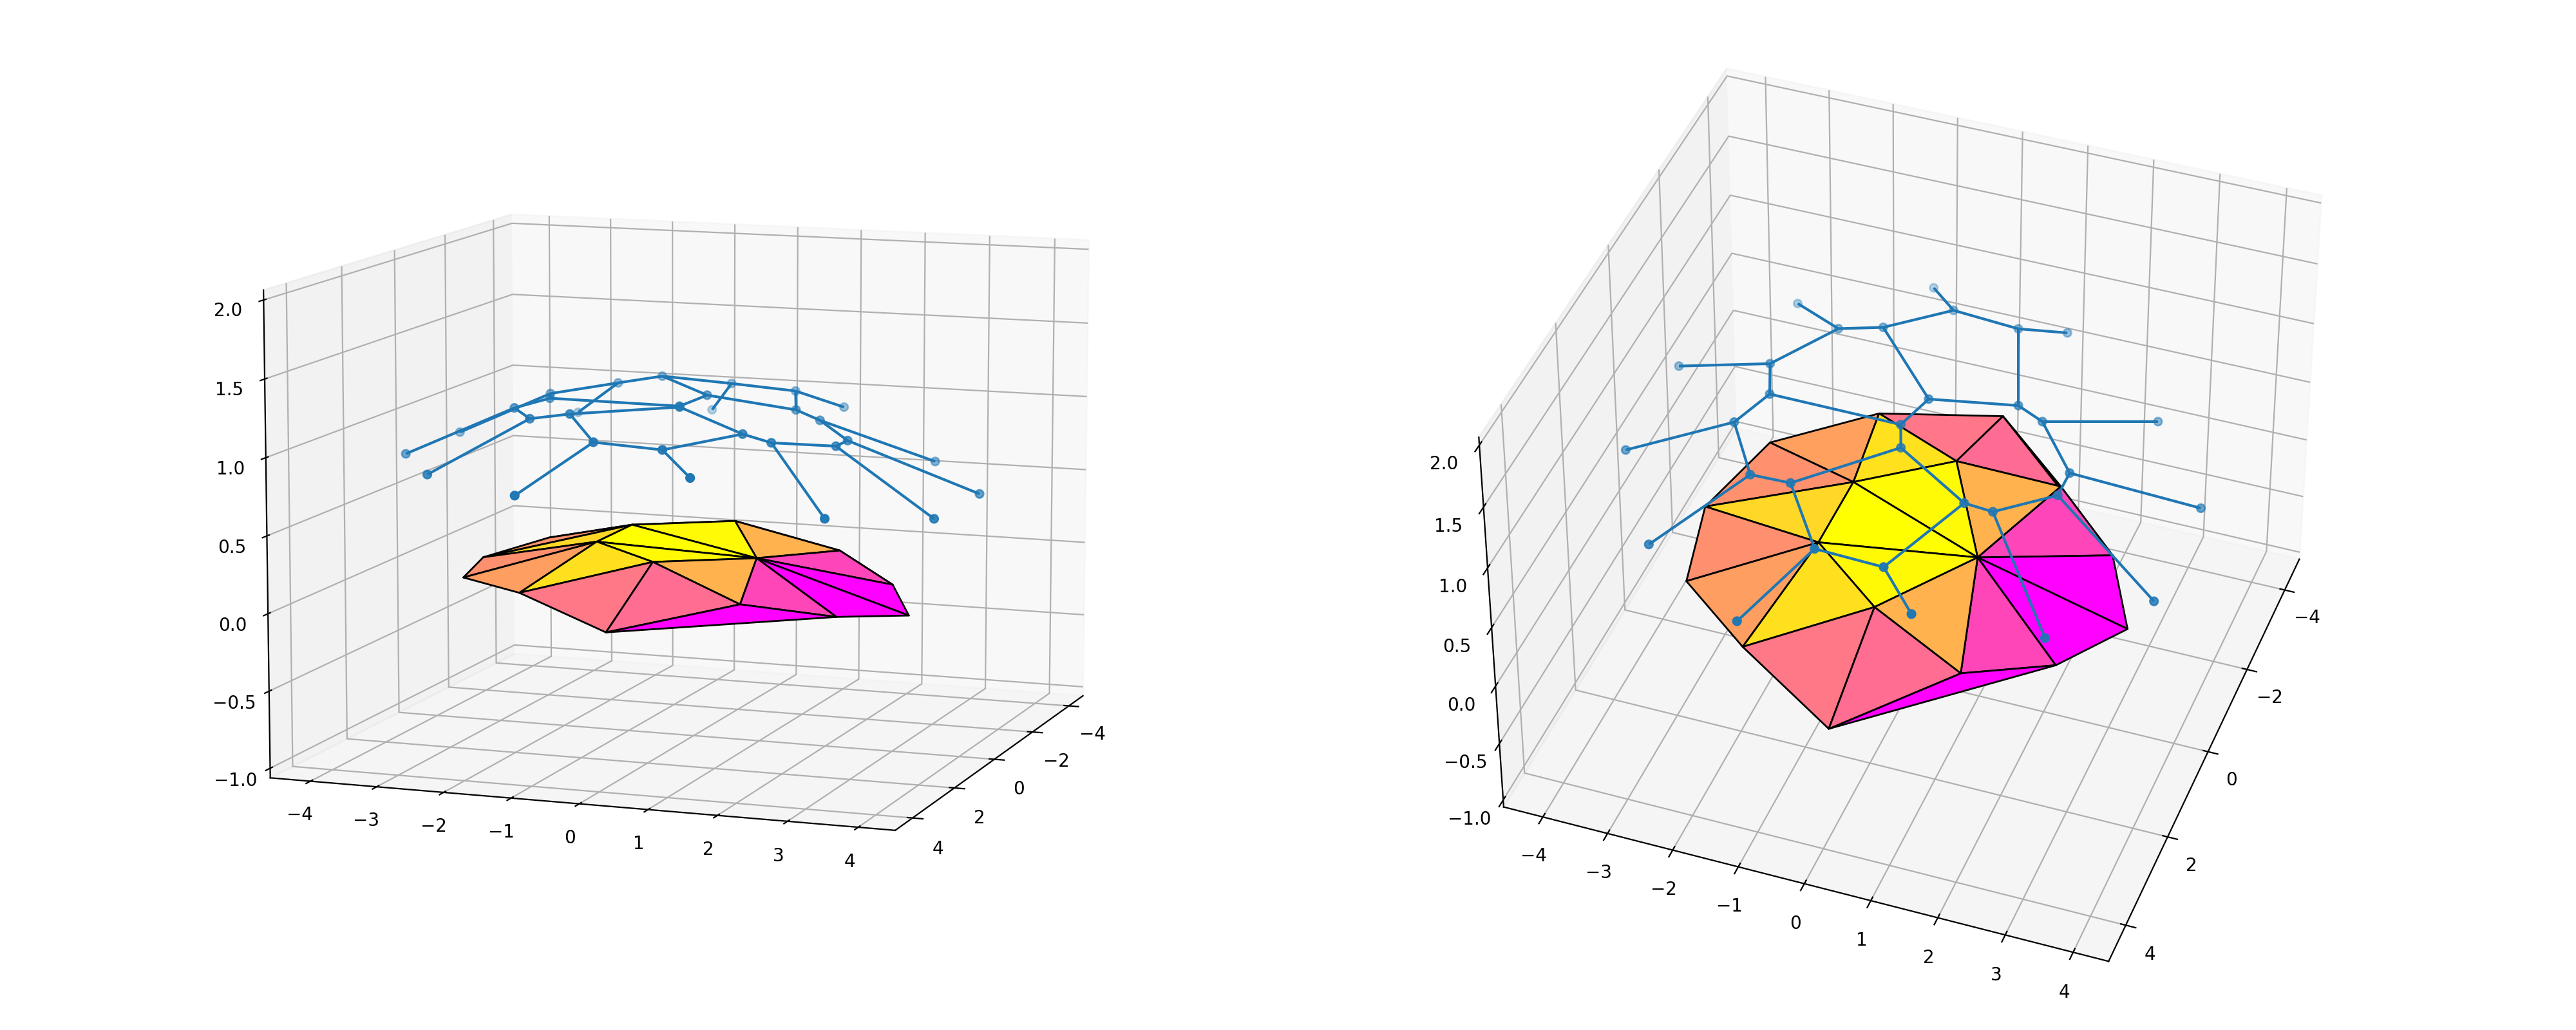
\includegraphics[width=0.69\textwidth]{kink/kink0.95_0.8_1.52_10_plot.png}
        \caption{Sheet shape when $\phi_0=0.95$, $\psi_0=0.8$, $\ell_0=1.52$.}
        \label{subfig:kink_out}
    \end{subfigure}
    \caption{Cell sheet geometry with a node of degree 7. The graph topology is affected in the sheet interior (subfigure \ref{subfig:kink_graph}). This minor change has substantial effects on the sheet geometry (subfigures \ref{subfig:kink_in}, \ref{subfig:kink_out}).}
    \label{fig:kink}
\end{figure}

\begin{figure}[htbp]
    \centering
    \begin{subfigure}[b]{\textwidth}
        \centering
        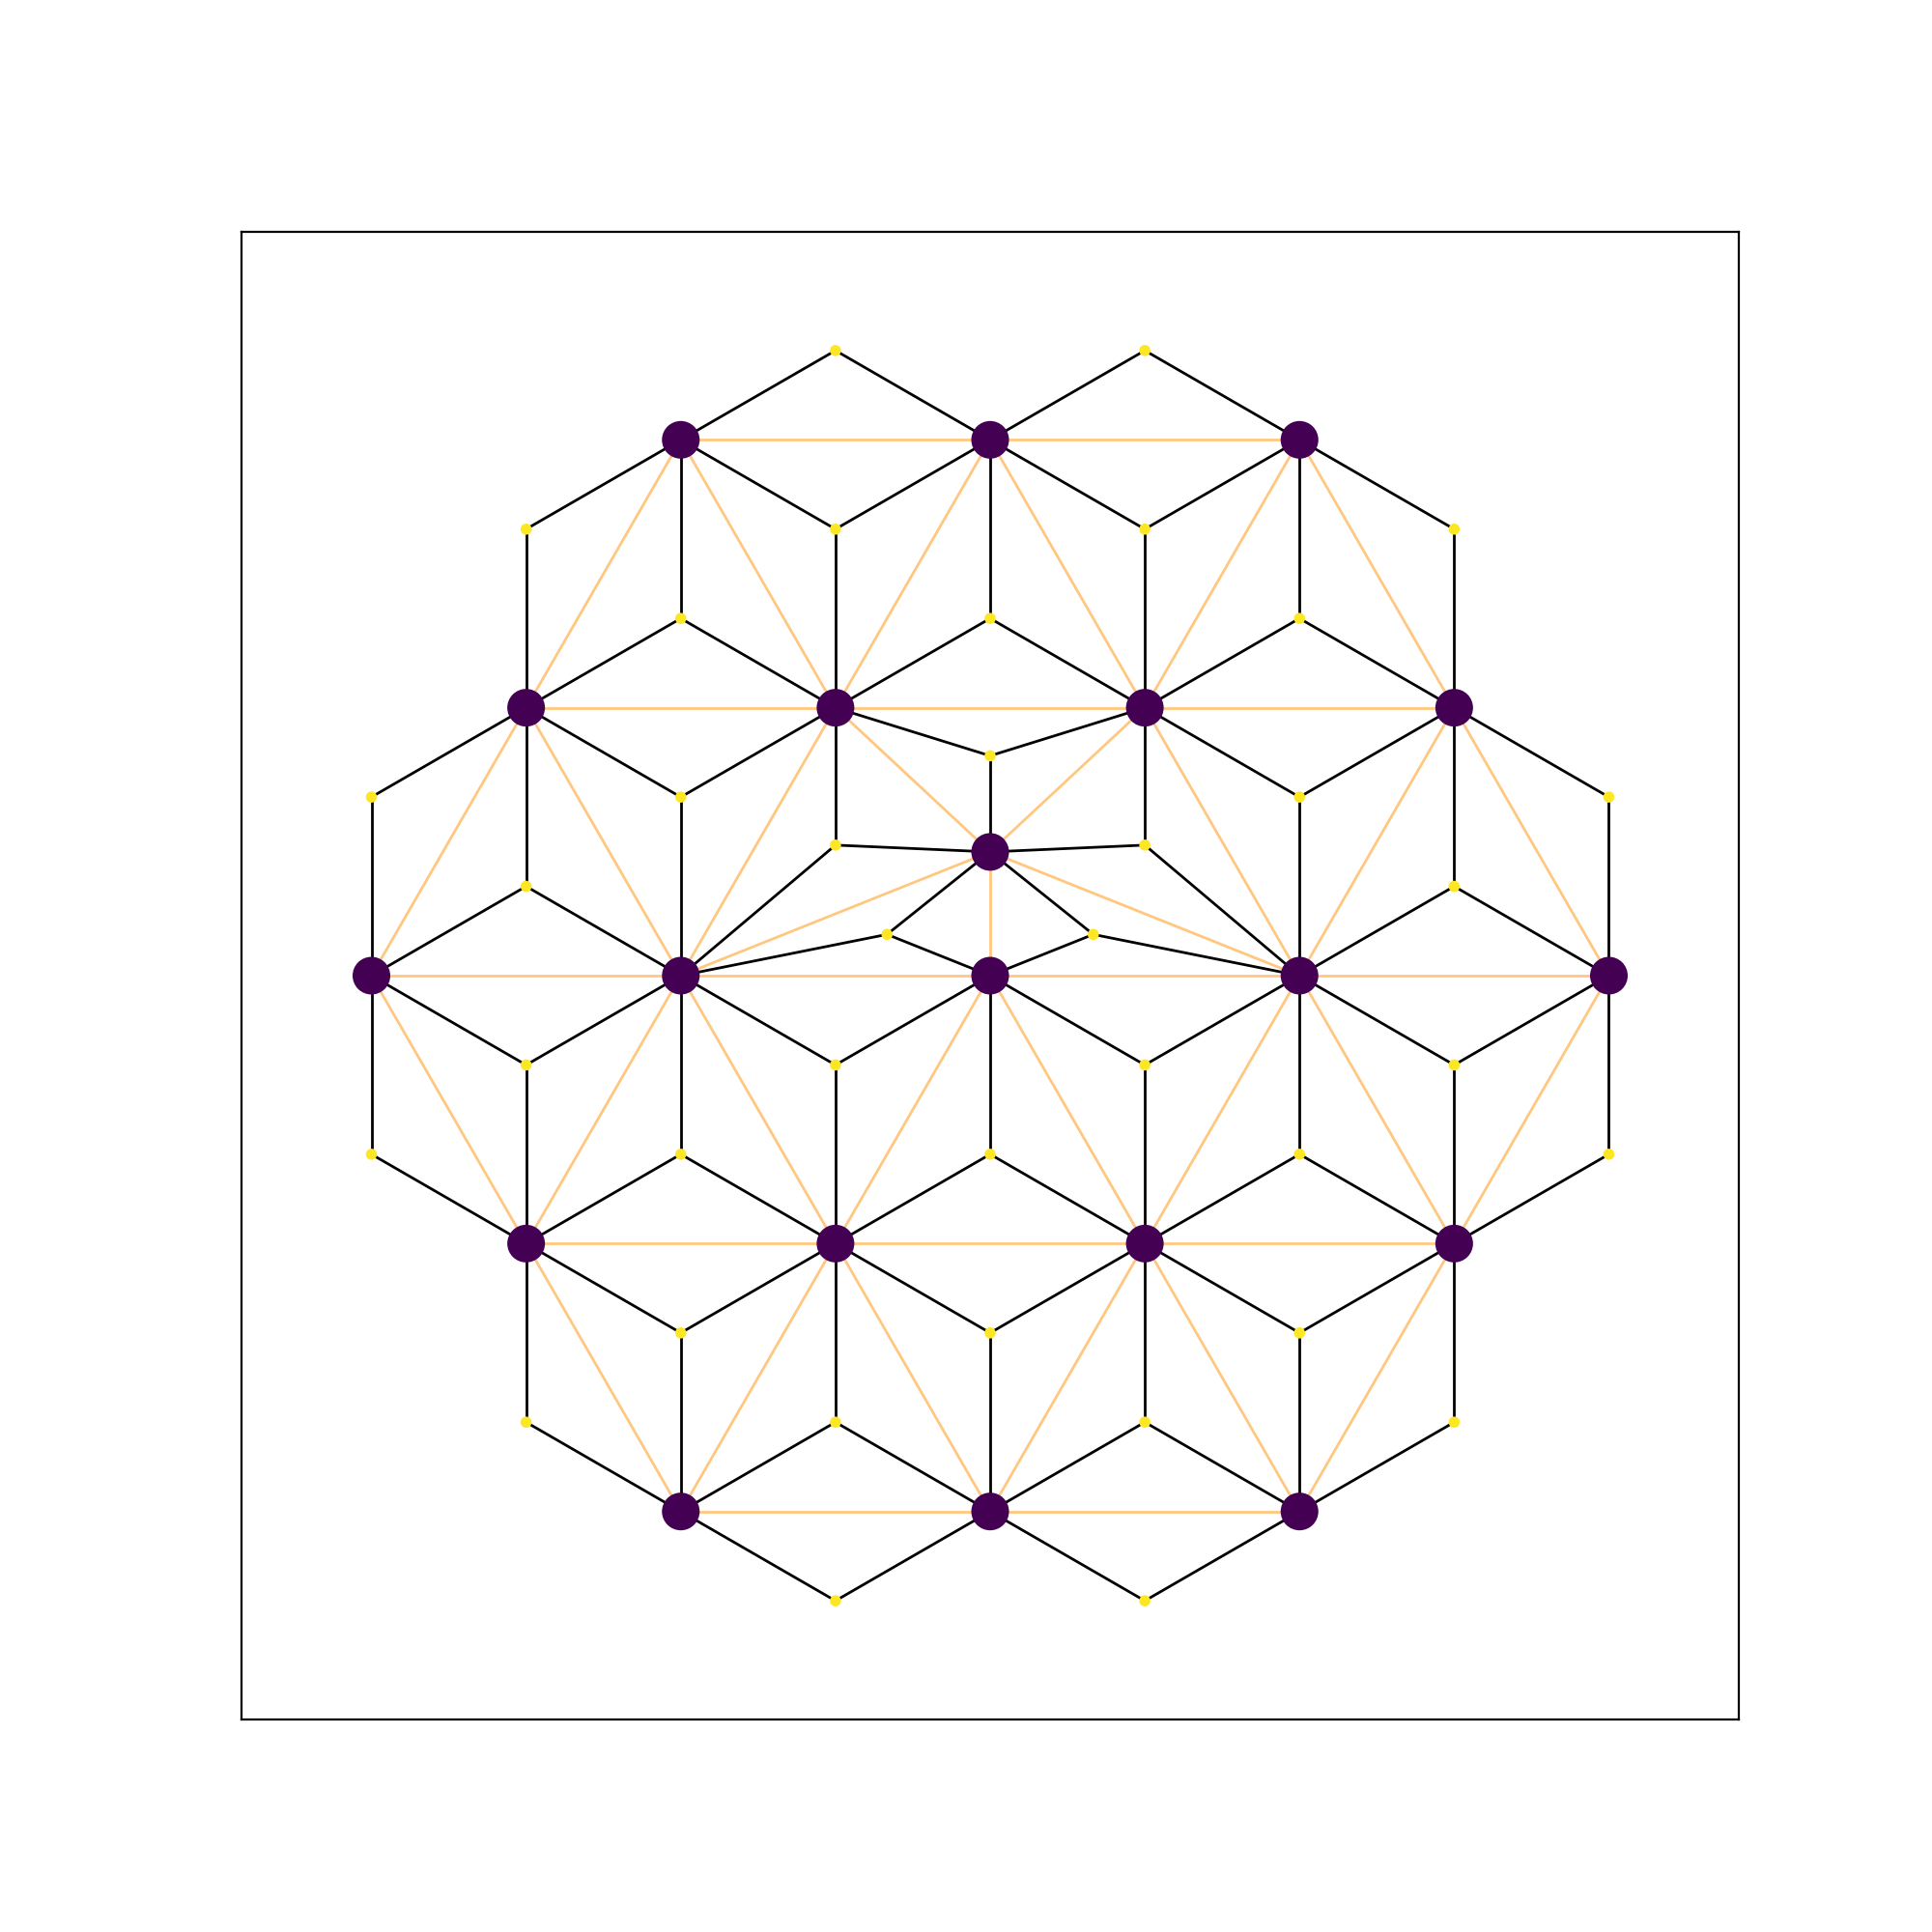
\includegraphics[width=0.5\textwidth]{bump/bump_graph.png}
        \caption{Initial lattice drawn as in Figure \ref{fig:layout_init}.}
        \label{subfig:bump_graph}
    \end{subfigure}
    \begin{subfigure}[b]{\textwidth}
        \centering
        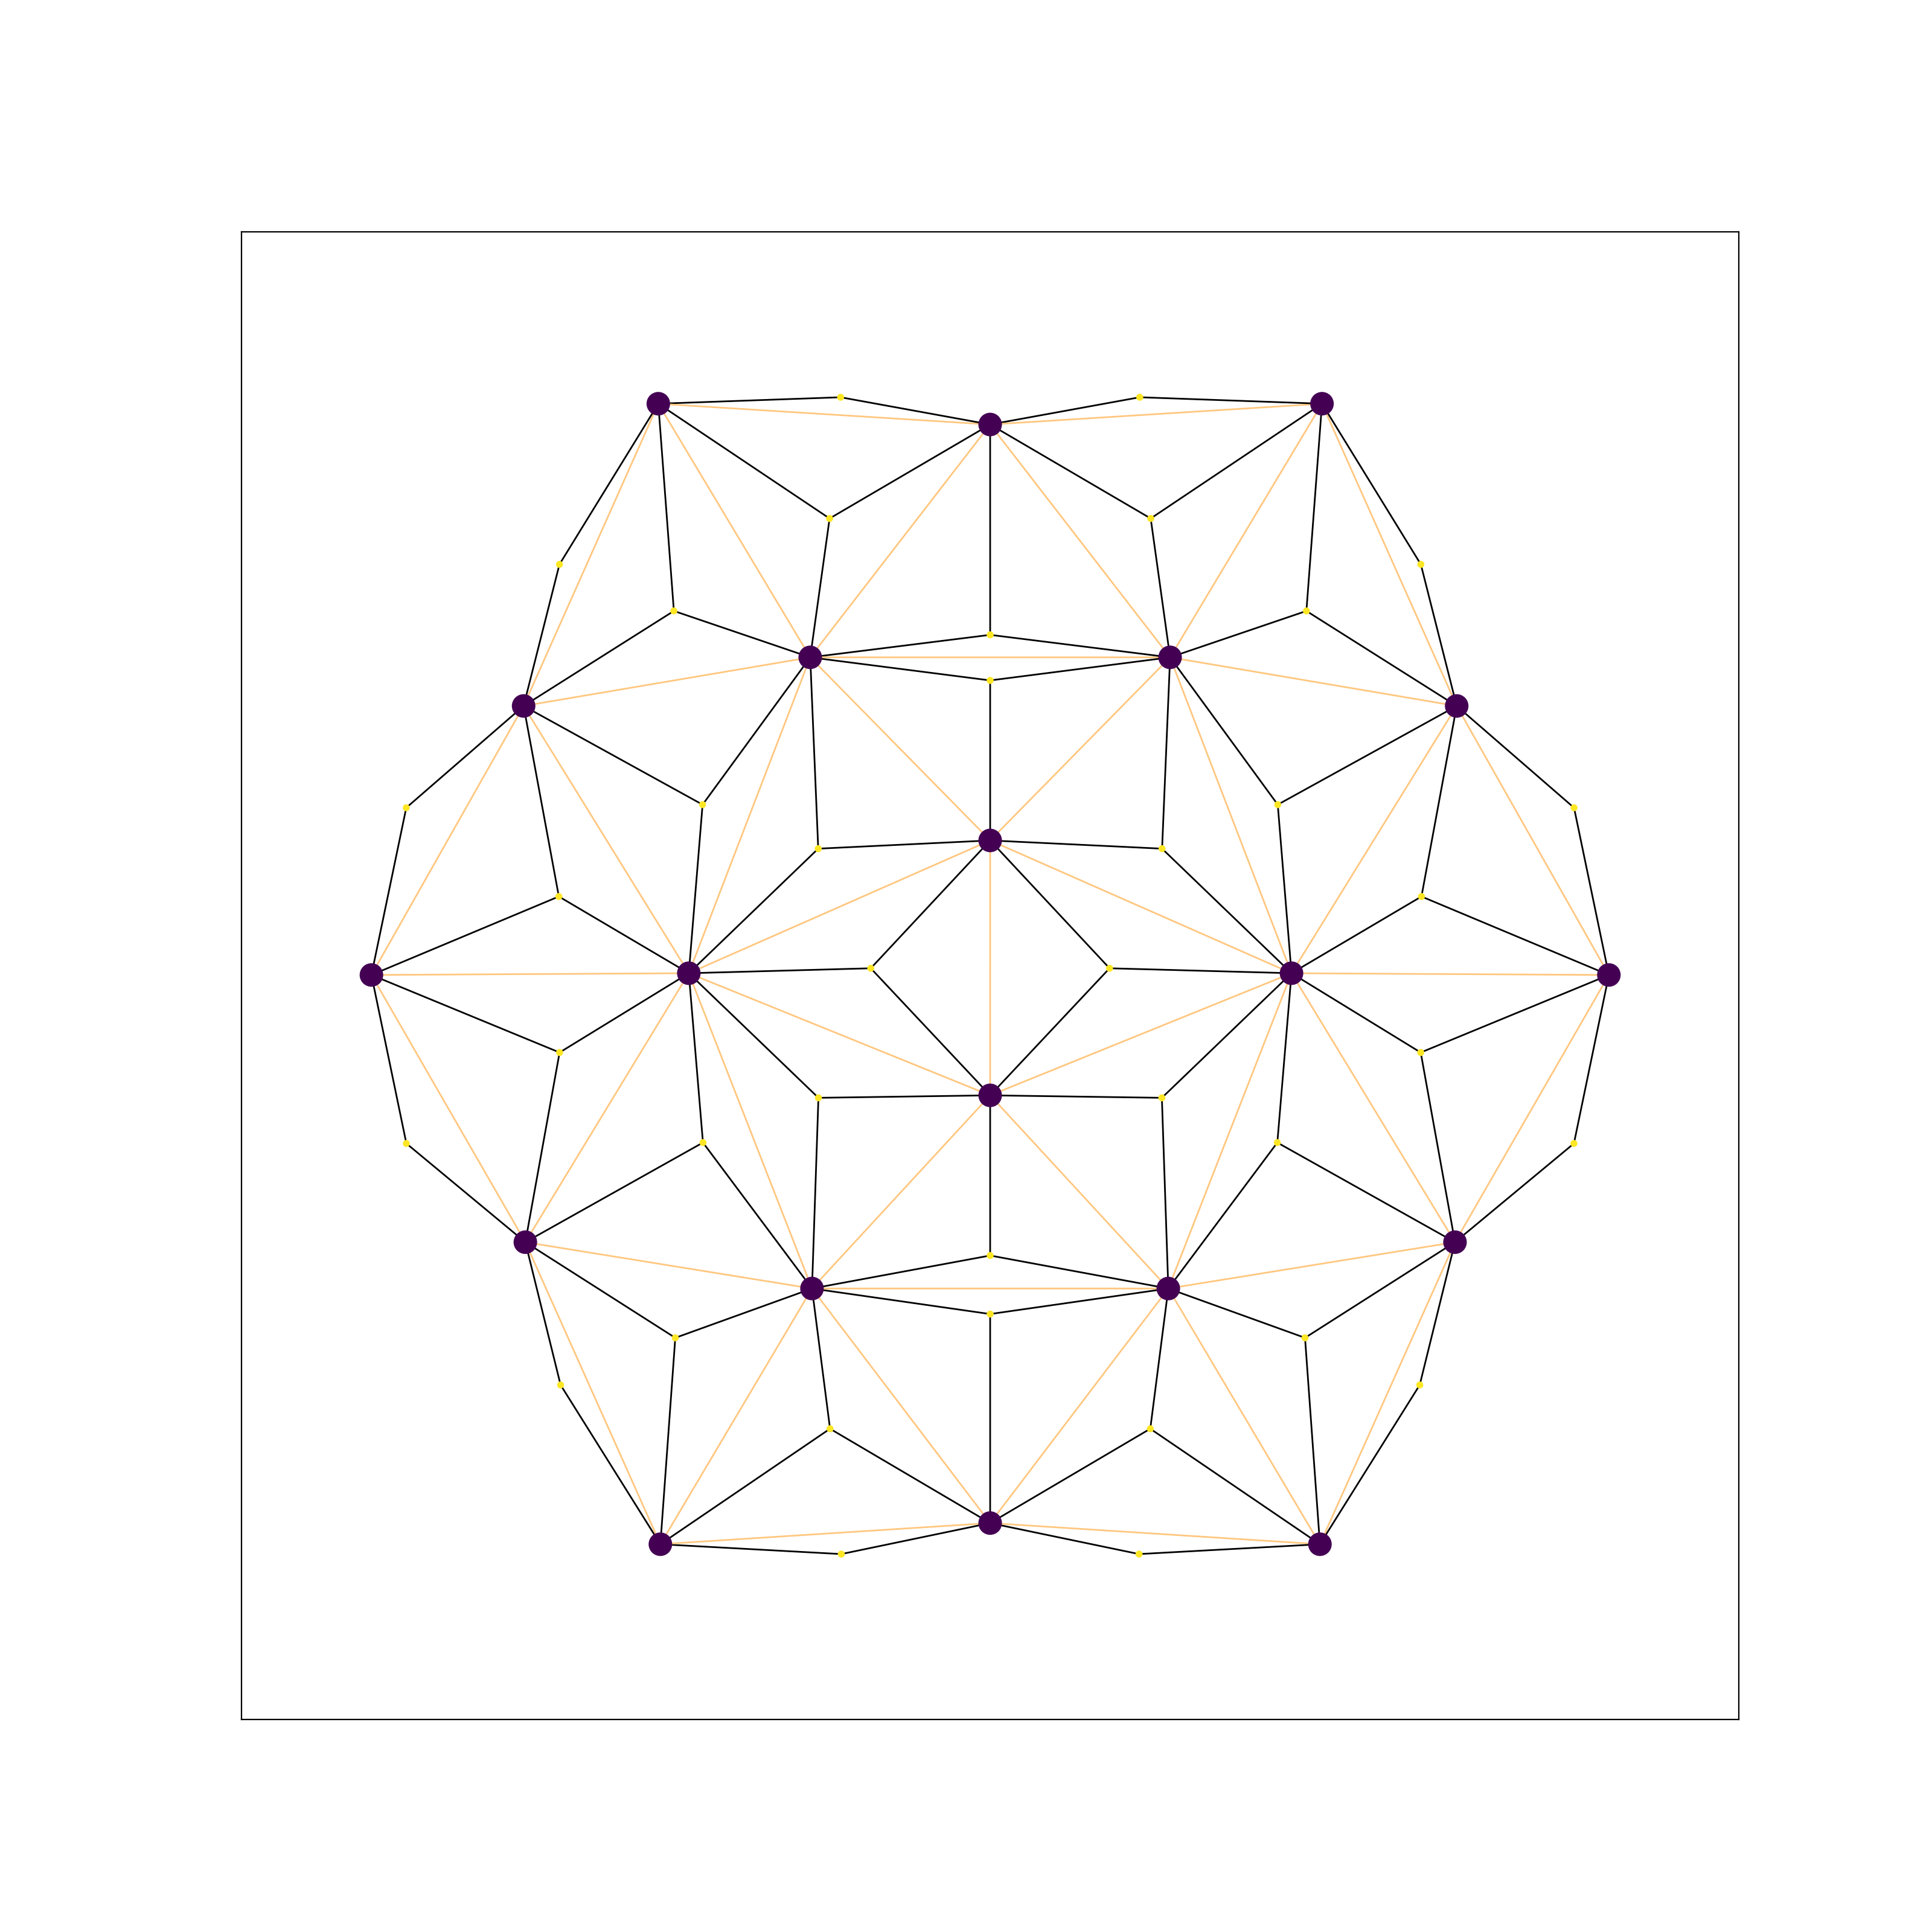
\includegraphics[width=0.3\textwidth]{bump/bump0.8_0.8_1.52_10_graph.png}
        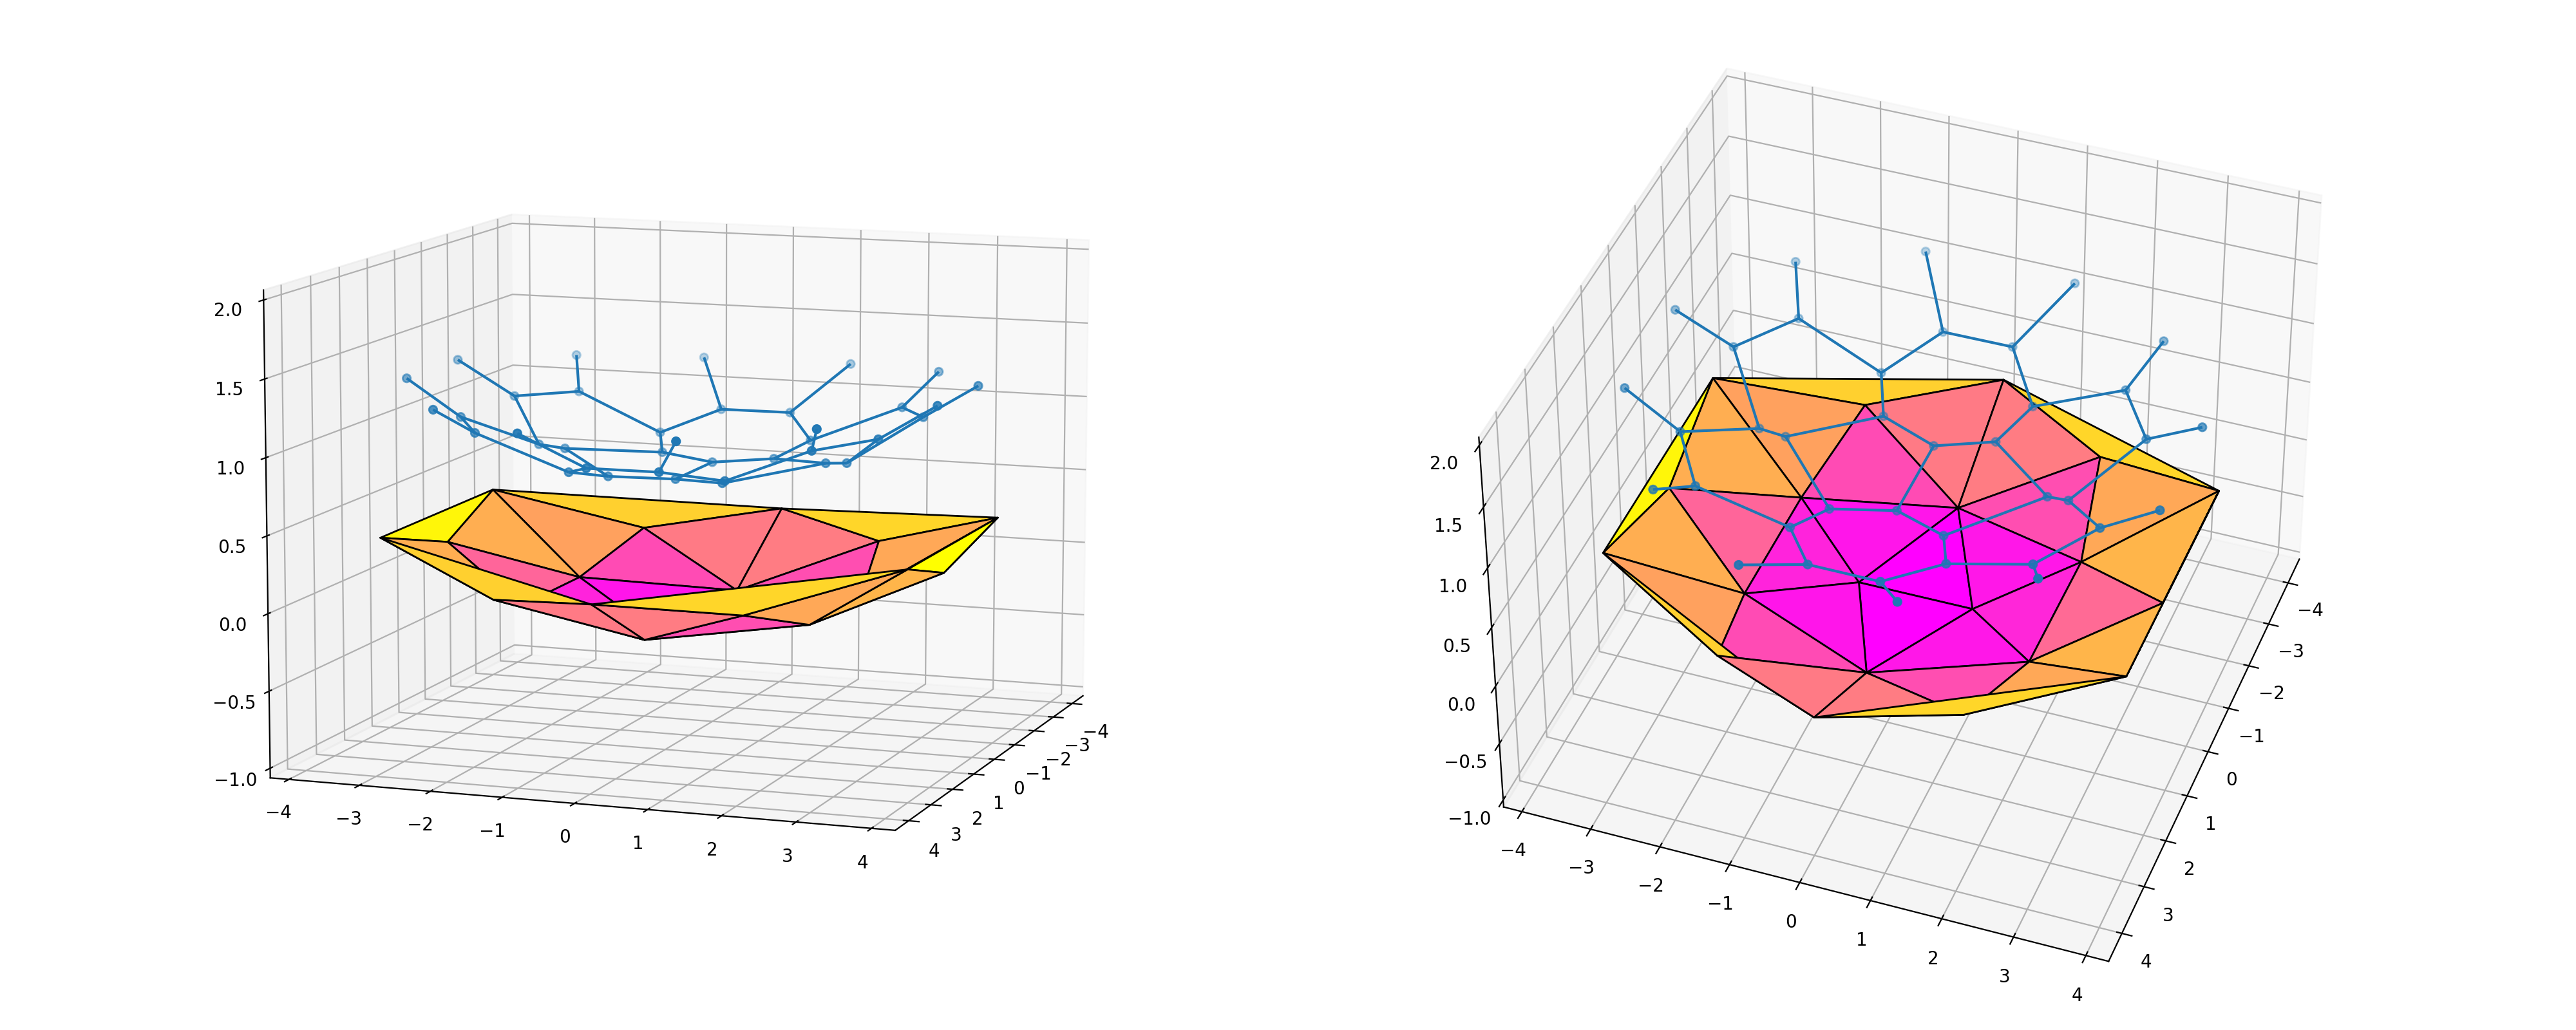
\includegraphics[width=0.69\textwidth]{bump/bump0.8_0.8_1.52_10_plot.png}
        \caption{Sheet shape when $\phi_0=0.8$, $\psi_0=0.8$, $\ell_0=1.52$.}
        \label{subfig:bump_in}
    \end{subfigure}
    \begin{subfigure}[b]{\textwidth}
        \centering
        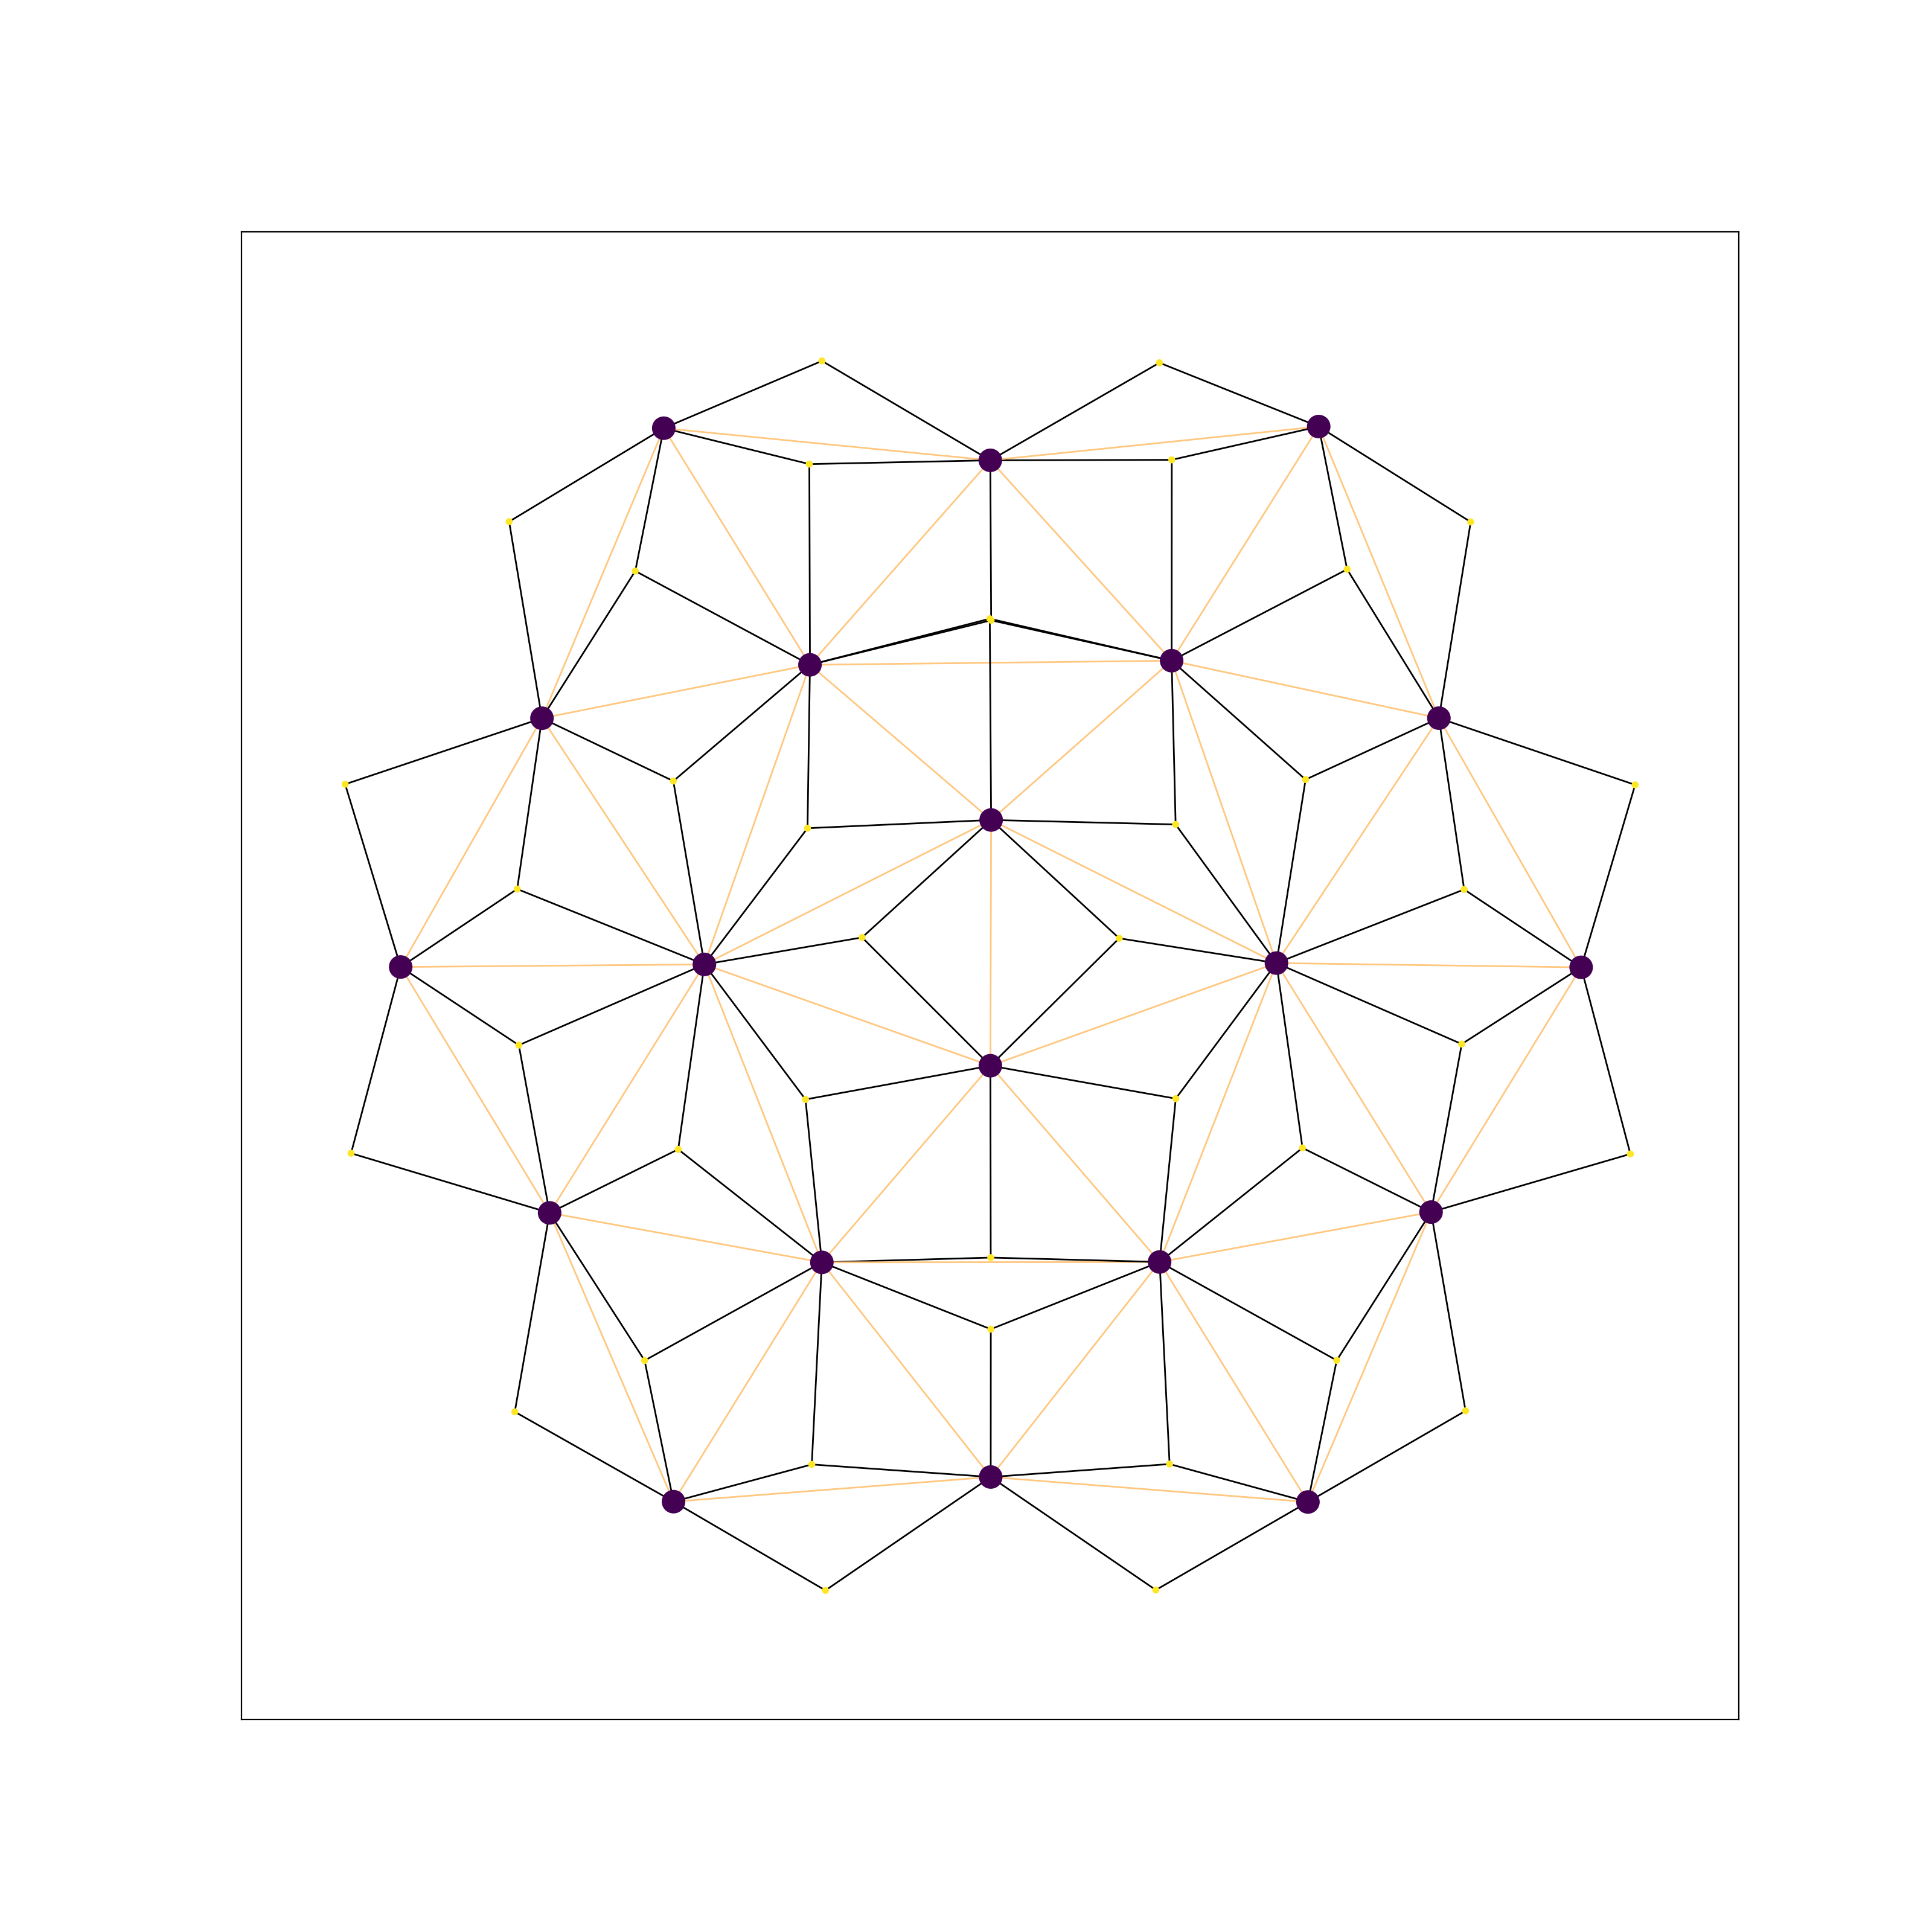
\includegraphics[width=0.3\textwidth]{bump/bump0.95_0.8_1.52_10_graph.png}
        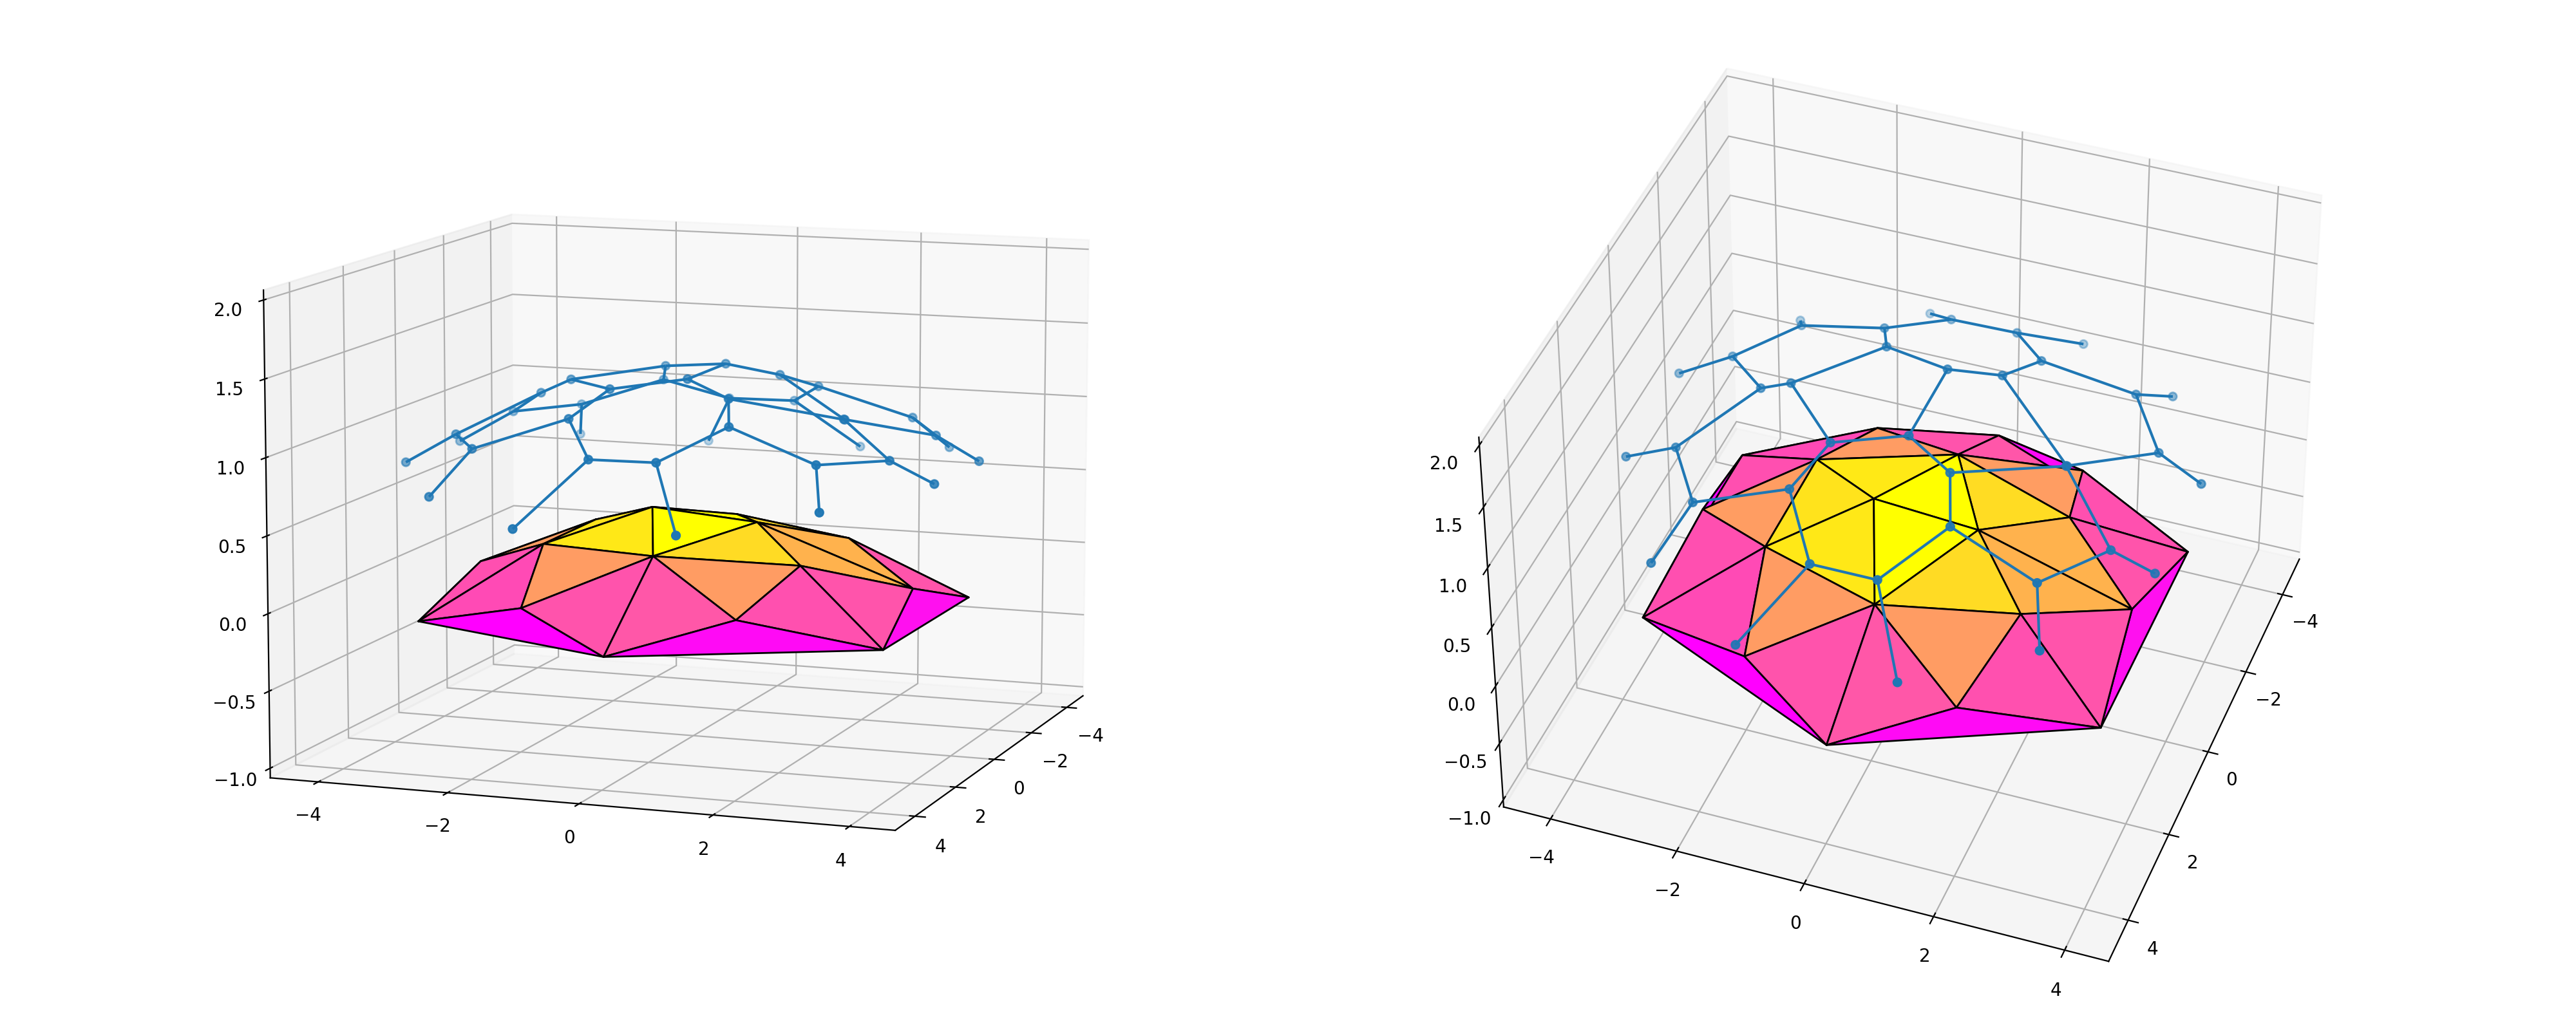
\includegraphics[width=0.69\textwidth]{bump/bump0.95_0.8_1.52_10_plot.png}
        \caption{Sheet shape when $\phi_0=0.95$, $\psi_0=0.8$, $\ell_0=1.52$.}
        \label{subfig:bump_out}
    \end{subfigure}
    \caption{Cell sheet geometry with a node of degree 7. The graph topology is affected in the sheet interior (subfigure \ref{subfig:bump_graph}). This minor change has substantial effects on the sheet geometry (subfigures \ref{subfig:bump_in}, \ref{subfig:bump_out}).}
    \label{fig:bump}
\end{figure}

\subsection{Larger cell sheets}

If if inverting a sheet of cells involves flattening it out at the edges, then a small sheet will be able to do this easier than a large one. This is because the cells on the outside have to stretch their collars less if the sheet is smaller when they flatten out. 

\begin{figure}[htbp]
    \centering
    \begin{subfigure}[b]{\textwidth}
        \centering
        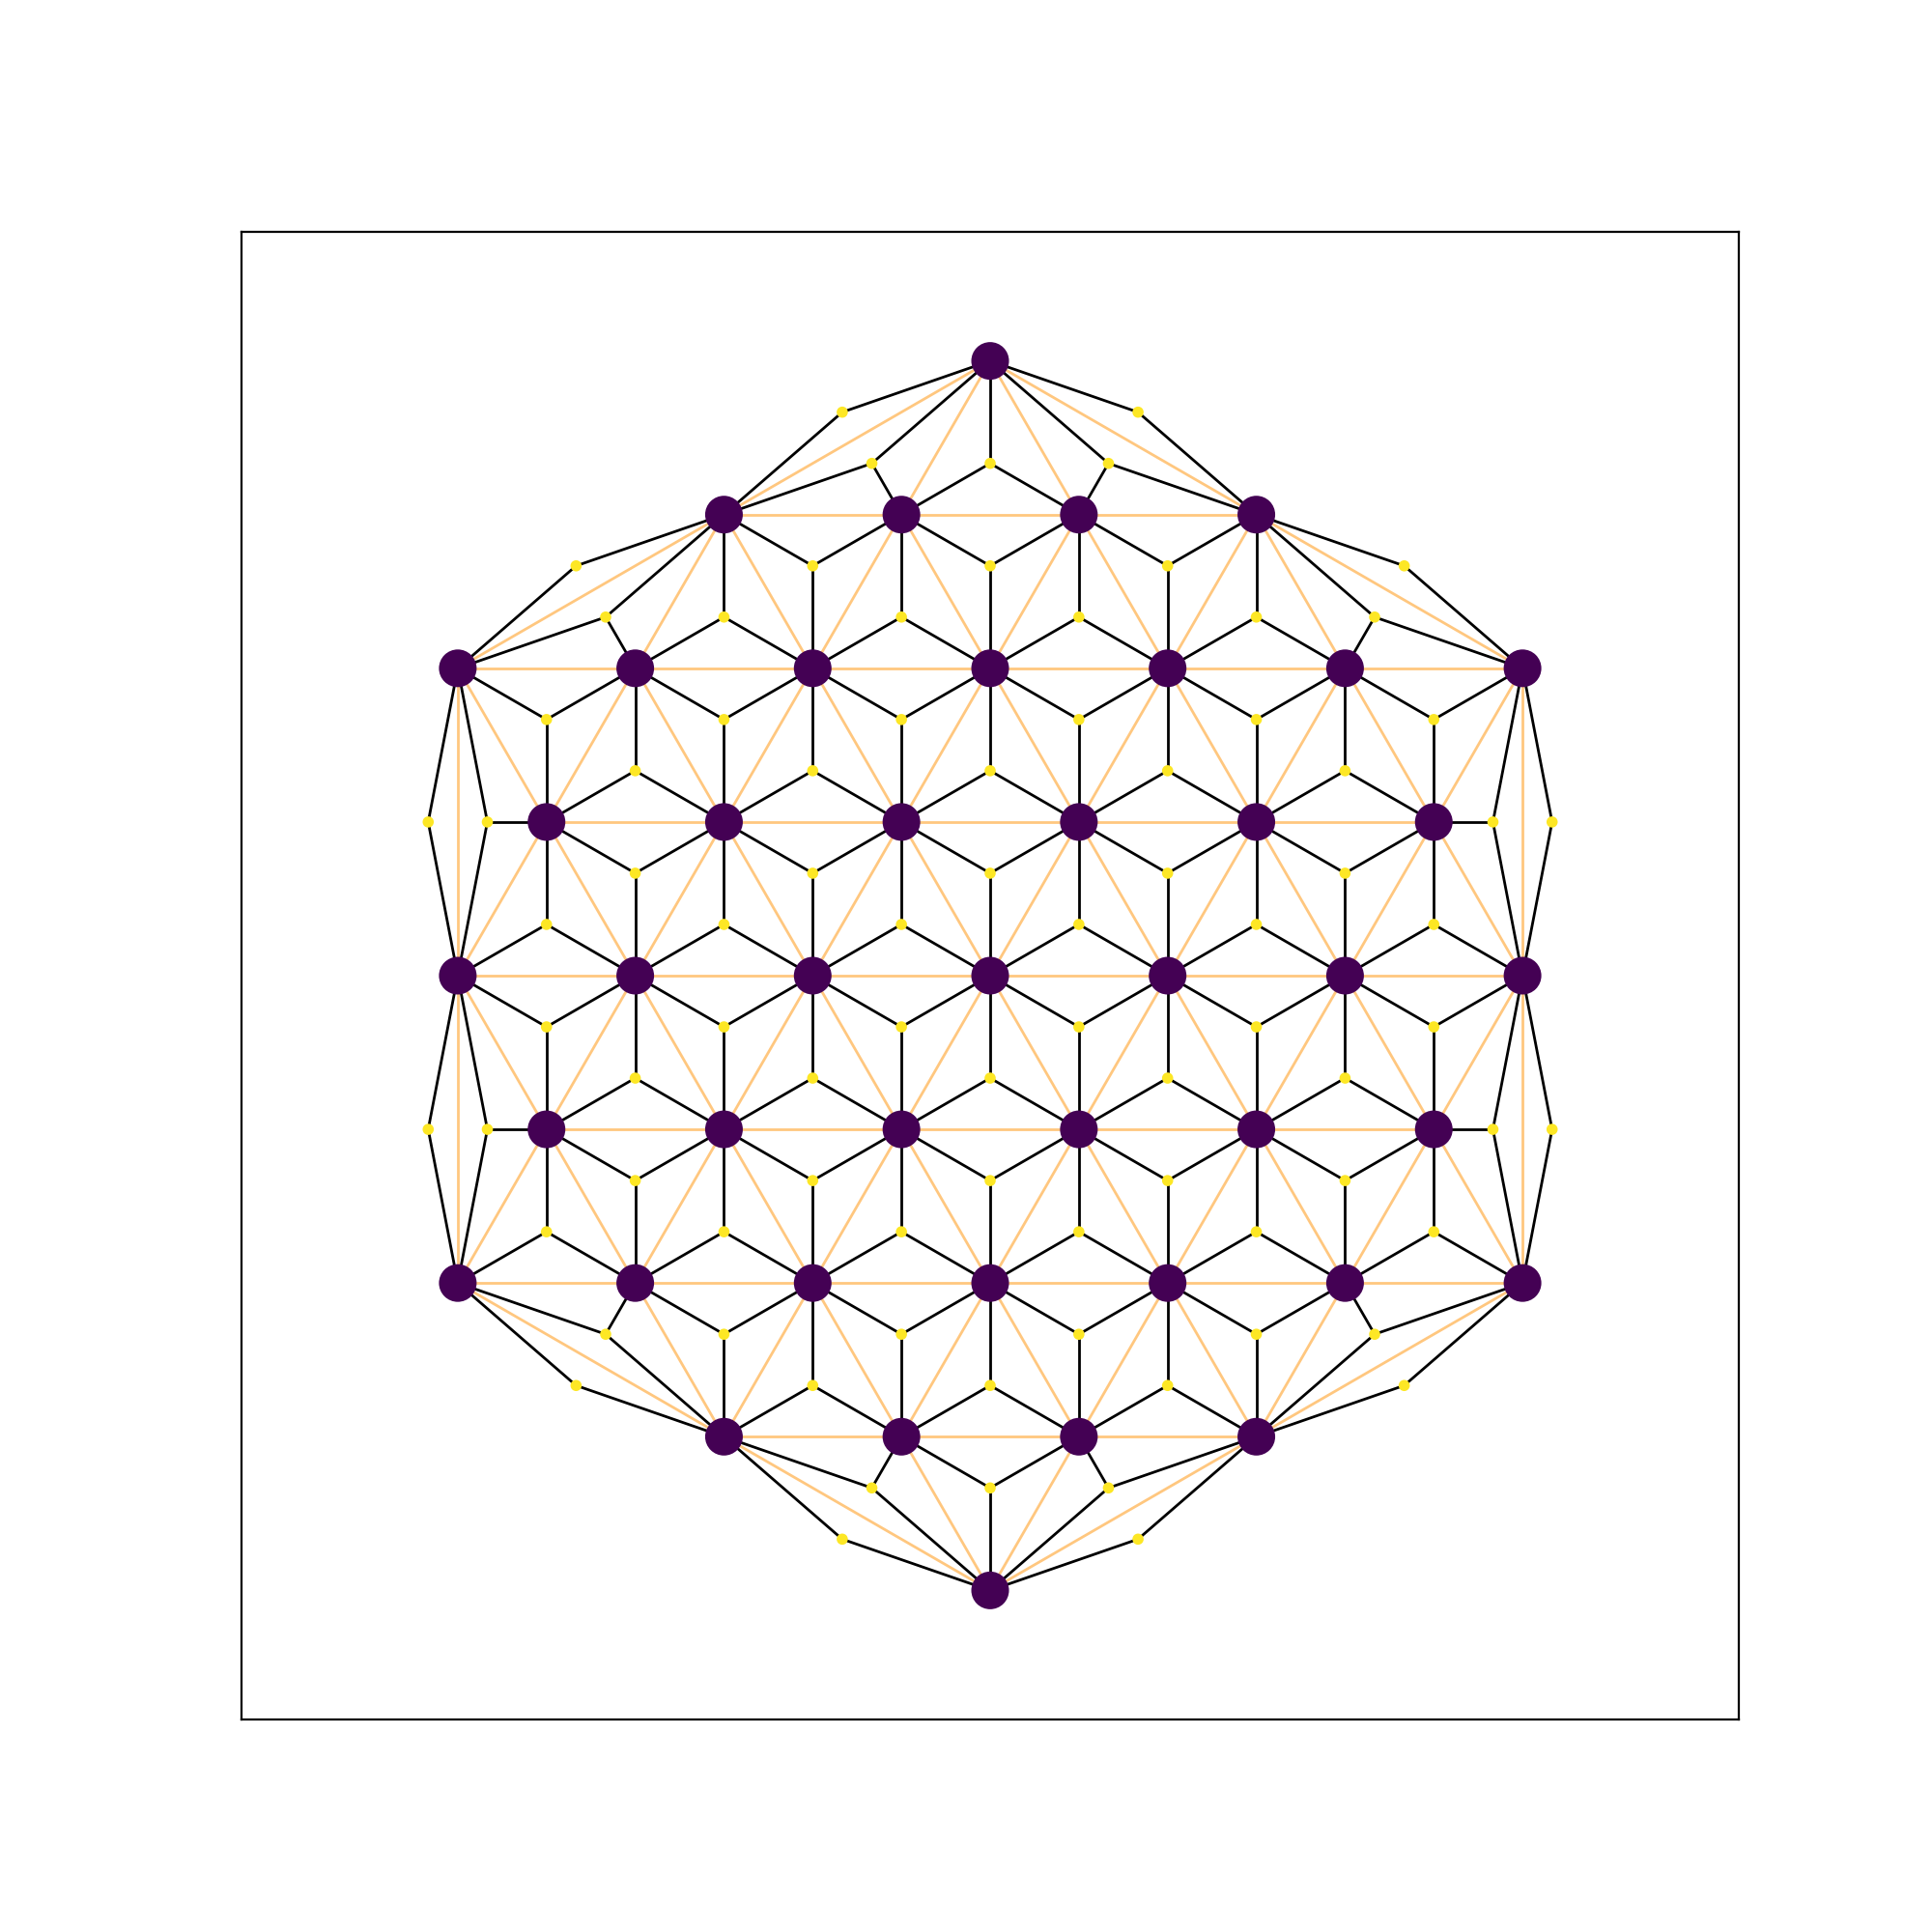
\includegraphics[width=0.5\textwidth]{hexbig/hexbig_graph.png}
        \caption{Initial lattice drawn as in Figure \ref{fig:layout_init}.}
        \label{subfig:hexbig_graph}
    \end{subfigure}
    \begin{subfigure}[b]{\textwidth}
        \centering
        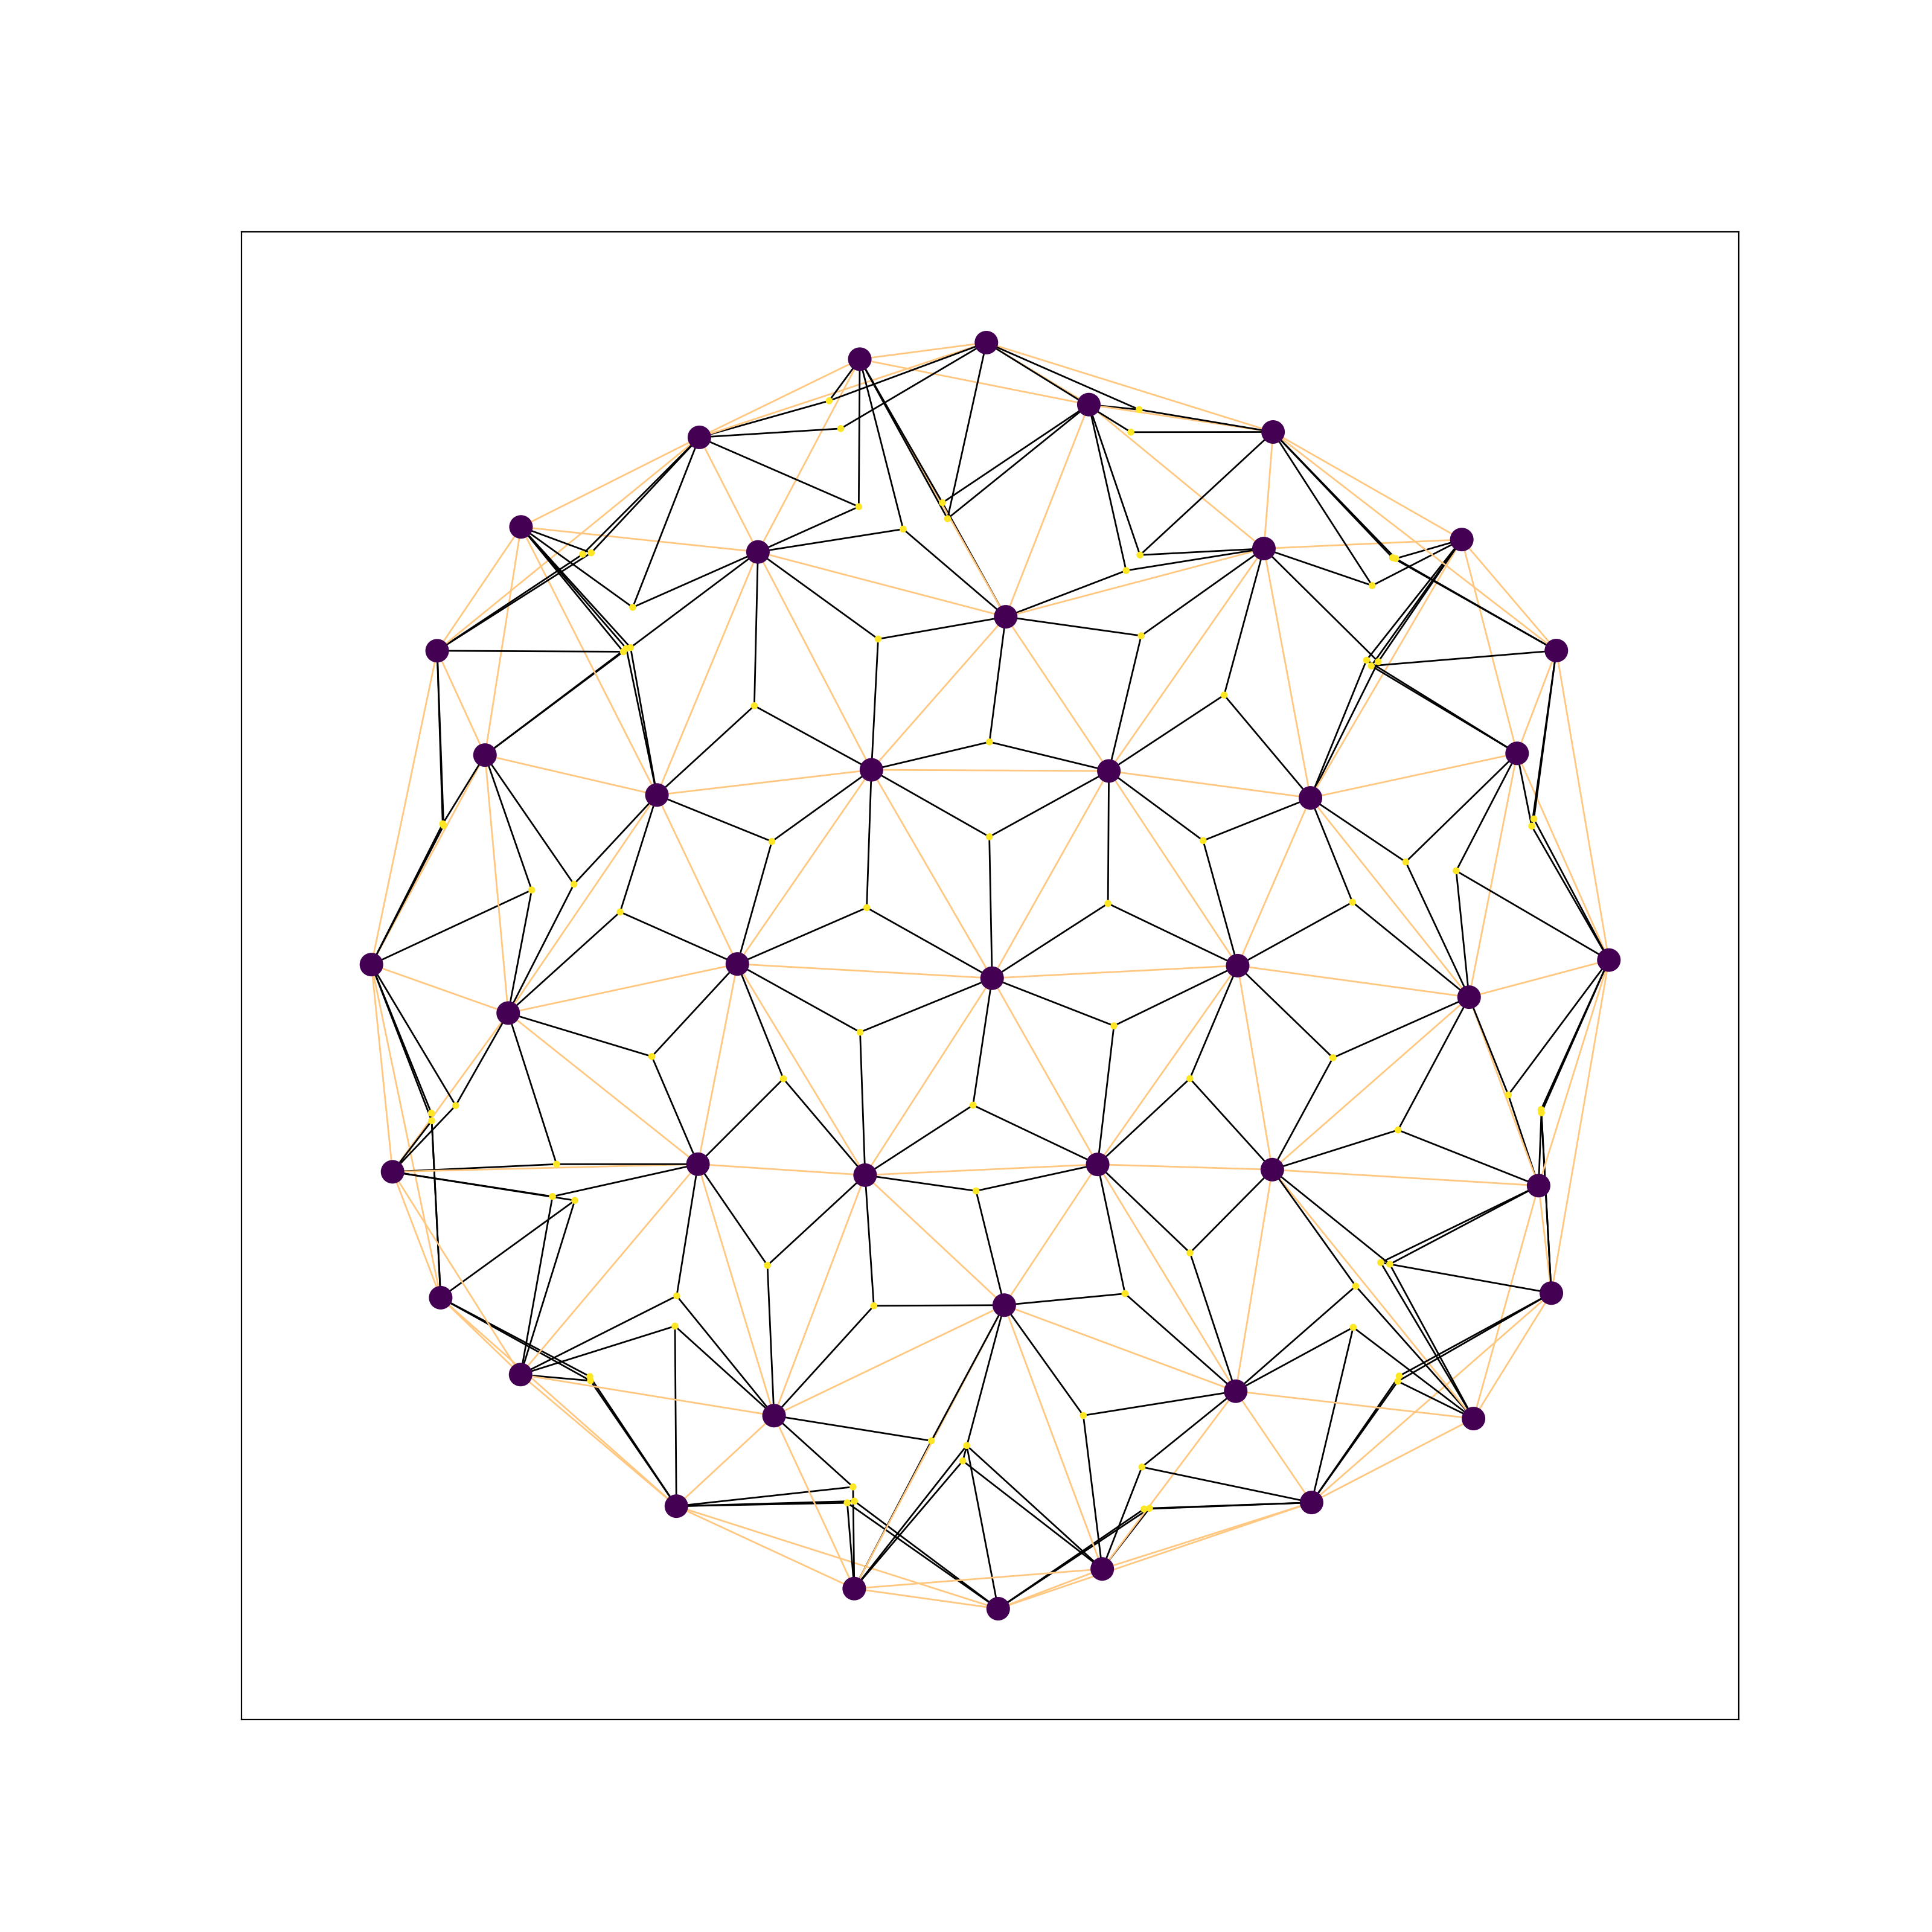
\includegraphics[width=0.3\textwidth]{hexbig/hexbig0.8_0.8_1.35_10_graph.png}
        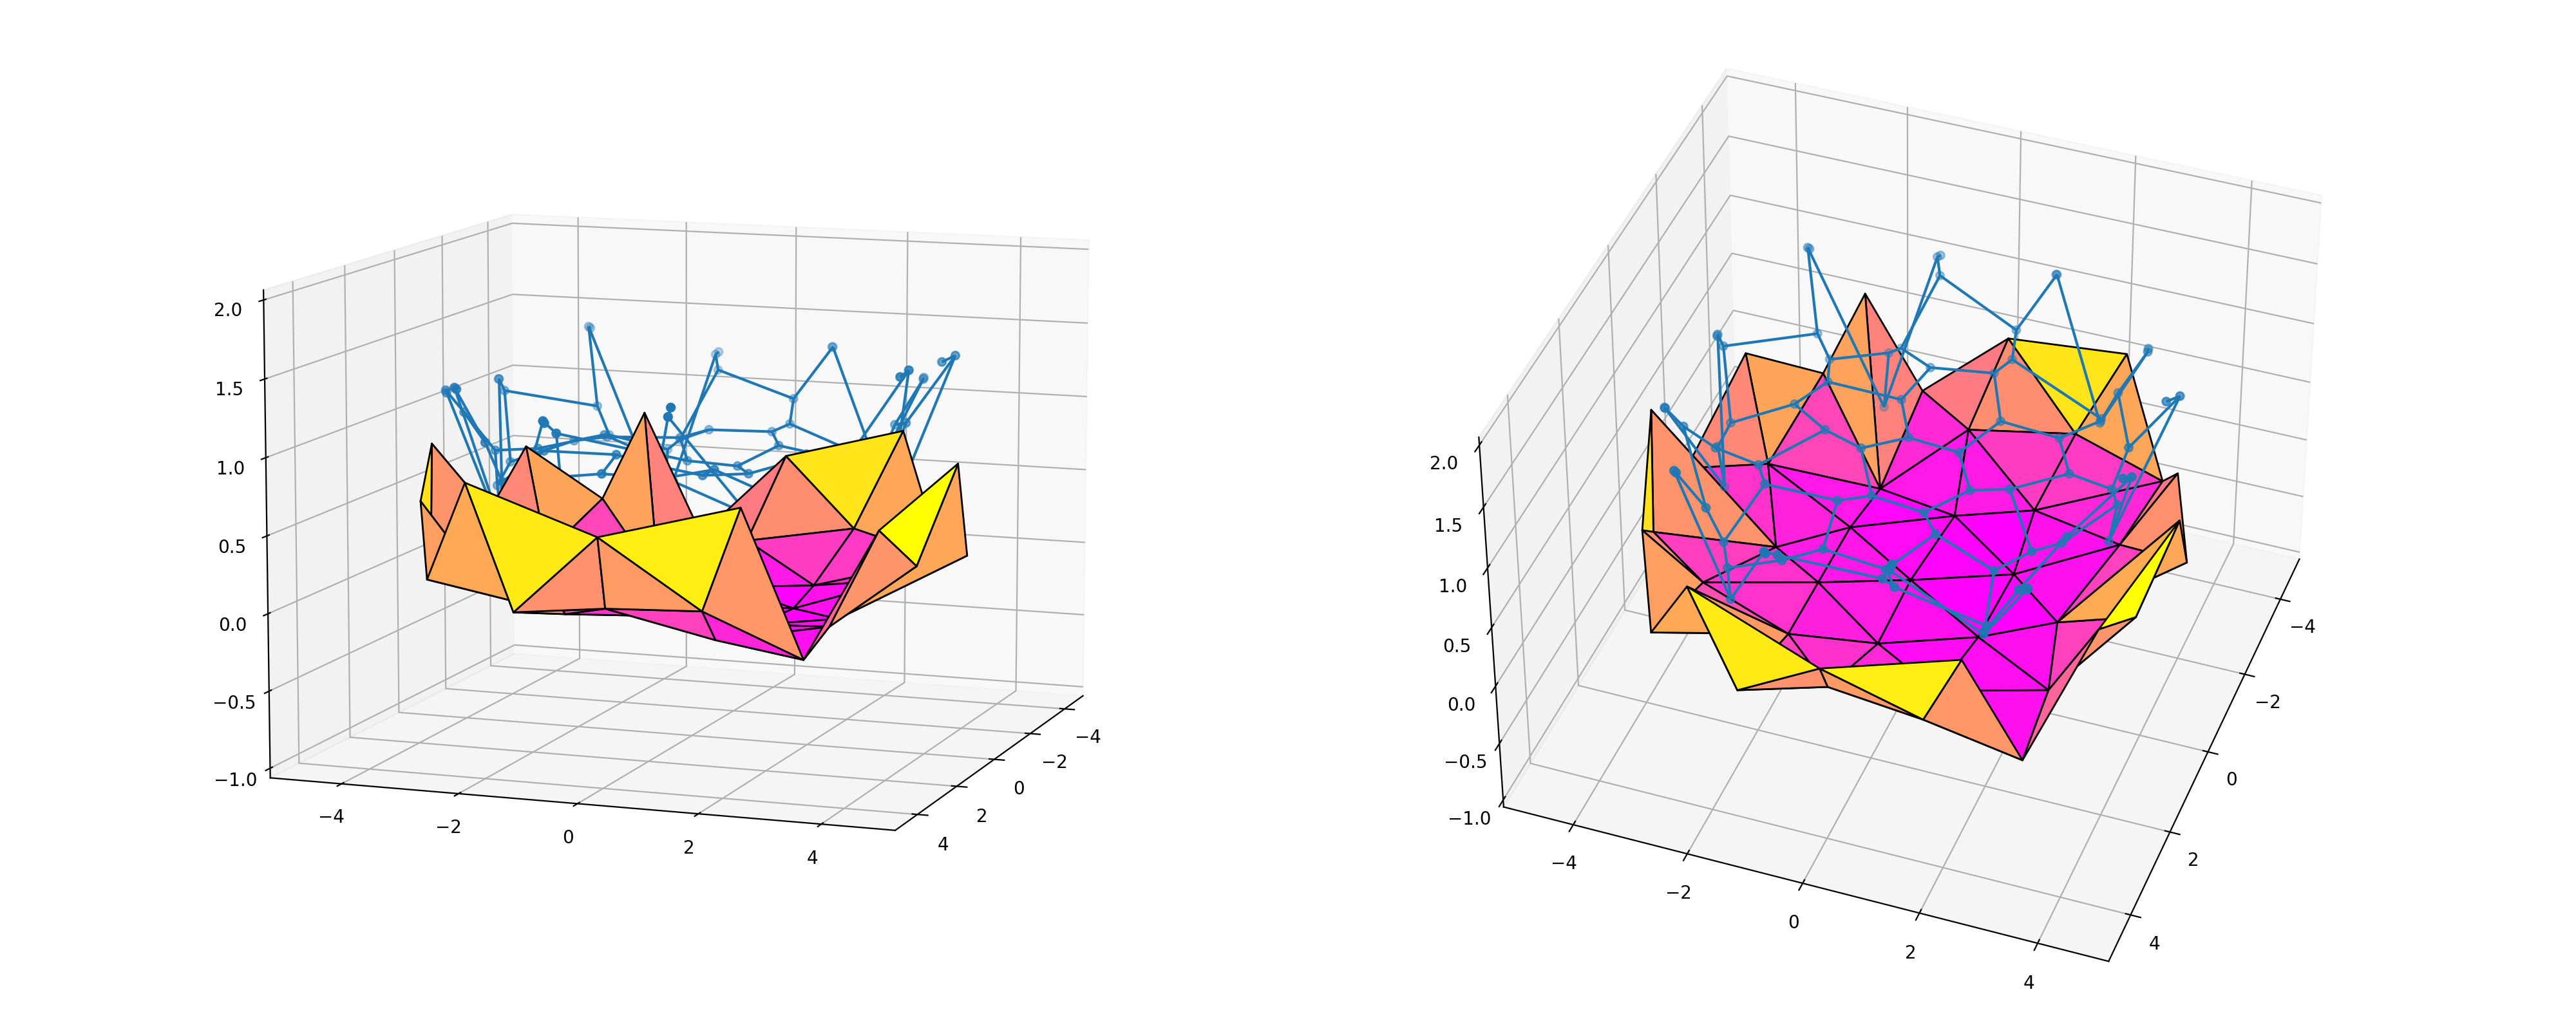
\includegraphics[width=0.69\textwidth]{hexbig/hexbig0.8_0.8_1.35_10_plot.png}
        \caption{Sheet shape when $\phi_0=0.8$, $\psi_0=0.8$, $\ell_0=1.52$.}
        \label{subfig:hexbig_in}
    \end{subfigure}
    \begin{subfigure}[b]{\textwidth}
        \centering
        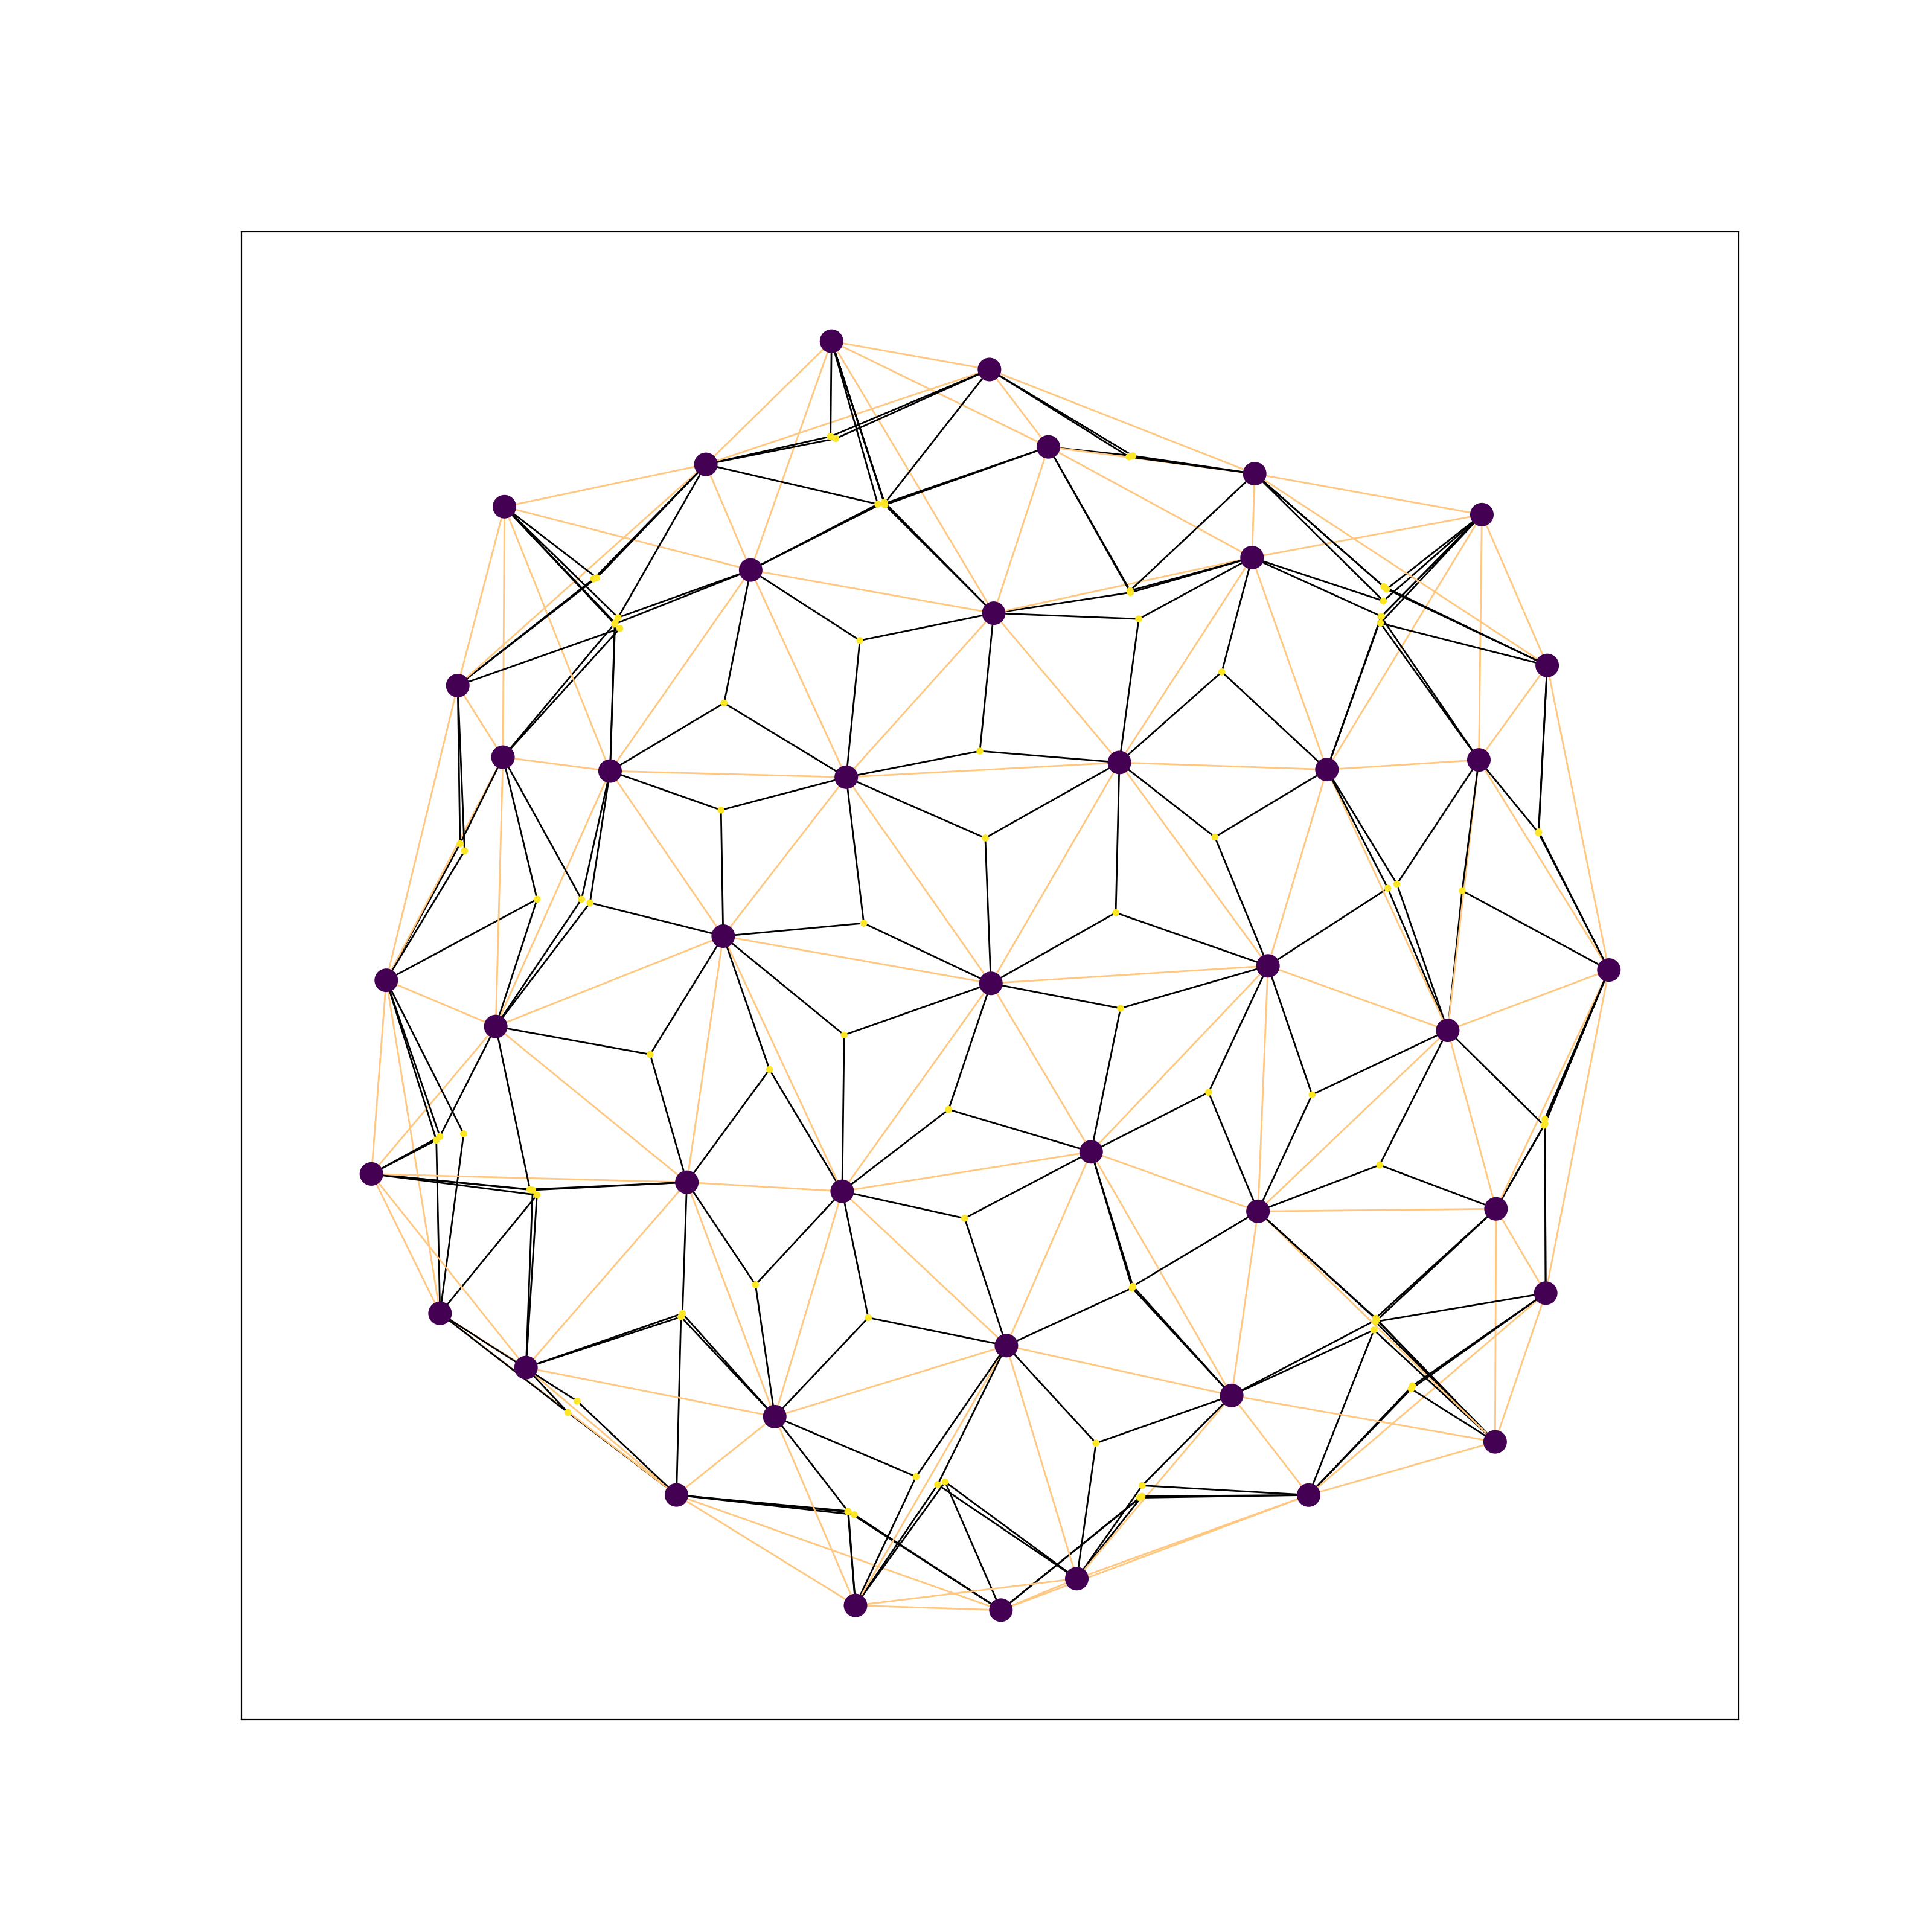
\includegraphics[width=0.3\textwidth]{hexbig/hexbig0.95_0.8_1.35_10_graph.png}
        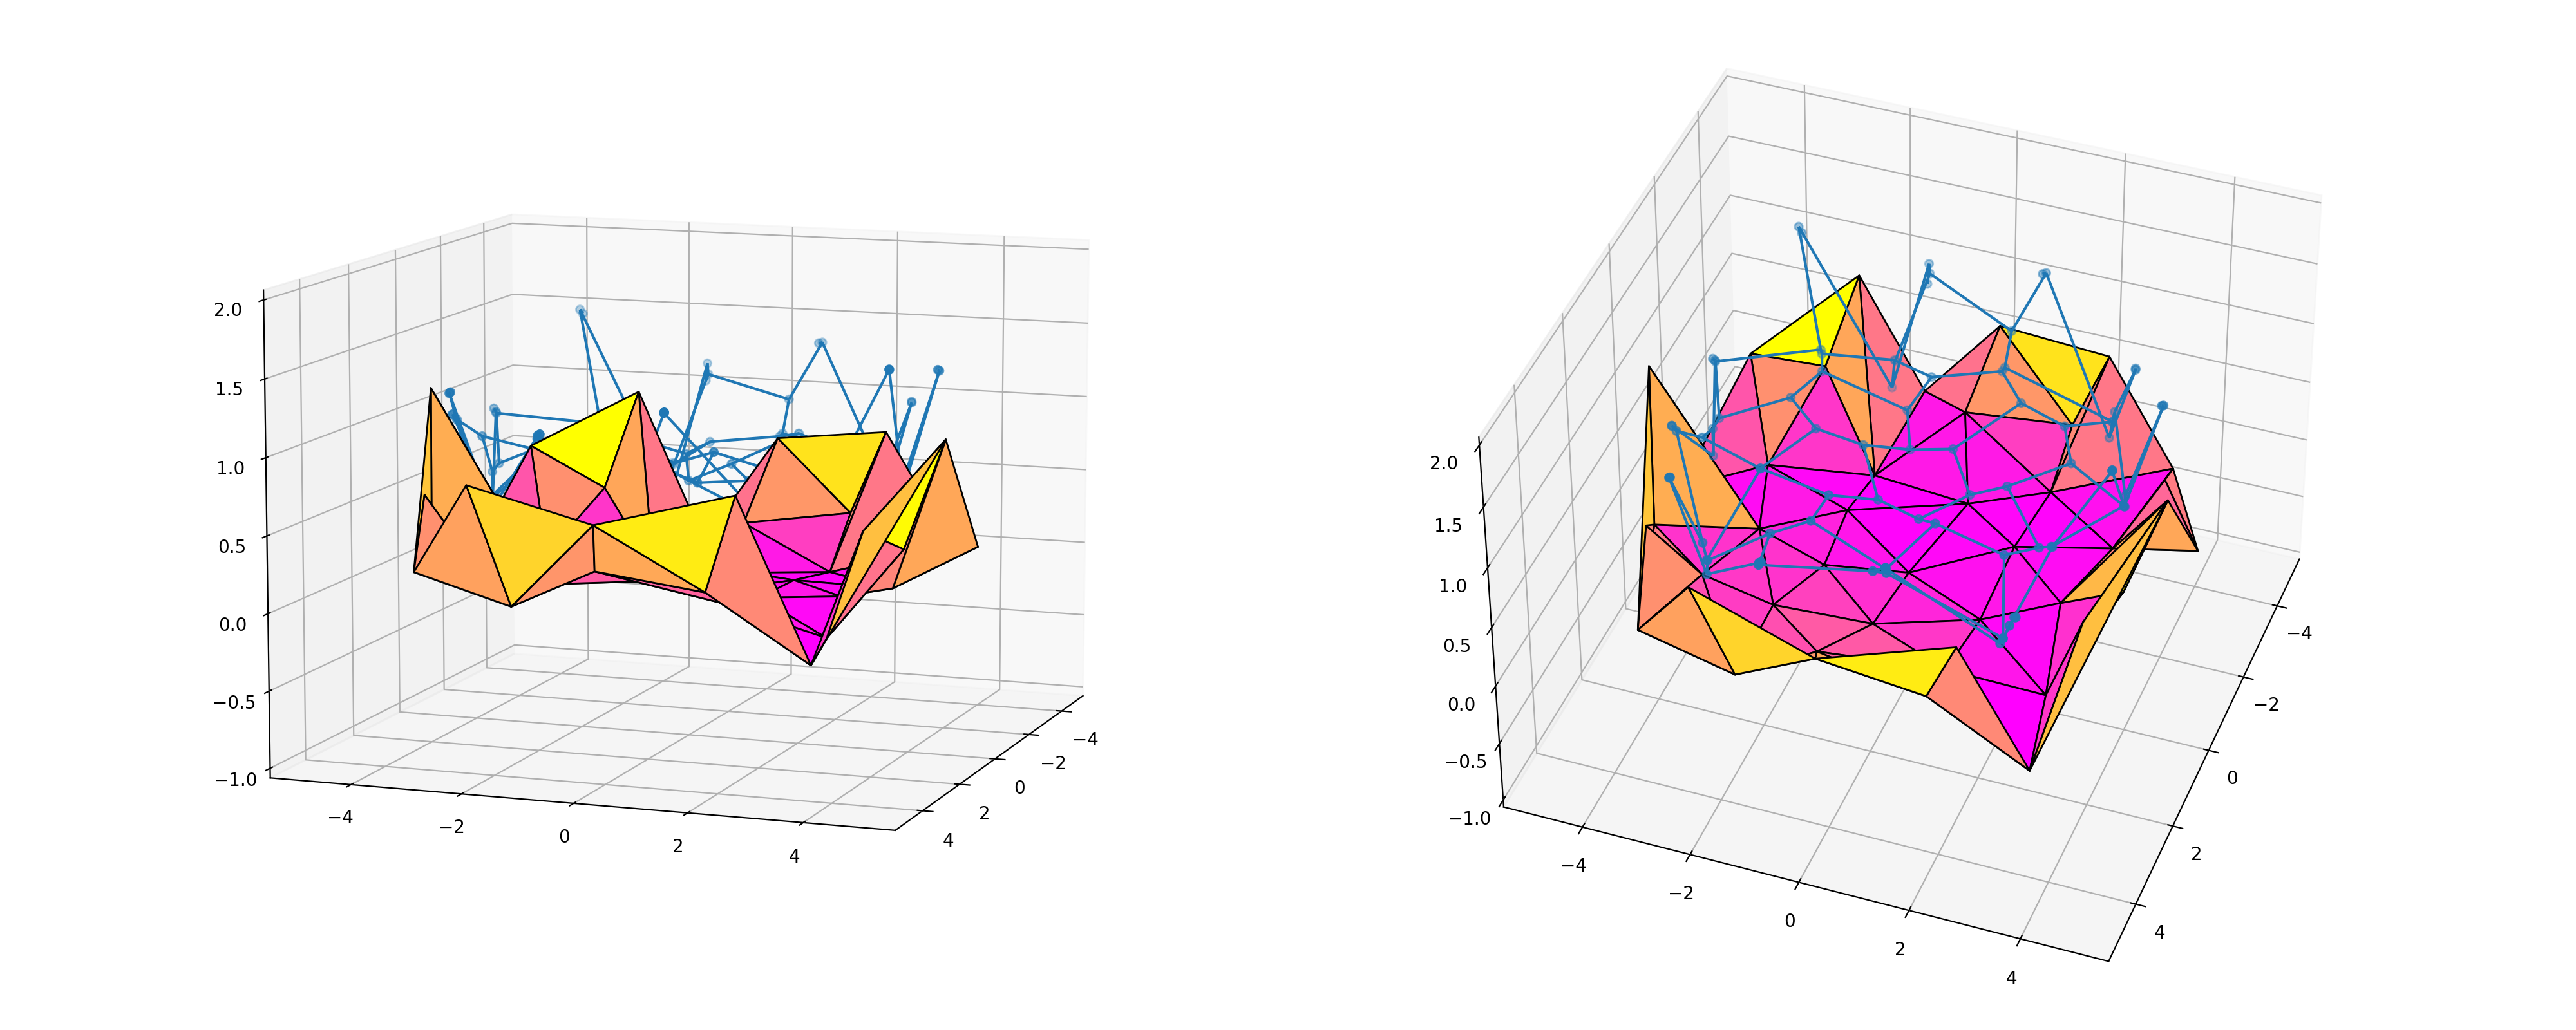
\includegraphics[width=0.69\textwidth]{hexbig/hexbig0.95_0.8_1.35_10_plot.png}
        \caption{Sheet shape when $\phi_0=0.95$, $\psi_0=0.8$, $\ell_0=1.52$.}
        \label{subfig:hexbig_out}
    \end{subfigure}
    \caption{Cell sheet geometry with a node of degree 7. The graph topology is affected in the sheet interior (subfigure \ref{subfig:hexbig_graph}). This minor change has substantial effects on the sheet geometry (subfigures \ref{subfig:hexbig_in}, \ref{subfig:hexbig_out}).}
    \label{fig:hexbig}
\end{figure}

